\documentclass[10pt, letterpaper]{article}
\usepackage[utf8]{inputenc}
\usepackage{graphicx}
\usepackage{subcaption}
\usepackage{lipsum}
\usepackage{wrapfig}
\usepackage{eso-pic}
\usepackage{soul}
\usepackage{xcolor}
\usepackage[parfill]{parskip}
\usepackage{tabularx}
\usepackage{longtable}
\usepackage{gfsdidot} % Use the GFS Didot font: http://www.tug.dk/FontCatalogue/gfsdidot/
\usepackage{microtype} % Improves typography
\usepackage[toc,page]{appendix} % creates an appendix
\usepackage{fancyhdr}
\usepackage{pdfpages}
% \usepackage{pagecounting}
% \usepackage[dvips]{color}

\newcommand{\illinoislogo}{
\includegraphics[height=0.5in]{images/illinoislogo.png}}
\newcommand{\anslogo}{\hspace{-4mm}
\includegraphics[height=0.5in]{images/ansuiuc.png}}
\newcommand{\anssite}{ans.npre.illinois.edu}
% \usepackage{background}
\usepackage{float}
\usepackage[top=2cm, bottom=2cm, outer=2cm, inner=2cm]{geometry}
\setcounter{tocdepth}{3}
% \setcounter{secnumdepth}{3}
\usepackage{environ}
\NewEnviron{letter}{%
  \input{structure}
  \opening
  \closing
}


\graphicspath{{./images/}}


% Creates the flow chart for conference management
\usepackage{varwidth}
\usepackage{tikz}
\usetikzlibrary{trees}
\usetikzlibrary{shapes.geometric, arrows}

\tikzstyle{chair} = [rectangle, rounded corners, minimum width=2cm, minimum height=1cm,text centered, draw=black,thick, fill=blue!50, execute at begin node={\begin{varwidth}{2.5cm}},execute at end node={\end{varwidth}}]
\tikzstyle{director} = [rectangle, rounded corners, minimum width=2cm, minimum height=1cm,text centered, draw=black, fill=orange!70, execute at begin node={\begin{varwidth}{2.5cm}},execute at end node={\end{varwidth}}]
\tikzstyle{coordinator} = [rectangle, rounded corners, minimum width=2cm, minimum height=1cm,text centered, draw=black, fill=white!30, execute at begin node={\begin{varwidth}{2.5cm}},execute at end node={\end{varwidth}}]
% \tikzstyle{arrow} = [thick,--,>=stealth]


\begin{document}
% ======================================================================================================
% DO NOT EDIT THIS SECTION
% ======================================================================================================
\begin{titlepage}
\AddToShipoutPictureBG*{\includegraphics[angle=90, width=\paperwidth,height=\paperheight]{earth1.png}};

   \begin{center}

       % \vspace{0.15cm}
 
       \Huge\color{white}\textbf{Saving the World One Atom at a Time}
 
       % \vspace{0.1cm}
       Nuclear, Plasma, and Radiological Engineering
 
       \vfill
       \vspace{8.5cm}
 
       
\includegraphics[width=0.4\textwidth]{ans_sc_logo3.png}

       \vspace{1cm}
 
       \Large\textbf{Presented by ANS at the University of Illinois Urbana-Champaign}
 

   \end{center}
\end{titlepage}
% ======================================================================================================
% ======================================================================================================
% ======================================================================================================

\clearpage
\newpage

\setlength{\headheight}{25pt}
\pagestyle{fancy}
\lhead{\anslogo}
\rhead{\illinoislogo}
% \renewcommand{\headrulewidth}{0pt} % no line in header area
% \fancyhead{}


\includepdf[pages=-]{./documents/chair_letter.pdf}

\newpage
\tableofcontents
\newpage

\section{Saving the World One Atom at a Time}
The future is nuclear. There are many grand challenges facing the world today and some have been designated existential threats to humanity. Young people today will witness the growing toll of anthropogenic climate change. As students, obstacles at the scale of the world climate crisis appear daunting and overwhelming. We believe that many solutions will come from the nuclear sciences. The ANS Student Conference is an opportunity for students and professionals to come together and share advances in critical technology and research dedicated to solving these problems. Nuclear, plasma, and radiological engineering will be central to many endeavors, whether the goal is solving the world’s energy needs, developing technology that will take us to the stars, or curing cancer. By hosting this conference, we hope to inspire and motivate students in these engineering fields to tackle big problems. Saving the World One Atom at a Time reflects the fact that nuclear science is a powerful force in dealing with grand challenge problems. This theme also honors the individual, atomic, contributions from students, researchers, and professionals that are essential to progress. This conference is about science and engineering and it is about the people that make science and engineering possible. Students will hear from visionary speakers and leaders of the nuclear science community and come away with optimism for the future; knowing that they are saving the world one atom at a time.\\
There are three main goals of our theme and each of these goals will be the focus of a different day of the student conference.
\begin{enumerate}
	\item Celebrate the people behind the science and engineering.\\
	Everyone that does science has a unique background, skillset, and experiences. People are what make science possible. Encouraging diversity and inclusivity in these areas, and others, improve creativity, productivity, and insights. We showcase this aspect of the conference with panels like \textit{Science is People: How to Conduct Inclusive Research} and \textit{Scientific Storytelling}.
	\item Connect students and professionals to develop strong networks.\\
	This is the networking and professional-development-focused section of the conference. Beyond the mere job-seeking aspect, these networks enable the spread of ideas. Additionally, this evening builds on top of the previous night as we remember that our networks also consist of people. More diverse networks are better networks. This aspect of the conference is captured by workshops like \textit{Developing Your Network}. 
	\item Inspire the next generation of nuclear engineers to take on grand challenge problems.\\
	The final day is the culmination of the conference and underpins the single unifying ideal. For many students, this conference might be the first time they are presenting research to their peers, mentors, and future employers. Everything about this conference should encourage students to take on challenges that seem bigger than they are in order to improve the world around them.  
\end{enumerate}
These goals and our theme motivated every decision in our conference proposal. The University of Illinois at Urbana-Champaign chapter of ANS would be honored to host the 2021 student conference. We hope to create an atmosphere that will galvanize students and professionals for the exciting future of nuclear engineering.\\

\newpage
\section{Welcome to Illinois}

\begin{figure}[H]
  \centering
  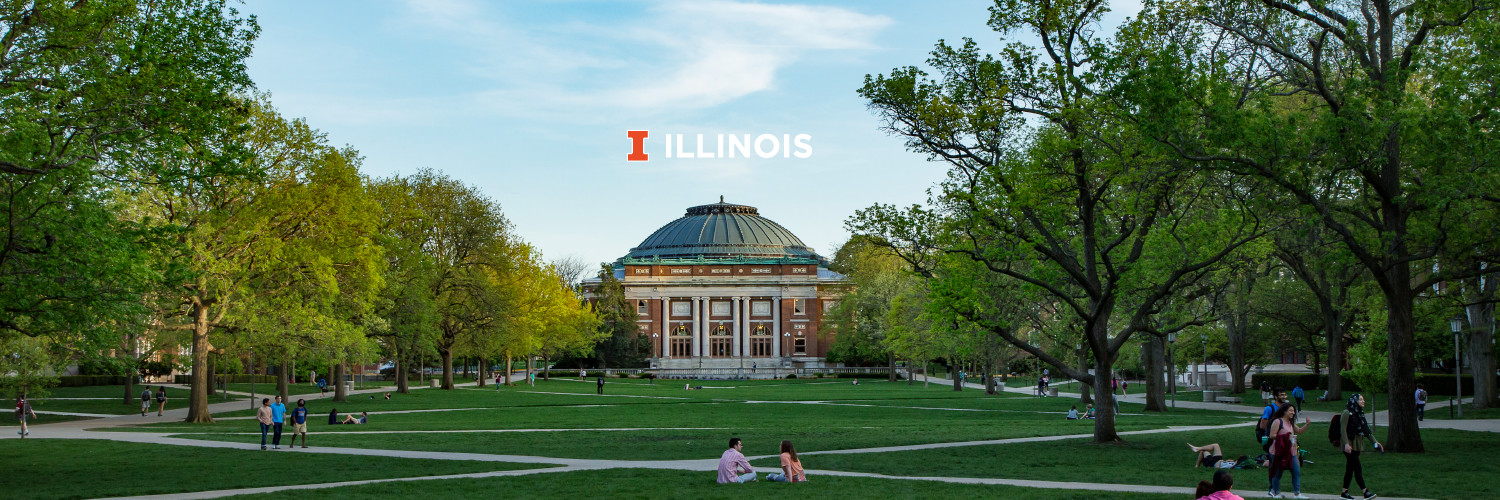
\includegraphics[width=\textwidth]{illinois-main.jpeg}
\end{figure}

\subsection{Champaign-Urbana in a Nutshell}
Champaign-Urbana (CU), colloquially known as Chambana, is home to the state's flagship school, the University of Illinois at Urbana-Champaign (UIUC). Since its founding in the mid 19th century CU has grown into the flourishing cultural hub of the midwest it is today. CU houses many landmarks and districts, and showcases both local and national events annually. It is home to the Historic Virginia Theater that hosts Ebertfest in honor of the late film critic and UIUC alumnus Roger Ebert. The Krannert Center for the Performing Arts is located on U of I campus, which is known for its four first-class venues, including the Foellinger Great Hall - one of the most acoustically perfect performance spaces in the world, attracting world famous artists and ensembles to perform there every year. Other notable events that attract many people to the twin cities are the Pygmalion Music Festival, the Urbana Sweetcorn Festival, and the Illini Marathon. 

\begin{wrapfigure}{r}{0.35\textwidth}
  \begin{center}
  \vspace{-\baselineskip}
    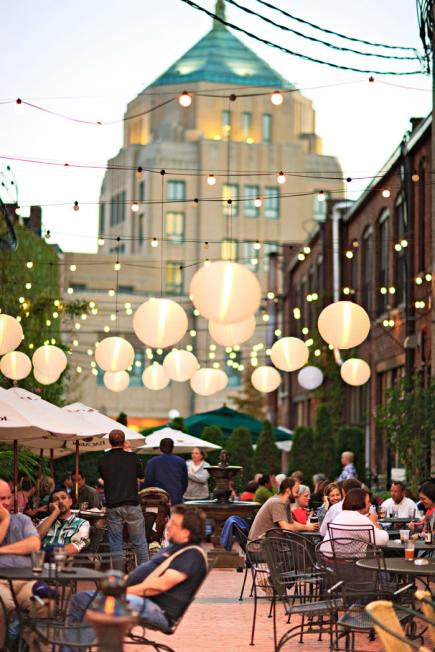
\includegraphics[width=0.33\textwidth]{chm1.png}
    \caption{Downtown Champaign}
  \end{center}
\end{wrapfigure}


CU is an industrial base to several major companies including Abbott Laboratories, Archer Daniels Midland (ADM), Caterpillar, John Deere, The Dow Chemical Company (TDCC), IBM, and State Farm. Other top employers in CU include Kraft Heinz, Carle Foundation Hospital, and Wolfram Research. Carle has notably been affiliated with the creation of the first college in CU in over 60 years, the Carle Illinois College of Medicine -  ``the world's first engineering-based college of medicine". Research Park at the University of Illinois serves as a technology hub for several research and development ventures, where there are more than 120 companies employing 2,100 students and professionals in high-technology careers.

The state of Illinois relies heavily on nuclear power to supply its energy needs with 52$\%$ of electricity generated by nuclear plants. The first human controlled nuclear reaction, Chicago Pile One, happened in Illinois. UIUC also bears a long tradition of nuclear power research and was home to the TRIGA nuclear reactor for almost 40 years. During this time researchers at UIUC contributed to the knowledge store of nuclear reactor kinetics, isotope production, fission fragment physics, and much more. Now, UIUC is exploring ways to use nuclear power to accelerate its decarbonization efforts. This exploratory effort has the potential to position UIUC as the world leader in advanced carbon-free technologies. We hope to continue our excellent nuclear tradition by hosting the ANS Student Conference in 2021. 
\clearpage

\subsubsection{Accessibility and Accomodation}
 A large number of hotels are located around downtown Champaign and the Eastern side of campus, making transportation easy. Champaign-Urbana Mass Transit (CU-MTD) is a reliable public transportation service that sees millions of riders every year. CU-MTD charges an affordable rate of \$1 per ride, which can be paid in cash or using the Token Transit app. Additionally, an all-day pass can be bought on Saturdays and Sundays for \$2 from any bus operator or from the app. All CU-MTD busses are wheelchair accessible. Rental bikes and rideshare services are also plentiful. There is a small airport, Willard Airport, just 20 minutes from campus that has regular flights to and from Chicago O’Hare and Dallas Fort Worth airports. Finally, Peoria Charter is a popular bus service with several daily trips between the UIUC campus and the Chicagoland area.

\subsubsection{Weather}
With an average high temperature of 65$^{\circ}$ and an average low temperature of 40$^{\circ}$, April in Champaign is a gorgeous month of dwindling winter weather and spring coming into bloom. Holding a conference during this time would be the perfect way to showcase our beautiful city.

\subsection{University of Illinois at Urbana-Champaign: Learning \& Labor}
\begin{wrapfigure}{r}{0.5\textwidth}
  \begin{center}
  \vspace{-\baselineskip}
    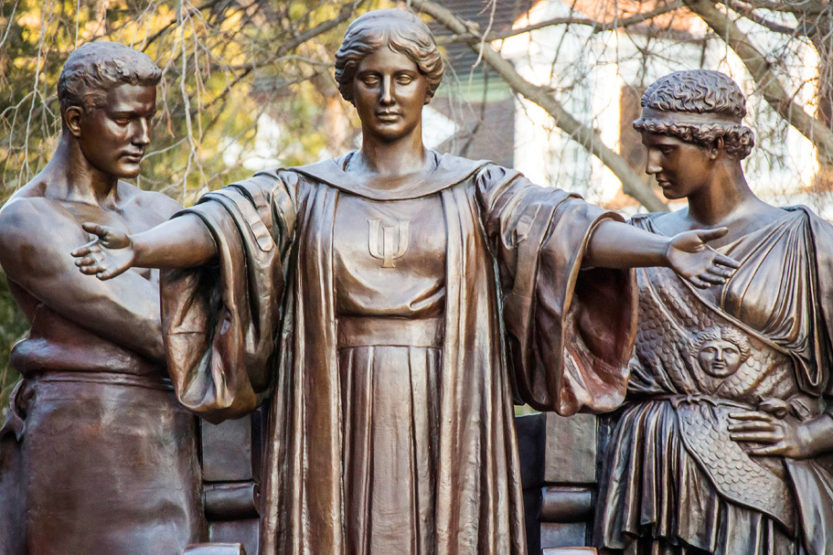
\includegraphics[width=0.44\textwidth]{alma.jpg}
    \caption{Alma Mater accompanied by Learning and Labor}
  \end{center}
\end{wrapfigure}
Founded in 1867, the University of Illinois at Urbana-Champaign (UIUC) has cultivated a long history of significant scientific discoveries and contributions. The theory of superconductivity, the invention of the transistor, the discovery of archaea, the fourth domain of life, and the first web browser are just some of the many breakthroughs that came out of UIUC. The famous Morrow Plots, established in 1876, became the first research crop field at a university and is still used today. Attendees might also be familiar with Blue Waters, one of the world’s fastest supercomputers. 
The UIUC Grainger College of Engineering has had sixteen Nobel Laureates in physics. Including John Bardeen, the only scientist to ever win the award in physics twice. It also offers 15 different majors to almost 6000 undergraduate and 2500 graduate students. Of its twelve ranked majors, nine are ranked among the top 10 in the nation, and six of which remain ranked among the top 5 in their degree. Overall, the Grainger College of Engineering in Urbana-Champaign ranks sixth among the nation’s best undergraduate engineering programs. With more than 250 degrees for undergraduates and graduates and a multitude of first-class research facilities and resource, UIUC gives its nearly 45,000 students the ability to succeed. 

\subsection{UIUC ANS Student Chapter (ANS-UIUC)}

The ANS-UIUC maintains and develops a cohesive community of students in nuclear engineering. It also engages in education and outreach programs to teach members of the surrounding community about nuclear science. One of our most popular outreach programs is Engineering Open House (EOH), during which ANS-UIUC repeatedly earns awards for best presentation of a society. EOH is an annual event where members of the local community, from young children to senior adults, visit the engineering campus to learn more about STEM research. Membership is currently around 70-80 students and has been steadily growing. The chapter works to host events catering to nuclear, plasma, and radiological concentrations. Professional development plays a crucial role in student development, and it is the biggest part of member involvement at UIUC. Professional development activities range from tours of various facilities to pizza with campus visitors. Some of the past tours have included Clinton Power Station, Curium Pharma through UIUC Women In Nuclear, Oak Ridge National Laboratory, Analysis System (ANSYS) Inc, and Argonne National Laboratory. ANS-UIUC has historically been one of the best represented institutions at the annual student conference and is a tradition this chapter is eager to uphold. 

\begin{figure}[H]
  \centering
  \includegraphics[scale=0.15]{eoh1.JPG}
  \caption{Mouse Trap Chain Reaction at EOH 2019}
\end{figure}

\begin{figure}[H]
  \centering
  \begin{subfigure}{0.5\textwidth}
    \centering
    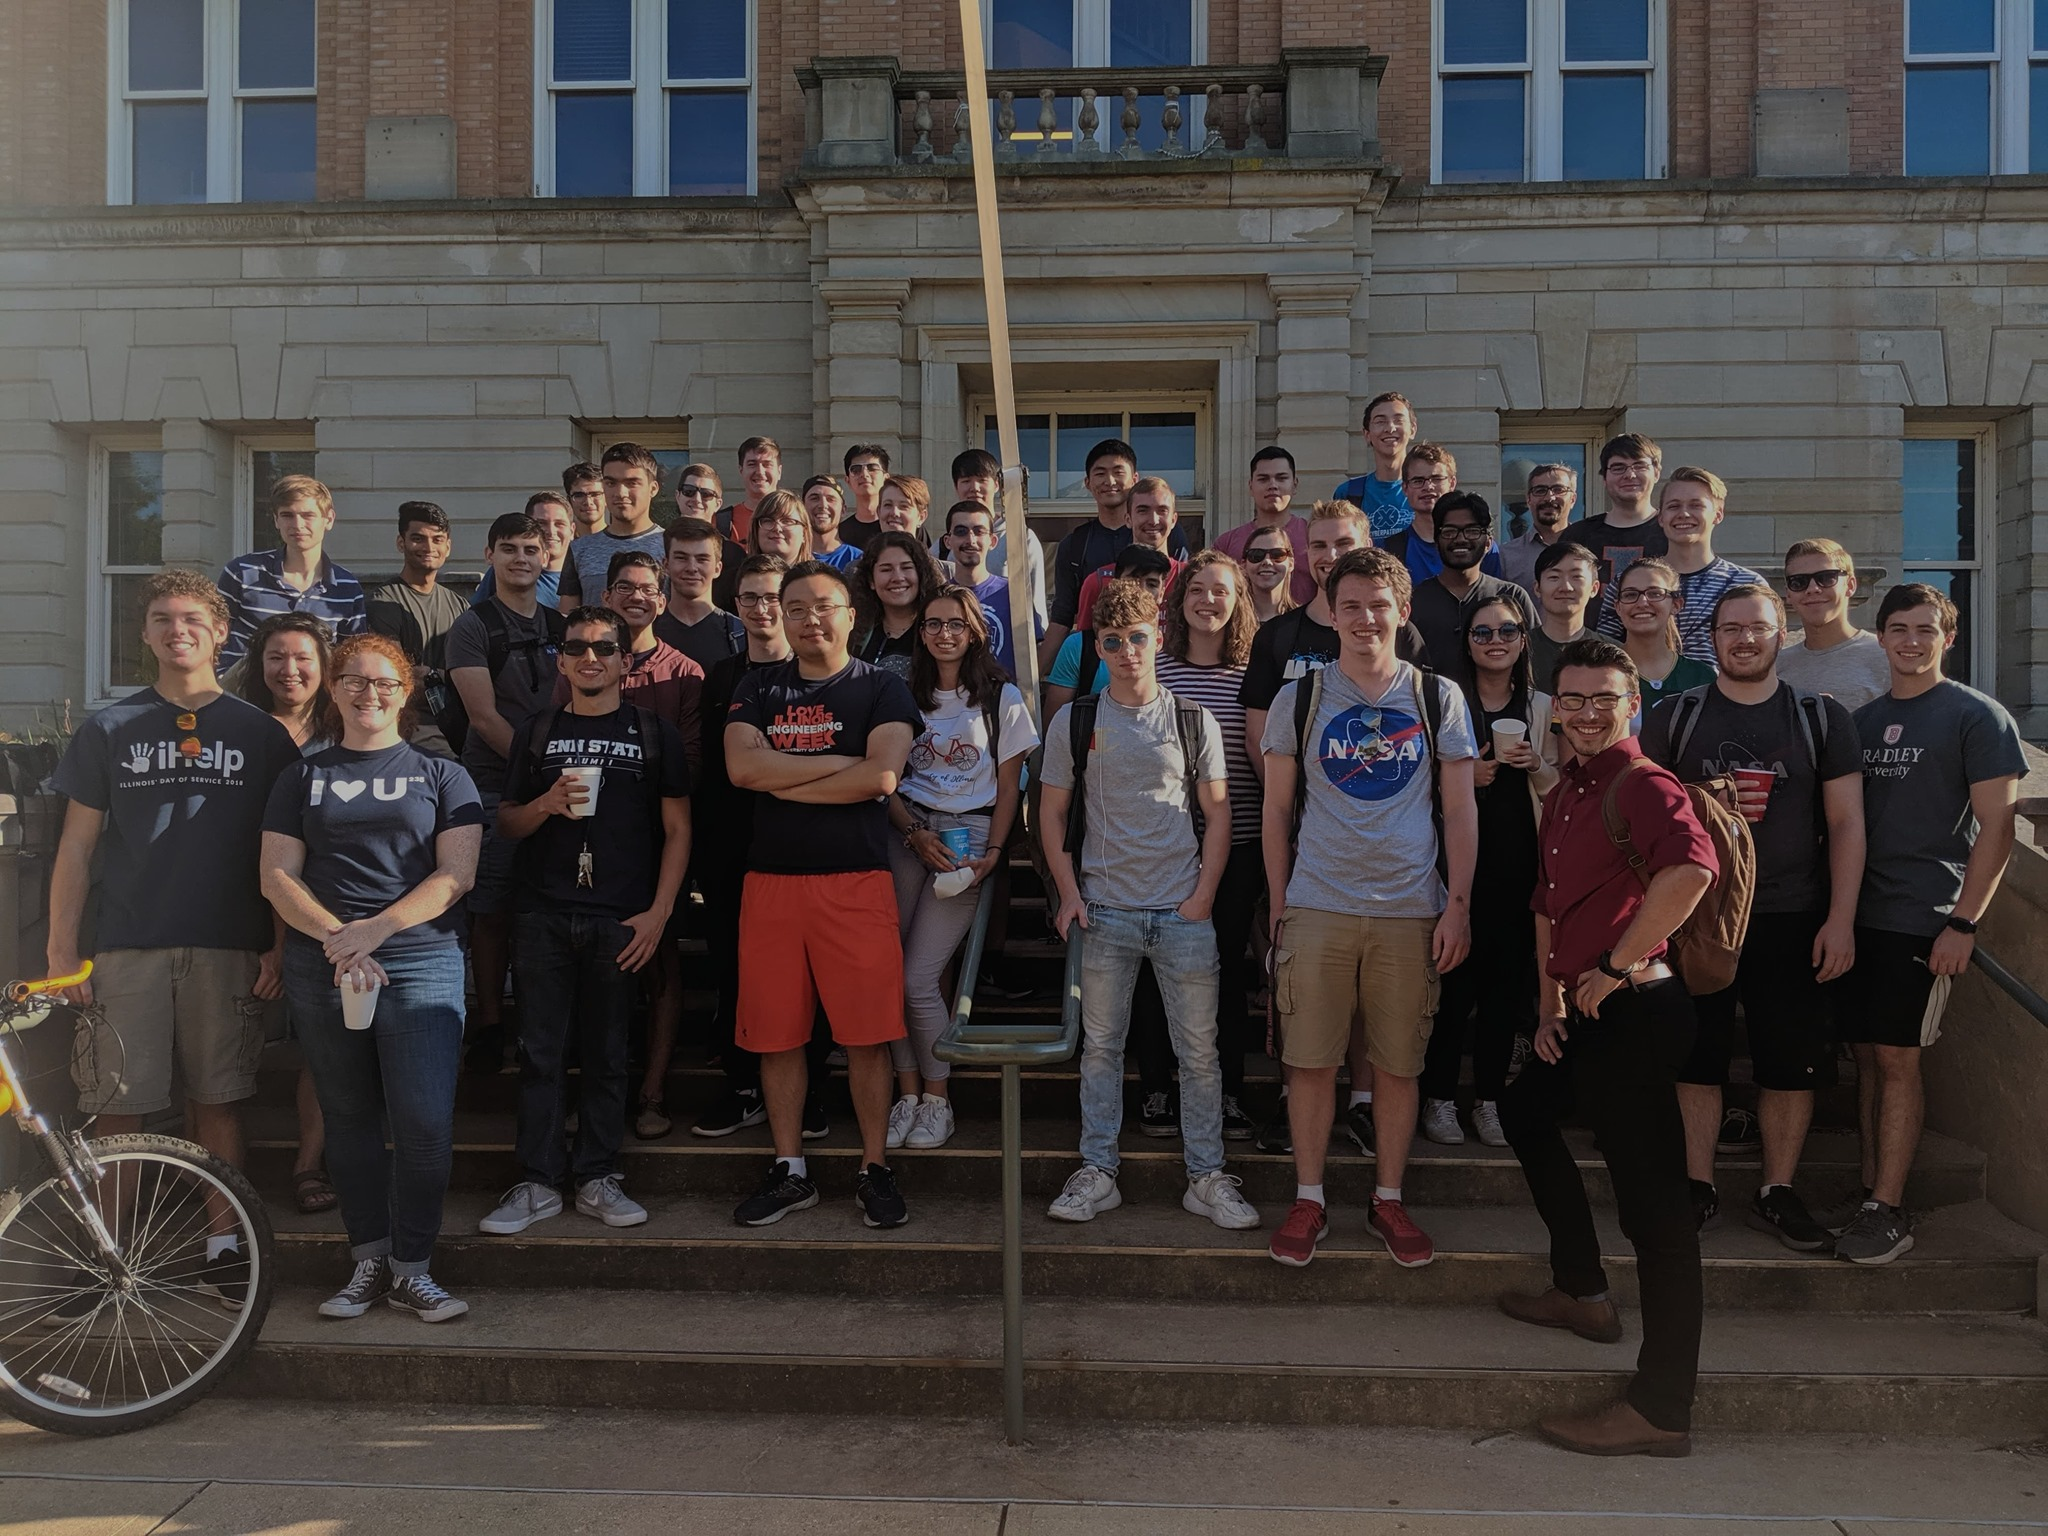
\includegraphics[width=8cm]{ans_uiuc_group.jpg}
    \subcaption{ANS Barbeque 2019}
  \end{subfigure}%
  \begin{subfigure}{0.5\textwidth}
    \centering
    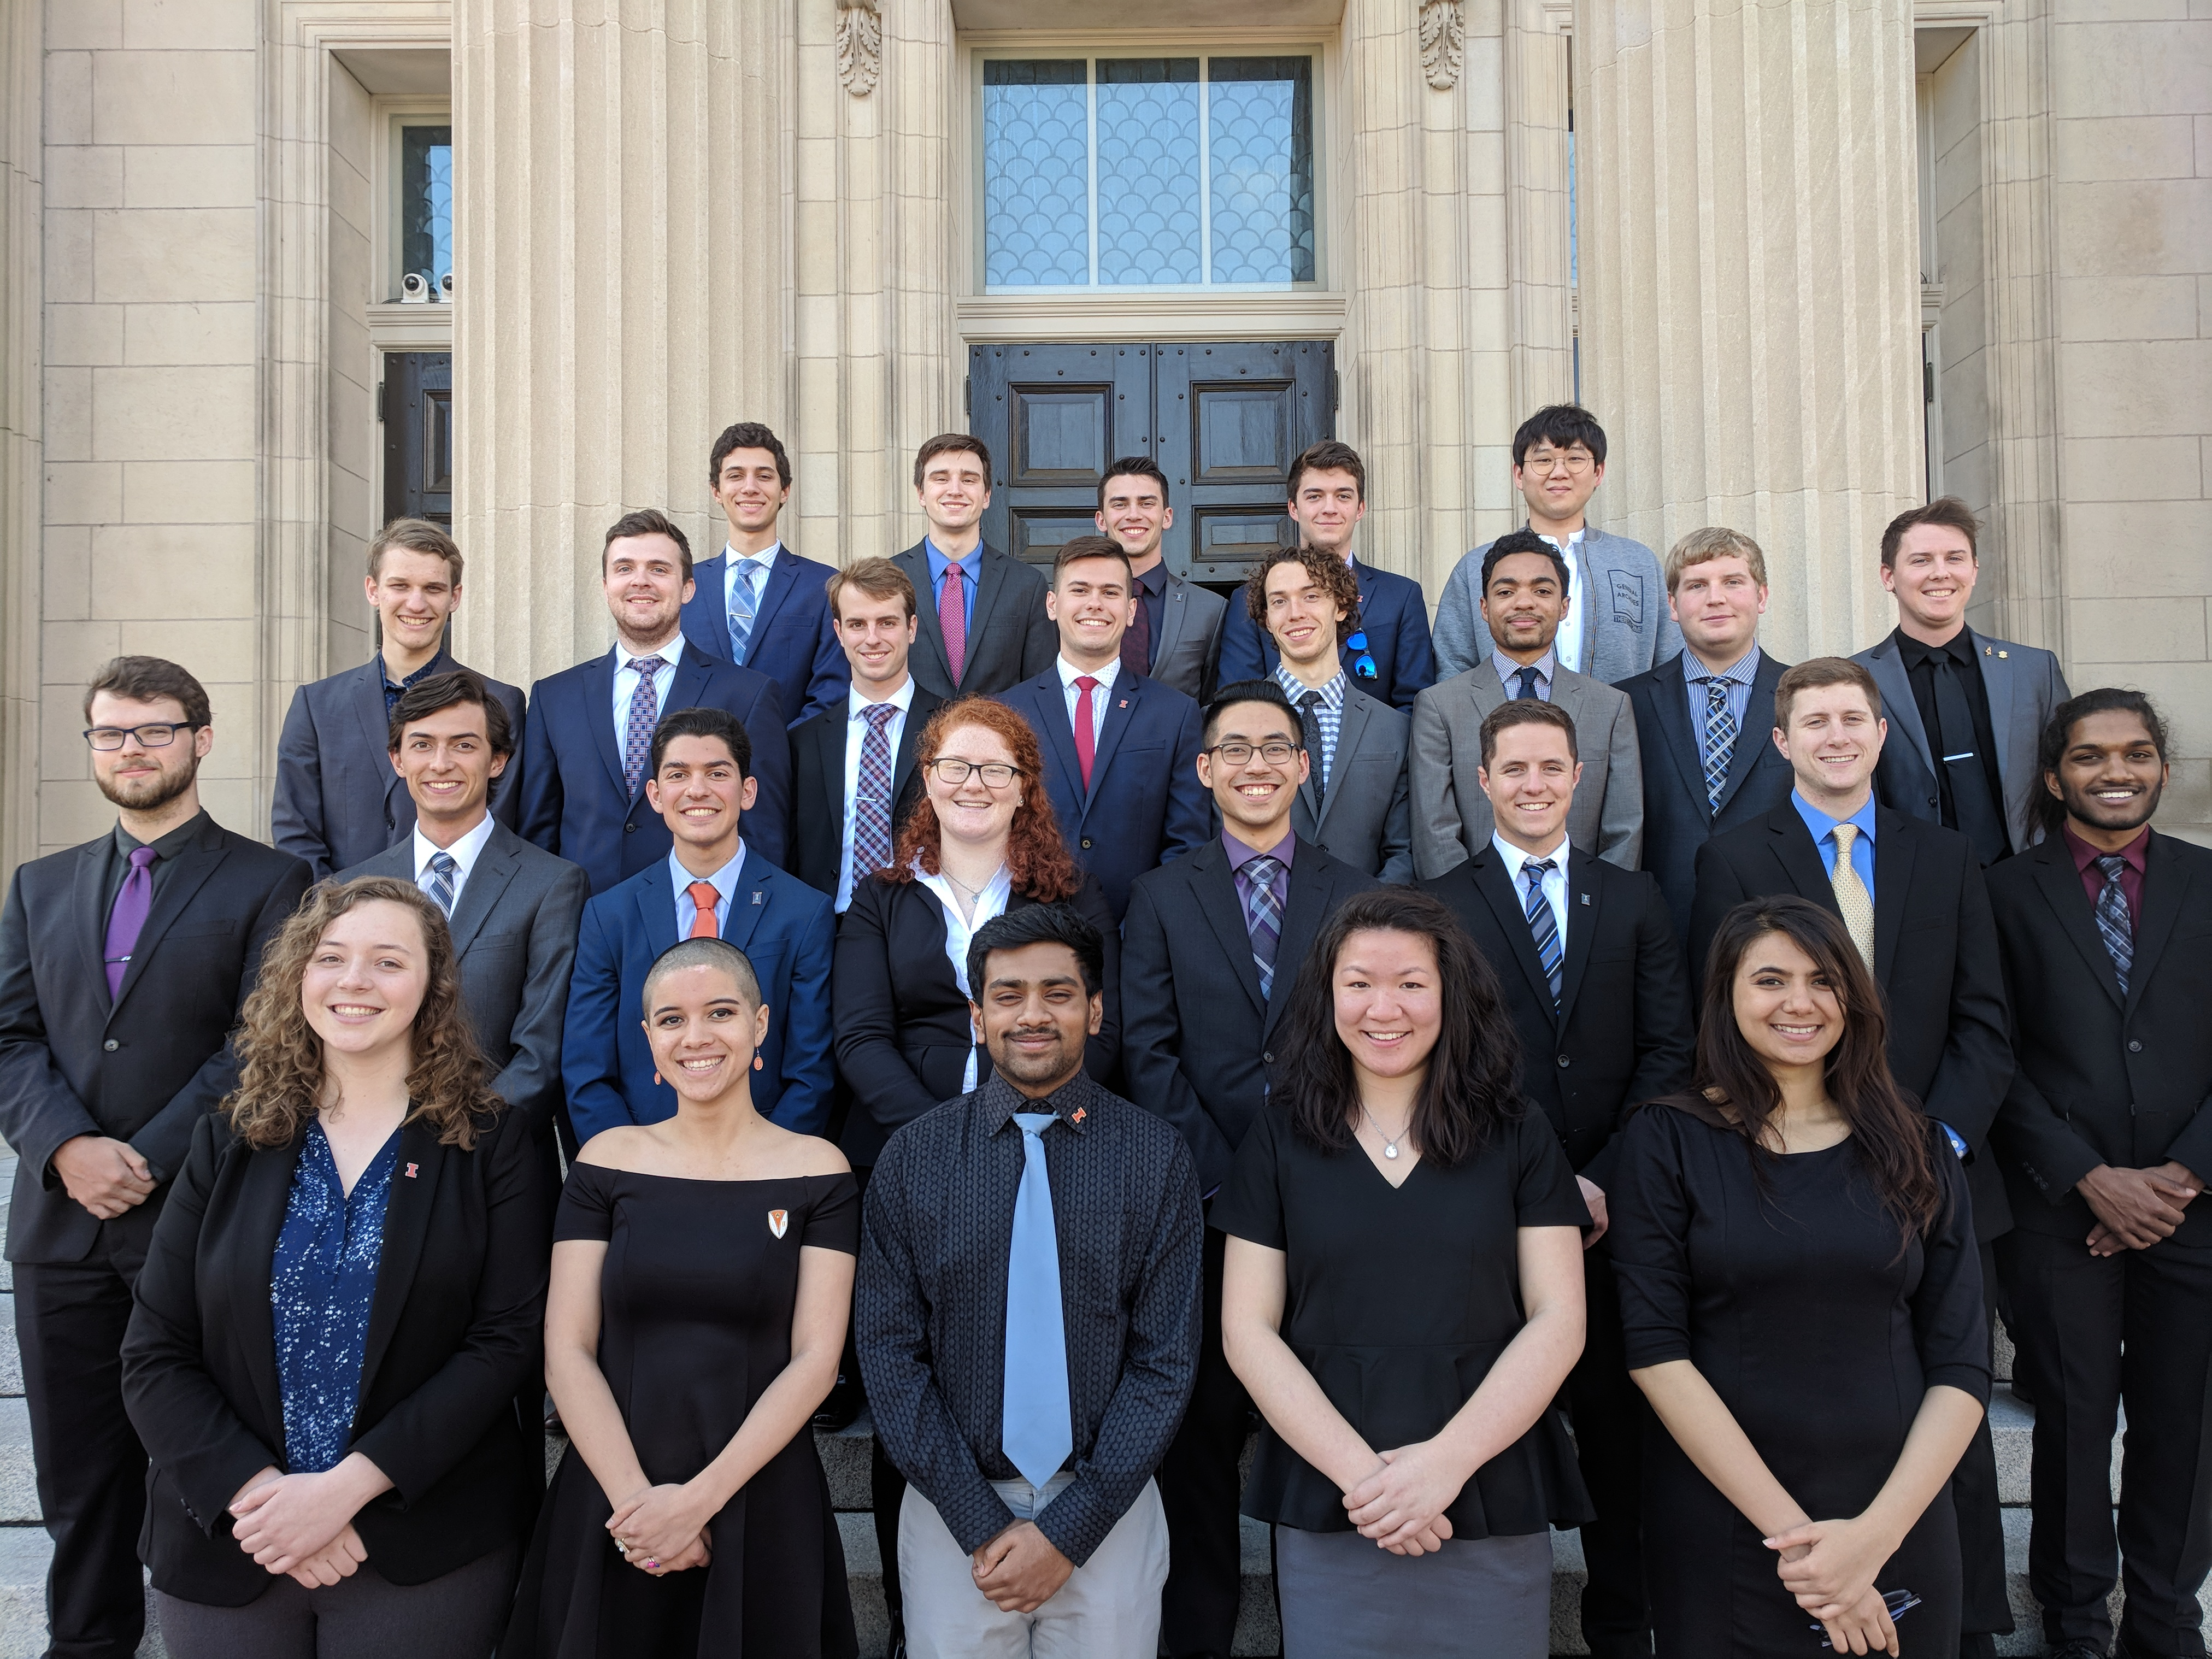
\includegraphics[width=8cm]{ans_conf_19.jpg}
    \subcaption{ANS Student Conference 2019 at VCU}
  \end{subfigure}   
\end{figure} 

\clearpage

\subsection{Research at UIUC}
Faculty and students in the Department of Nuclear, Plasma, and Radiological Engineering (NPRE) at Illinois conduct research in many areas of interest to the nuclear science community. Both graduate and undergraduate  students actively participate and make their own atomic contributions that will someday save the world.
Research programs in Nuclear, Plasma, and Radiological Engineering at the University of Illinois at Urbana-Champaign can be
broadly classified into five areas:
\begin{itemize}
        \item \textbf{Nuclear Power} (reactor physics, thermalhydraulics, fuel cycle, radiation transport, I\&C)
        \item \textbf{Plasma and Fusion} (modeling, plasma-material interactions)
        \item \textbf{Radiological Sciences} (detectors, imaging, health physics, medical applications)
        \item \textbf{Material Science} (nuclear fuels, structural materials)
        \item \textbf{Risk and Policy} (PRA, safety, energy, arms controls, disarmament, security)
\end{itemize}

These research areas are supported by a stellar faculty and world-class facilities, which 
will be briefly described below.

\subsubsection{Nuclear Power}
NPRE is well known for its pioneering research in the area of reactor power engineering. Graduates have gone on to leadership positions in industry, national laboratories, and academia. Research in the Nuclear Power concentration covers all aspects of power generation using nuclear energy on land, underwater (submarine), and in space. It is inherently interdisciplinary and relies on several branches of physics and engineering for design and analysis of large complex systems. These include aspects of reactor physics, reactor thermal-hydraulics, reactor safety, reliability and risk, instrumentation and control, training and education, human factors engineering, reactor materials, nonproliferation, and more. Safety standards and maintenance for existing reactors and new reactor designs are also explored by faculty in the department. Crosscutting areas of research include multi-physics and multi-scale modeling and simulation, high performance computing, reliability and risk, validation and verification, and uncertainty analysis. Recently, the University of Illinois declared a plan to be completely carbon-neutral by 2050. Nuclear power is the perfect candidate to help UIUC attain its carbon reduction and energy goals. Together, the University and the NPRE department are saving the world one atom at at time.

\subsubsection{Plasma Physics and Fusion Science}
\begin{wrapfigure}{r}{0.5\textwidth}
  \begin{center}
  \vspace{-\baselineskip}
    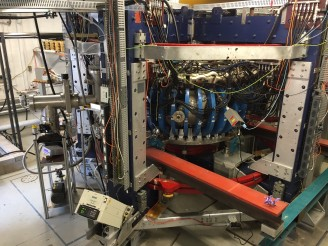
\includegraphics[width=0.48\textwidth]{hidra.png}
    \caption{The Hybrid Illinois Device for Research and Application (HIDRA)}
  \end{center}
\end{wrapfigure}
The Fusion and Plasma Physics research theme in the NPRE department has a long history of work in the area of magnetic and inertial nuclear fusion as well as plasma engineering. NPRE is now one of the leading departments in plasma-material interactions with its Center for Plasma-Materials Interactions established by Prof. David Ruzic. Furthermore, in the past few years, two new faculty members have been added to this area including: Prof. Davide Curelli and Prof. Daniel Andruzcyk. There are five research themes that spans the work in fusion and plasma physics: fusion materials, plasma-material interface (PMI) diagnostics, plasma-edge and PMI modeling, plasma nanosynthesis, and plasma sources and processing. The Hybrid Illinois Device for Research and Application (HIDRA) marks the newest addition to the team at CPMI. This device finished construction and achieved first plasma during the spring of 2016. \\

\subsubsection{Radiological Science}
Radiological engineering at UIUC strives to discover novel applications for ionizing radiation in biomedical research, homeland security, and nuclear safeguards. We have developed various gamma-ray, x-ray and neutron detectors, imaging devices, and novel algorithms for analyzing the data from these systems. These algorithms range from the use of so-called "big data" techniques applied to large sensor networks to advanced radiological imaging methods and image processing techniques for biomedical research. We work with physicists, biologists, chemists, material scientists, statisticians, and physicians around the world, to develop advanced diagnostic imaging and radiation-induced therapeutic approaches to address some of the most critical health care-related issues, such as cancer, cardiac diseases, diabetes and neurodegenerative disorders. We also work with organizations like the Departments of Defense, Energy, and Homeland Security and the International Atomic Energy Agency to deploy our research around the world to detect and identify the illicit movement of nuclear and radiological materials.

\subsubsection{Reliability and Risk Analysis}
Risk analysis represents the pinnacle of interdisciplinary research and education. Following the Three Mile Island disaster in 1979, Probabilistic Risk Assessment (PRA) has become a key pillar of the risk-informed nuclear regulatory framework, and is now a requirement for every nuclear power plant in the United States. Enhancing the prevention of catastrophic technological accidents and the protection of the environment requires advancement in multidisciplinary PRA. It demands the development of a common vocabulary within diverse engineering and social science domains in order to address risks that emerge from the interface of social and technical systems.


\subsubsection{Materials Science}
Materials science research includes investigations of the mechanical properties of cladding and other structural components, and heat exchanger materials. Advanced microanalysis techniques are often employed to perform nano-scale interrogation of deformation, precipitation, and chemical segregation studies, etc. Ion beam bombardment of materials is often used with these techniques to simulate fast neutron displacement cascade damage. Fuel performance modeling, molecular dynamics, and kinetic Monte Carlo simulations complement these experimental activities. The department also has strong efforts related to the study of nuclear fuel such as urania, including mass transport and mechanical property studies. The department also studies hydrogen in metals, including hydride phase formation and solute dislocation pipe diffusion.

\subsubsection{NPRE Research Groups and Laboratories}
The faculty, pictured in Figure \ref{fig:faculty} support the above areas of 
expertise in the collaborations and facilites discussed below.

\begin{figure}[htbp]
        \begin{center}
                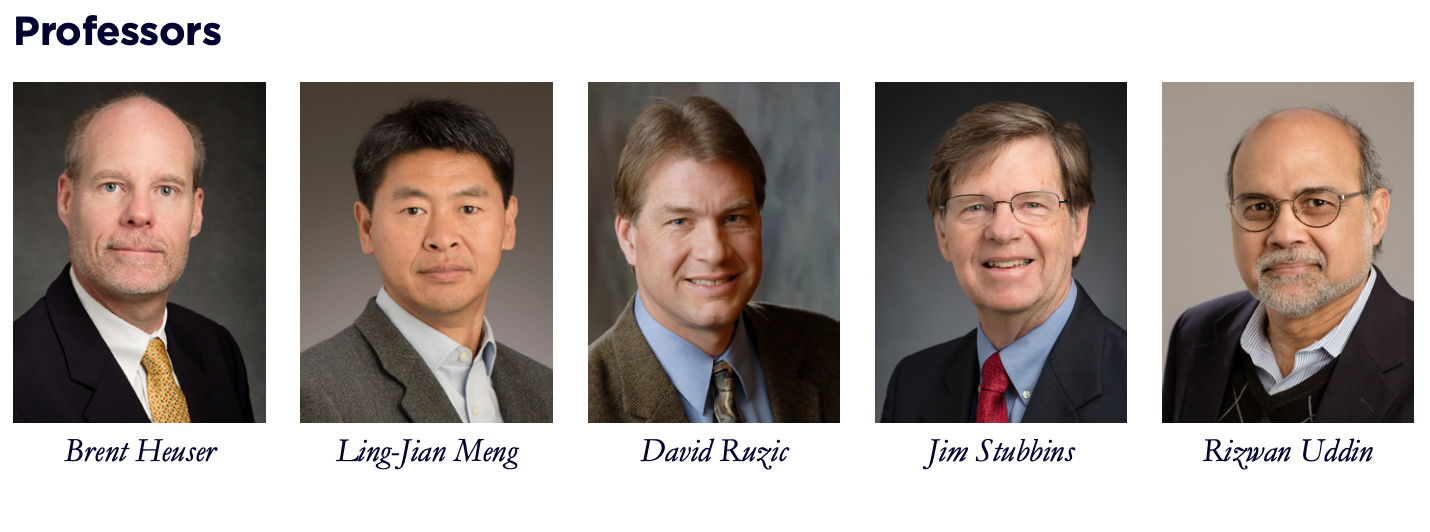
\includegraphics[width=0.75\textwidth]{./images/full.png}
                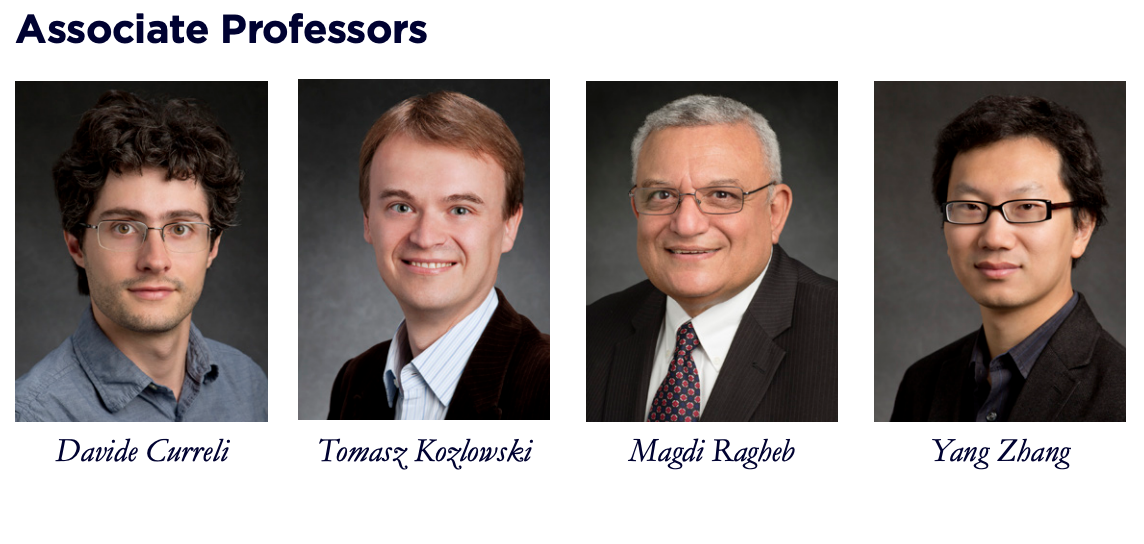
\includegraphics[width=0.6\textwidth]{./images/associate.png}
                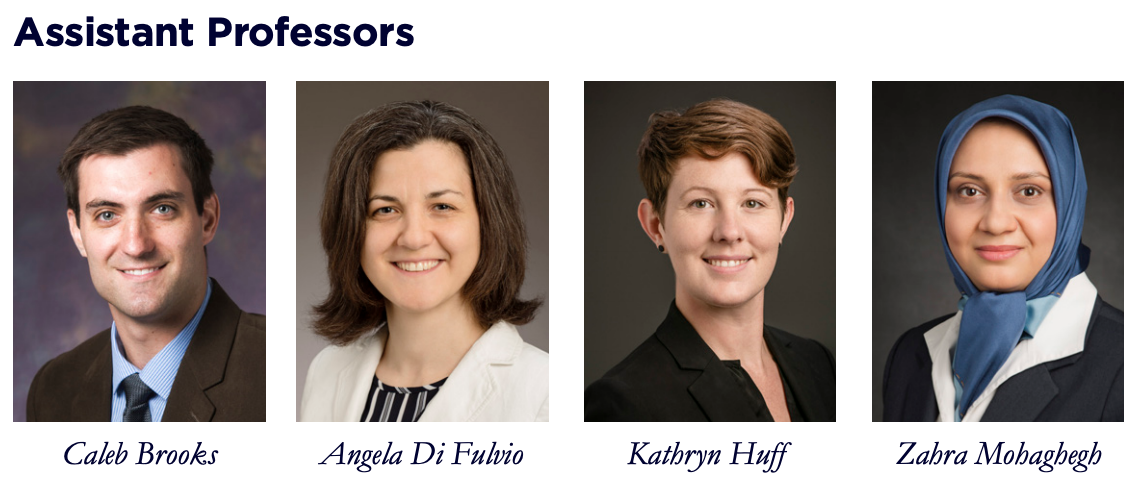
\includegraphics[width=0.6\textwidth]{./images/assistant.png}
                
\includegraphics[width=0.3\textwidth]{./images/research.png}
        \end{center}
        \caption{Faculty in Nuclear, Plasma, and Radiological Engineering  at 
        the University of Illinois at Urbana-Champaign.}
        \label{fig:faculty}
\end{figure}

\begin{itemize}
  \item \textbf{Advanced Reactors and Fuel Cycles (ARFC)} - \textit{Dr. Kathryn Huff}\\
  The ARFC group seeks to advance the safety and sustainability of nuclear energy production through improved reactor designs, fuel cycle strategies, and waste management techniques. In the area of advanced reactors, our work focuses on extending current simulation tools with features essential to advanced reactor multiphysics. In the context of the broader nuclear fuel cycle, the ARFC group emphasizes modeling, simulation, and analysis of the global nuclear fuel cycle, with an emphasis on sustainability. A crosscutting theme of our research is an emphasis on advancing methods and software for computational nuclear engineering. Accordingly, the Advanced Reactors and Fuel Cycles group is proud to be affiliated with the University of Illinois National Center for Supercomputing Applications and its Blue Waters computing facility.
  \item \textbf{Virtual Education and Research Laboratory (VERL)} - \textit{Dr. Rizwan Uddin}\\
  The VERL group focuses on the development of innovative numerical methods and their implementation on high performance computing machines. Research efforts center on problems in nuclear engineering, with emphasis on thermal-hydraulics and reactor physics.

  \item \textbf{Analysis of Reactor Transients and Stability (ARTS)} - \textit{Dr. Tomasz Kozlowski}\\
  The ARTS group performs deterministic safety analysis by developing and validating advanced methods to accurately determine reactor safety margins and reactor behavior. By performing high-fidelity numerical predictions of the reactor behavior in abnormal transient scenarios of safety significance, our work supports the nuclear reactor safety analysis, and increases the fidelity of primary system simulation. This approach is at the heart of nuclear power’s excellent safety record – always striving to improve current tools and methods.

  \item \textbf{Center for Plasma-Material Interactions (CPMI)} - \textit{Dr. David Ruzic}\\
  The primary objective of CPMI is the study of plasma-material interactions relevant to fusion, semiconductor manufacturing, and plasma processing through a combination of experimental and computational means. CPMI has facilities for the study of fusion materials, High Power Impulse Magnetron Sputtering (HiPIMS), liquid metals, Extreme Ultraviolet Lithography (EUVL),  laser-material interactions, and more. Projects are supported by both government and commercial partners to further the application and knowledge of plasma physics. The facility recently finished the construction of the HIDRA fusion device, which is a stellarator-tokamak machine hybrid machine used to study plasma-materials interactions.  HIDRA is currently run by Dr. Daniel Andruczyk.

  \item \textbf{Materials Science} - \textit{Dr. James F. Stubbins}\\
  The group investigates a wide variety of topics within the realm of materials research including mechanical properties, microstructural evaluations, plus radiation damage investigations, and modeling. Materials such as copper alloys nickel-based alloys, stainless steels, ferritic steels, and silicon-carbide composites are studied using a variety of analytical techniques electron microscopy and spectroscopy.


  \item \textbf{Non-Equilibrium Matter Laboratory} - \textit{Dr. Yang Zhang}\\
  This laboratory focuses on the study of non-equilibrium matter, with particular emphasis on liquids and soft matter, using integrated neutron and synchrotron light experimental probes and atomistic modeling and simulation. The structure and dynamics of these systems are either inherently complex or driven away from equilibrium by extreme conditions. In particular, our current interests include a range of fundamental and technical problems involving slow phenomena and rare events, such as: materials far from equilibrium and in extreme environments; extreme properties of liquids; and glassy or jammed soft matters.

  \item \textbf{Radiation Imaging Group} - \textit{Dr. Ling Jian Meng}\\
  Research is on developing radiation sensor and systems for visualizing the distribution of radioactivity in surrounding objects, patients, and small lab animals etc. Current emphasis includes (a) developing novel radiation sensors for detecting X-ray, gamma rays and neutrons, and (b) developing nuclear techniques for detecting and imaging a tiny amount radiolabeled molecules inside small lab animals.

  \item \textbf{Socio-Technical Risk Analysis (SoTeRiA)} - \textit{Dr. Zahra Mohaghegh}\\
  The Socio-Technical Risk Analysis (SoTeRiA) Laboratory is evolving Probabilistic Risk Assessment (PRA) by explicitly incorporating the underlying science of accident causation into risk scenarios. SoTeRiA laboratory has pioneered two key areas of theoretical and methodological innovations: (1) spatio-temporal causal modeling of social and physical failure mechanisms in PRA, and (2) the fusion of big data analytics with PRA. The Lab’s current projects include: Fire PRA; Location-specific Loss- Of-Coolant Accident (LOCA) Frequency Estimations; Risk-Informed Resolution of Generic Safety Issue 191; Human and Organizational Influences on System Risk; Risk-Informed Regulation; and Risk-Informed Emergency Preparedness, Planning and Response.

  \item \textbf{Laboratory: High Temperature Environmental Exposure Lab} - \textit{Dr. Brent Heuser}\\
  A simultaneous thermal analyzer with combined thermogravimetric and differential scanning calorimetry function is housed in this laboratory. The response of LWR fuel cladding materials in high temperature steam environments for improved accident tolerance is currently of interest.

  \item \textbf{Laboratory: Nuclear Materials Fabrication and Studies Lab} - \textit{Dr. Brent Heuser}\\
  The Radiation Detection and Imaging Lab focuses on developing non-invasive imaging technology for use in preclinical medical research. Many of our current endeavors focus on developing semiconductor Single Photon Emission Computed Tomography (SPECT) and Positron Emission Tomography (PET). These works challenge the current state of the art for spatial resolution and system sensitivity. The use of highly pixelated CdTe detectors has driven our work to break into a spatial resolution on the order of 300 microns for both PET and SPECT. Our work in SPECT has also challenged the limits of aperture sensitivity through the engineering of the compound-eye aperture.

  \item \textbf{Laboratory: Multiphase Thermo-fluid Dynamics Lab} - \textit{Dr. Caleb Brooks}\\
  This group performs experiments related to thermal hydraulics and multiphase flow. Phenomena studied include boiling, condensation, critical heat flux, natural circulation, two-phase flow instabilities, bubble dynamics, and two-phase transport. Utilizing advanced instrumentation, data from these experiments are used in model development and validation of computational tools.
  \item \textbf{Laboratory: Nuclear Measurements Laboratory} - \textit{Dr.  Angela DiFulvio}\\ The lab is equipped with a Cf-252 source and a D-T neutron generator with an emission rate of ~1E7 and ~1E8 neutrons/s, respectively. The neutron flux density is well-characterized in energy and intensity employing various instruments, including multisphere spectrometers, ionization chambers, long counters, and scintillators, calibrated to primary reference standards, which enable the detection of neutrons via scattering of protons or via fission of uranium nuclei.
\end{itemize}

\newpage
% ===============================================================================================
% ===============================================================================================
% =====================================Conference Logistics======================================
% ===============================================================================================
% ===============================================================================================

\section{Conference Logistics}

\subsection{Date Selection}


We propose the conference be held on either of the following dates: 
\begin{enumerate}
	\item Thursday, April 8$^{th}$ - Sunday, April 11$^{th}$ 
	\item Thursday, April 15$^{th}$ - Sunday, April 18$^{th}$
\end{enumerate}
We believe either of these dates would serve as an appropriate first choice because they avoid major conflict dates like finals and spring break for most schools. Additionally, mid-April offers pleasant, mild weather in Champaign. The reason for proposing two weekends to host the conference is due to the UIUC tradition of hosting Mom's Weekend on or near the first weekend in April. The Illinois Mom's Association has not yet announced their 2021 dates but, to avoid potential conflict, we suggest two dates. In the event that both of these dates are unavailable our backup date is 
\begin{itemize}
	\item Thursday, April 1$^{st}$ - Sunday, April 4$^{th}$.  
\end{itemize}
This is a backup date because Easter falls on that Sunday. In general, this 
should be avoided. In this case we found that holding the conference at the end 
of April would conflict with finals for students and holding it earlier in 
March would conflict with several spring breaks as well as having potentially 
poorer weather. \textbf{A detailed graphical conflict schedule can be found in Appendix 
\ref{appendix:conflict} on page \pageref{appendix:conflict}.} 

% \clearpage
\subsection{Conference Facilities}

\textbf{The Illini Union}\\

\begin{figure}[H]
	\centering
	\begin{subfigure}{0.5\textwidth}
		\centering
		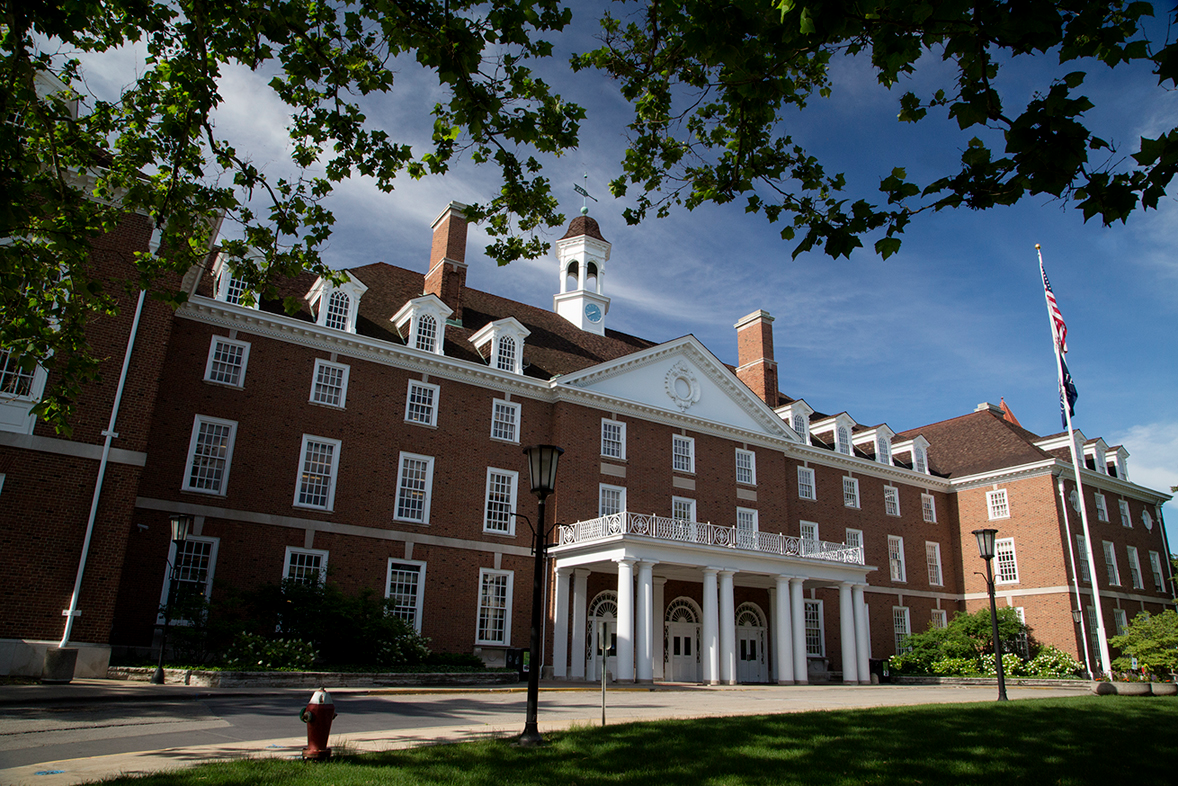
\includegraphics[scale=0.2]{illini-union.png}
	\end{subfigure}%
	\begin{subfigure}{0.5\textwidth}
		\centering
		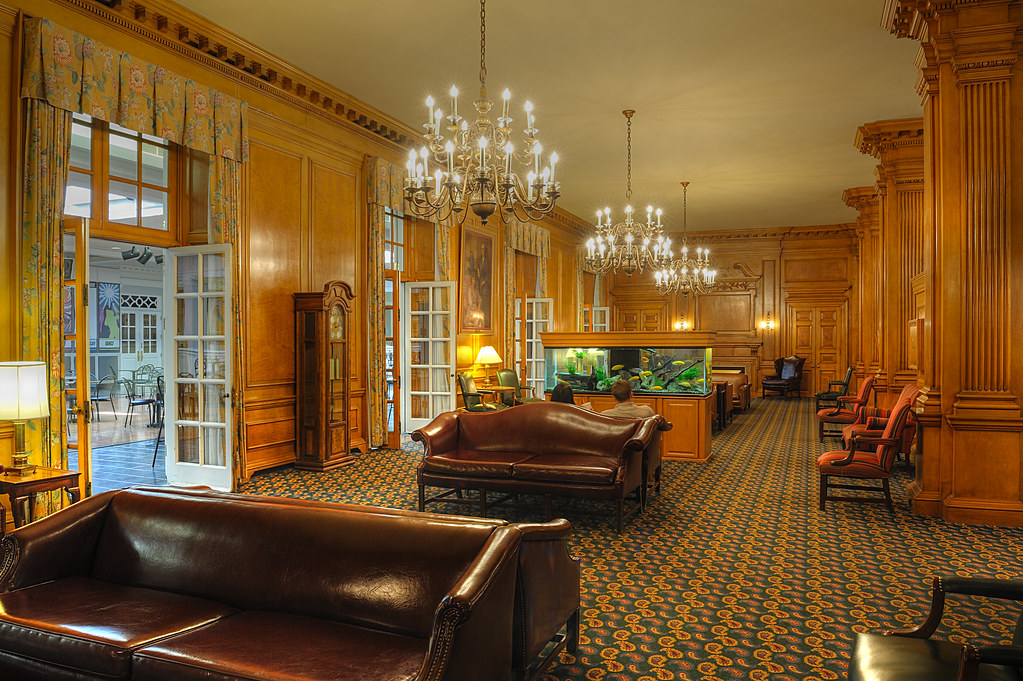
\includegraphics[width=0.9\linewidth]{union-inside.jpg}
	\end{subfigure}
	\caption{Illini Student Union}		
\end{figure} 


The Illini Union is capable of hosting the entire technical program of the ANS 
Student Conference. This keeps the conference contained in one convenient 
location while being within easy access of the rest of the campus. Technical 
sessions will be held in a combination of rooms on the second, third, and 
fourth floors of The Union. Each of these rooms have at least enough capacity 
for 42 people, lecture style, and A/V capability. There will also be rooms 
available to have panels and workshops during the course of the technical 
program. The Illini Rooms A and B will be a combined space for the career fair 
while Illini Room C and the south lounge will host the poster sessions. We will 
keep the space open to allow the poster sessions and career fair to share 
attendance and encourage networking. A detailed list of room capacities and 
floor plans are located in Appendix \ref{appendix:building}: Building Layout on 
page \pageref{appendix:building}.

\subsection{Banquet Space}
\subsubsection{Garden Hotel in Urbana}
The opening ceremony dinner on Thursday night will be hosted at the Garden Hotel in Urbana. It has a seating capacity of 600 people in round tables, offers in-house catering, and AV capabilities. This location was chosen for its convenience, as it would be the primary hotel for the conference. 

\begin{figure}[H]
    \centering
    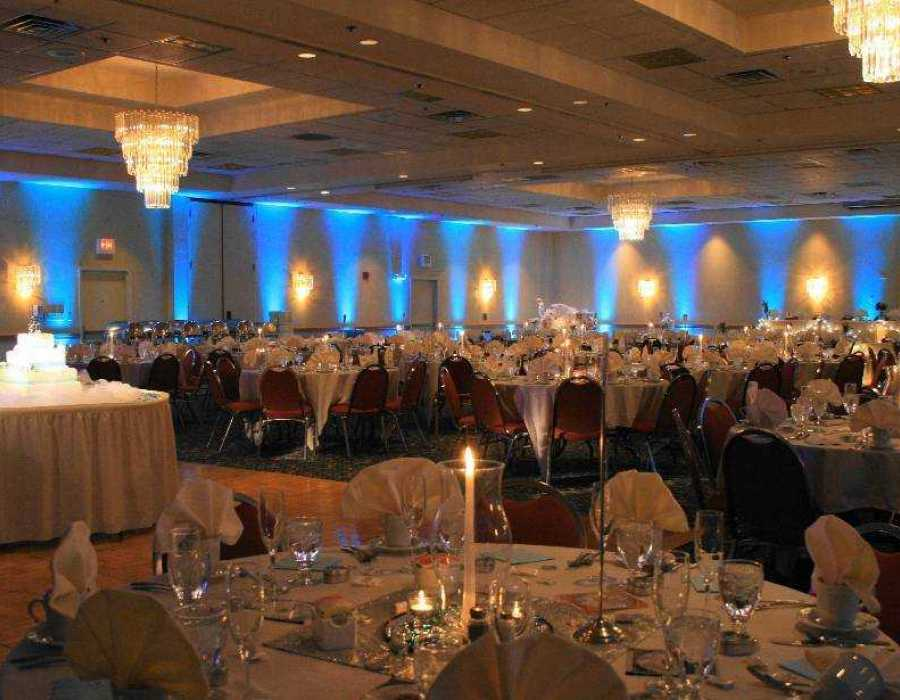
\includegraphics[width=0.35\textwidth]{garden_dinner.jpg}
    \caption{The Garden Hotel Banquet Hall with capacity for 600 people in round tables.}
\end{figure}

\subsubsection{I Hotel}
Dinner on Friday night will be hosted at the I Hotel. The I Hotel is undergoing an expansion that will increase the capacity of their banquet space to 690 people in rounds. Catering is provided by University Catering which avoids a 20\% gratuity charge because of its association with the University of Illinois. This expansion is set to be completed by Fall 2020. We will be hosting a social at the 77 Club in Memorial Stadium, which is just a brief walk up the street. Information about the I Hotel expansion is included in Appendix D. Cost of transportation to and from the I Hotel and 77 Club are discussed in the budget section.

\begin{figure}[H]
    \centering
    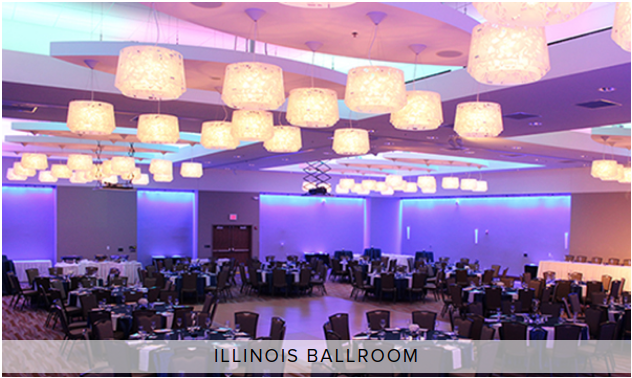
\includegraphics[width=0.5\textwidth]{ihotel-dinner.png}
    \caption{The current 400-person banquet space at the I Hotel is pictured 
        above. A new, 690-person ballroom will be available in 2020.}
\end{figure}

\subsubsection{Illini Union}
After the career fair is taken down on Saturday, the final dinner will be set up in the combined Illini Rooms, which has a seating capacity of 496 people in round tables. Catering will be provided by University Catering which allows us to avoid the 20\% gratuity for services. A floorplan for the Illini Rooms in round tables is available in \textbf{Appendix D}.\\


\begin{figure}[H]
    \centering
    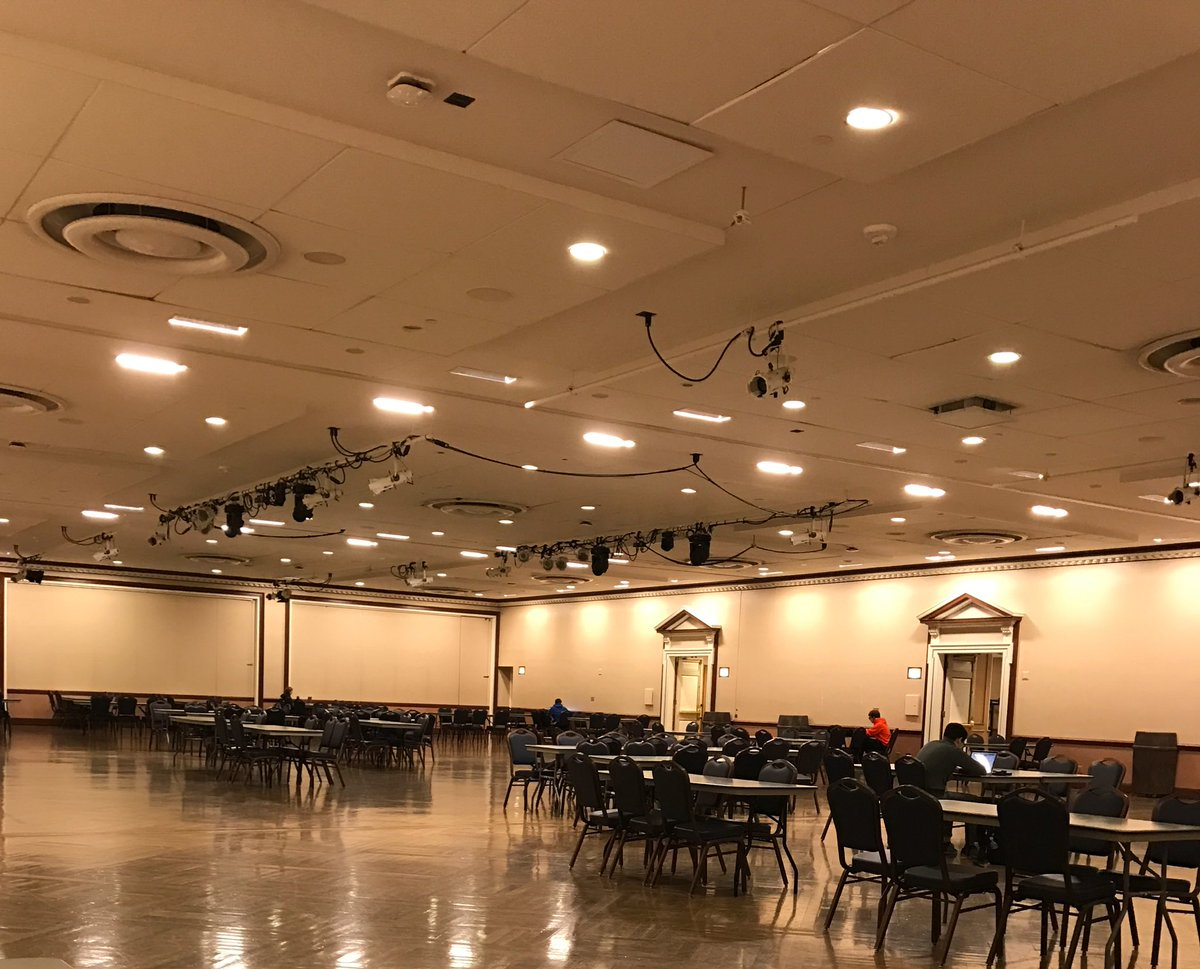
\includegraphics[width=0.75\textwidth]{illinirooms.jpg}
    \caption{The combined Illini rooms with capacity for 496 in round tables.}
\end{figure}


\subsection{Conference Contingency Plan}
In the event that the Union has reduced availability during the conference we have the ability to host technical sessions and workshops at a combination of buildings: The National Center for Supercomputing Applications (NCSA) and Beckman Institute. Rooms in Beckman Institute range from 20 - 60 classroom capacity. Most rooms have A/V capabilities. NCSA has rooms that can hold 13 - 50 people in lecture style. As these buildings are UIUC property, the cost of renting them are significantly reduced compared to a private facility. Additionally, these two buildings are adjacent to one another and are at most a 10 minute walk from the Union. We could also host all technical sessions at the I Hotel. Hosting at the I Hotel is more expensive than hosting in University buildings and would also require additional transportation options. We would need to reevaluate some parts of our budget in order to host the technical program at this venue. See Appendix E on page \pageref{appendix:map} for a map marking the locations of the proposed conference facilities.\\


\textbf{National Center for Supercomputing Applications (NCSA)}\\
NCSA is a hub of transdisciplinary research and digital scholarship where University of Illinois faculty, staff, and students, and collaborators from around the globe, unite to address research grand challenges for the benefit of science and society.\\
\begin{figure}[H]
	\centering
	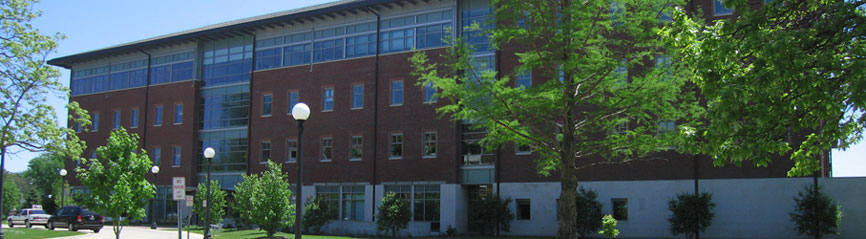
\includegraphics[width=0.8\textwidth]{ncsa_front.jpg}
	\caption{NCSA}
	\label{fig:ncsa}
\end{figure}

\textbf{Beckman Institute}\\
The Beckman Institute for Advanced Science and Technology at the University of Illinois is an interdisciplinary research institute devoted to leading-edge research in the physical sciences, computation, engineering, biology, behavior, cognition, and neuroscience.\\

\begin{figure}[H]
	\centering
	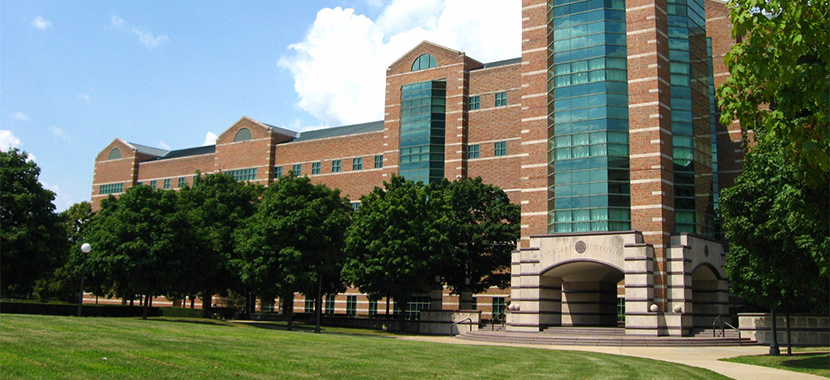
\includegraphics[width=0.8\textwidth]{beckman.jpg}
	\caption{Beckman Institute}
	\label{fig:beckman}
\end{figure}

\textbf{The I Hotel and Conference Center}\\
The I Hotel offers a unique, flexible, meeting space and a variety of small touches that make any meeting, social gathering or event in Champaign-Urbana a flawless and memorable experience.\\

\begin{figure}[H]
    \centering
    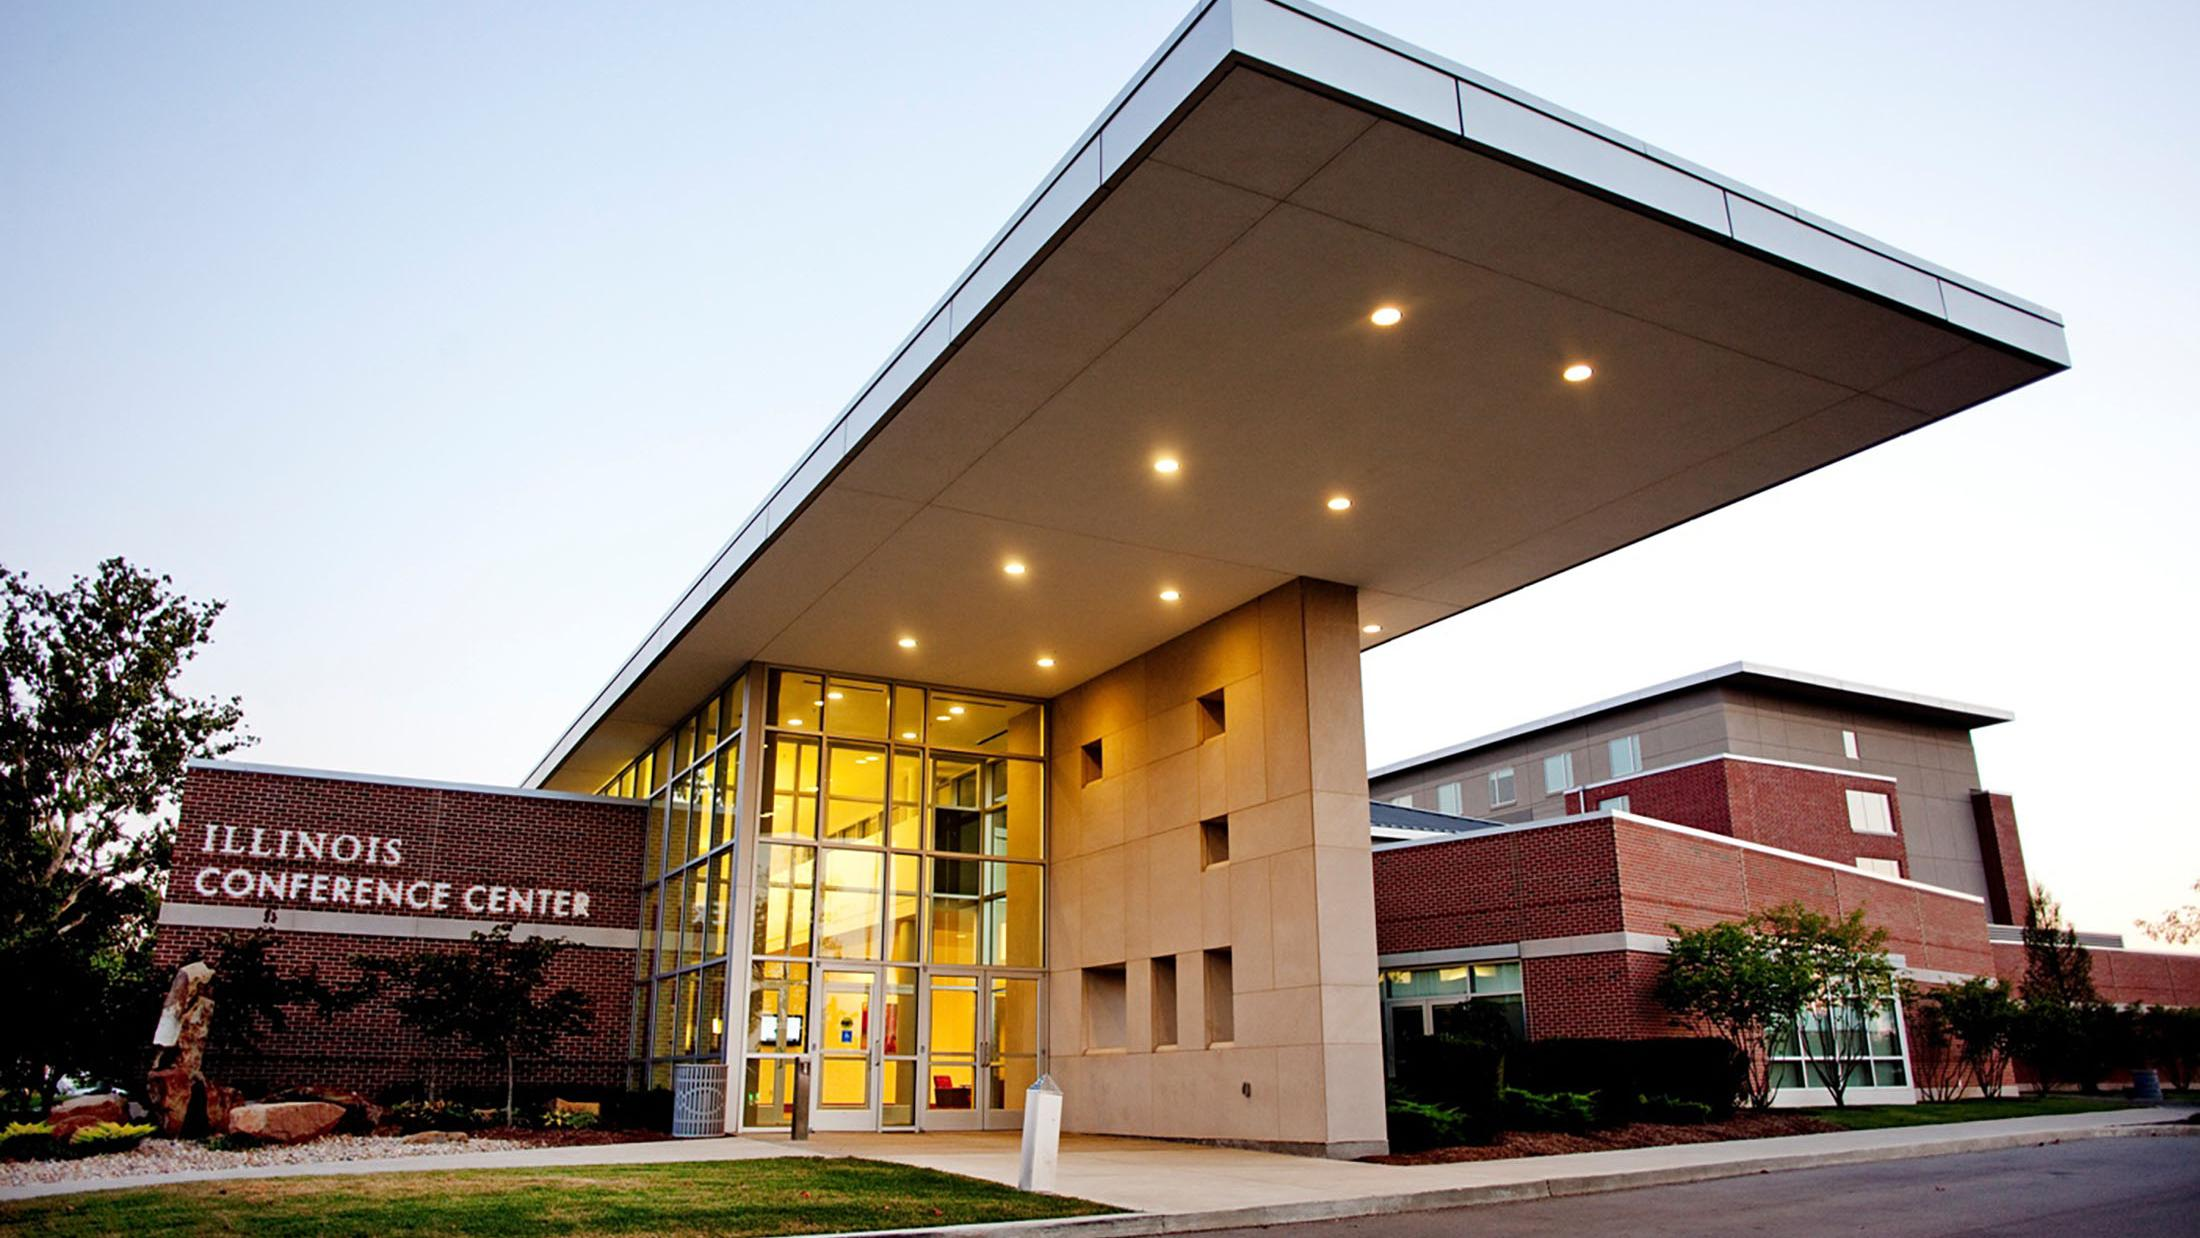
\includegraphics[width=0.8\textwidth]{ihotel.jpg}
    \caption{I Hotel}
    \label{fig:beckman}
\end{figure}

% \newpage
\subsection{Hotels and Accommodations}

$\textbf{The Garden Hotel Urbana}$\\
When selecting the primary hotel to accommodate students we considered the ability to host all students under one roof over proximity to the conference activities. The Garden Hotel Urbana (soon to be the Radisson) will be the primary hotel for all attendees. It features complimentary breakfast for its guests every morning. This will also be the location of the opening ceremony dinner. Since this hotel is just beyond walking distance from the main conference activities (2.2 miles), we will hire four Peoria Charter buses to shuttle attendees to and from the Union every 10 minutes. Additionally, there is a CU-MTD bus stop adjacent to the hotel that travels directly to the Union and runs every 10 minutes from 7am to 5am the following day for weekdays, and every 30 minutes on weekends.\\ 
\begin{figure}[H]
	\centering
	\begin{subfigure}{0.5\textwidth}
		\centering
		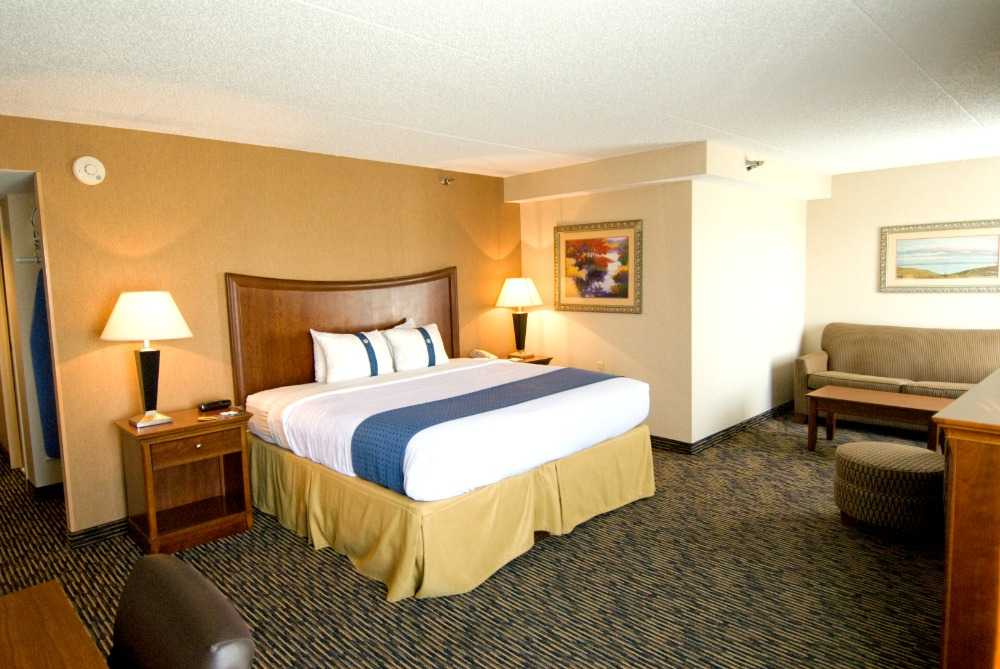
\includegraphics[width=0.9\linewidth]{garden_king.jpg}
		\subcaption{King Suite}
	\end{subfigure}%
	\begin{subfigure}{0.5\textwidth}
		\centering
		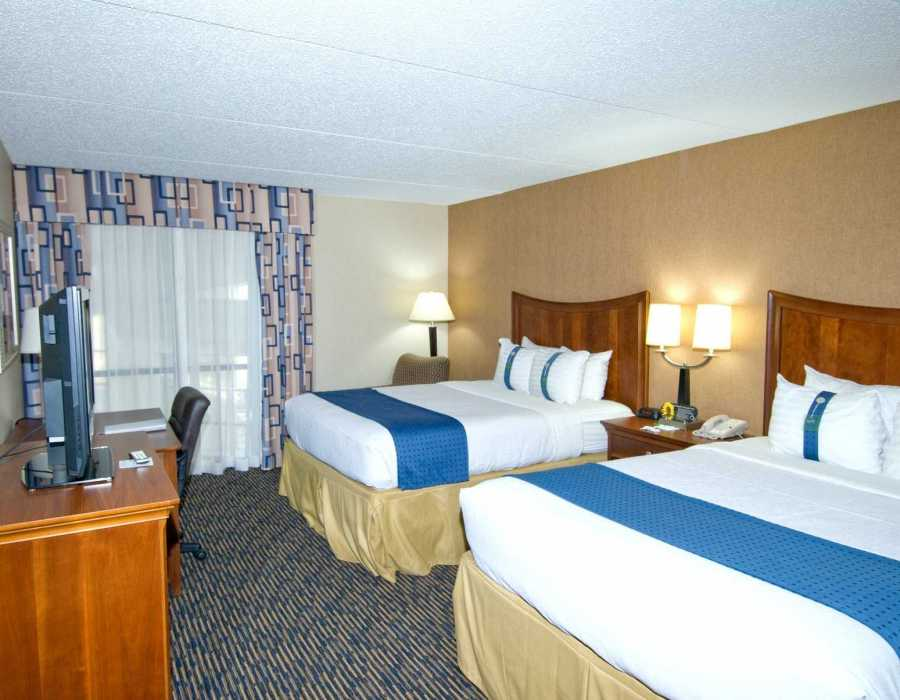
\includegraphics[width=0.9\linewidth]{garden_queen.jpg}
		\subcaption{Queen Double}
	\end{subfigure}
	\caption{Garden Urbana Hotel rooms}		
\end{figure} 

$\textbf{Illini Union}$\\
This is the primary hotel for invited speakers and panelists. Commuting to the conference will be as easy as taking the elevator downstairs because the Illini Union is where the primary conference activities will be held. The Union is also a five-minute walk from Green Street, the campus hub of dining and social activities. Guests have access to Wi-Fi and, upon request, guest passes to the university recreational facilities. Breakfast is provided in the form of vouchers for any of the hotel restaurant options inside the Union. Hosting technical sessions, workshops, and plenaries in the Union will help us negotiate a lower room rate.\\

\begin{figure}[H]
	\centering
	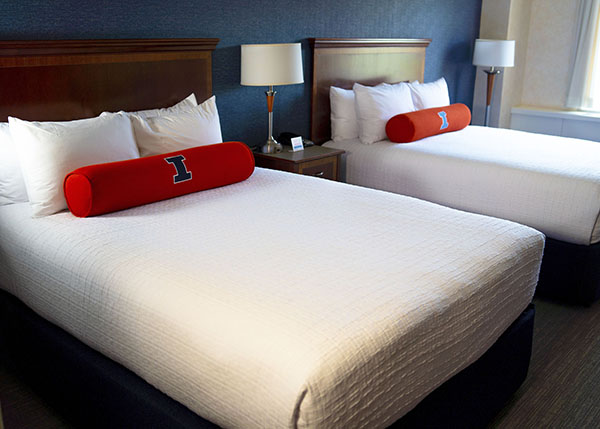
\includegraphics[width=0.35\linewidth]{illini-queen.jpg}
	\caption{Queen Double}		
\end{figure} 

$\textbf{Marriott TowneSuites}$\\
The Marriott TowneSuites is the professional's designated hotel; and, in the event that attendance exceeds 600 people, we will have overflow rooms in the Marriott TowneSuites. Rooms at the Marriott resemble a studio apartment with an open floor plan, refrigerator, stove, microwave,dishes, and dining area. Many rooms are equipped with pull-out couches, allowing 5 students to share a queen double room if desired. The hotel offers internet access for a maximum of 3 devices per room. The hotel is located on Green Street and the Illini Union a mere five-minute walk away. For $\$7$ a day, guests may park in a parking garage with 8ft clearance.\\

\begin{figure}[H]
	\centering
	\begin{subfigure}{0.5\textwidth}
		\centering
		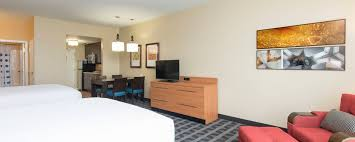
\includegraphics[width=0.75\linewidth]{marriott_room1.jpeg}
	\end{subfigure}%
	\begin{subfigure}{0.5\textwidth}
		\centering
		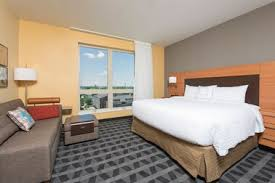
\includegraphics[width=0.75\linewidth]{marriott_room2.jpeg}
	\end{subfigure}
	\caption{Marriott Rooms: Left, a queen double. Right, a king single}		
\end{figure} 

UIUC is one of most well represented schools at past student conferences. Students from UIUC will be able to stay in their respective dorms and apartments to maximize the number of hotel rooms available to out of town guests. Sections seeking travel assistance are required to use the room blocks described above to prevent extra costs. Another proposed method to alleviate costs is to allow an option for students from smaller sections to be housed at an ANS-UIUC section member's apartment. The Diversity co-chair will assume responsibilities of reaching out to members-at-large and other minority serving institutions. 


\begin{table}[H]
\caption{Cost of Hotels}
\label{table:hotels}
	\centering
	\makebox[0.6\linewidth]{\begin{tabular}{lccccc}
	\hline\hline
	\textbf{Hotel} & \textbf{Distance from} & \textbf{Dates} & \textbf{Number of Rooms} & \textbf{Rates*} & \textbf{Per Person**}\\
                & \textbf{the Union (mi)} & & & & \\
	\hline\hline
	Garden Urbana & 2.2  & 4/8-4/11 & 198 & 119 & $\$$29.75\\
	Illini Union & 0.0 & 4/8-4/11 & 35 & 134 & $\$$33.5\\
	Marriott TowneSuites &0.25 & 4/8-4/11 & 95 & 189 & \$47.50\\ 
	\hline
	\end{tabular}}
\subcaption*{\textbf{*}\textit{Price for a queen double}\\ \textbf{**}\textit{Assumes 4 people per room}}
\end{table}

\subsection{Dining}
\subsubsection{Breakfast}
Our primary hotel, the Garden Hotel in Urbana, soon to be the Radisson Hotel, serves complimentary breakfast every morning. Due to this, we will not be catering breakfast at the Illini Union during the conference. Guests staying at the Illini Union Hotel are provided with vouchers for breakfast at the food court in the basement of the Union. The food court offers Einstein Bros, Starbucks, Garbanzo Mediterranean, and more. 
\subsubsection{Lunch}
Conference attendees are encouraged to explore the University’s campus and surroundings, including getting lunch on the main street of campus, Green street. Due to this, lunch will not be provided for the conference. However, box lunches will be provided for the Student Sections Committee meeting from 11:30pm to 1:30pm on Friday as well as any lunch and learns hosted by sponsors on Friday and Saturday. The Illini Union’s catering service, University Catering, will be used. Sponsors can also choose to sponsor and host a lunch in one of the technical session rooms on Friday or Saturday. If more rooms are required, there are available rooms on the first and second floor of the Union. Sponsors will be able to use University Catering, or cater from one of the food vendors in the Illini Union.
\subsubsection{Dinner}

\textbf{Thursday Night}\\
Communicating the science of nuclear energy remains one of the chief challenges of our field. The opening dinner of this conference will focus on science communication and the people behind the science. Science communication requires more than the recitation of raw data to be effective. By telling our own, diverse backstories, we become more effective science communicators. Speakers will be asked to speak to their own backstory as a nuclear advocate and how their story makes them a more effective communicator.\\\\
\indent\textbf{Friday Night}\\
The second dinner will be themed around networking and professional-development and how these critical tools have value beyond finding jobs. Communities like ANS thrive on the exchange of ideas and knowledge. The student conference serves plays an essential role by connecting the burgeoning minds of the next generation with the wisdom of established professionals. This dinner will consist of tables organized by company/national laboratory or by topic/discipline area to allow students and professionals to mingle, promoting the exchange of ideas.\\\\ 
\indent\textbf{Saturday Night}\\
The closing dinner of the conference will be a call to action for student attendees. Ours is a generation faced with challenges on a scale never witnessed by humanity, and we will only successfully address these challenges through the engagement of as many bright young minds as possible. The speakers for this night will be asked to address ways we all can take individual responsibility for the grand challenges of our age by using our own unique skills to tackle problems like climate change and energy poverty from every angle imaginable.\\ 
\subsection{Travel and Transportation}

\subsubsection{Getting to Champaign}
The University of Illinois is a 2.5 hour drive from one of the largest airports in the world, O'Hare International Airport. There is also a small airport located just 20 minutes outside of campus. Additionally, there is a reliable bus service, Peoria Charter, that runs between O'Hare and the UIUC campus several times per day. Table \ref{table:airfare} shows the round-trip, non-stop, airfare costs for the first weekend of April. Peoria Charter fare from O'Hare to UIUC is currently $\$61$ round-trip. While travel from airport to hotel can be managed by train (Amtrak/Metra), the conference planning committee excluded this option due to the added complexities of getting from the airport to train station, and train station to hotel with the associated costs of doing so. We believe the charter bus to be the best route of action as it picks up travelers directly at the arrivals gate and brings them to the Illini Union. Due to the central location of UIUC, driving might be a good option for some schools and individuals. Table \ref{table:ground} shows the approximate driving times and costs from several universities. 

\begin{table}[H]
\caption{Estimated Costs of Ground Travel}
\label{table:ground}
   \begin{tabular}{lcccc}
   \hline\hline
   \textbf{School}&\textbf{Estimated Mileage (mi)}&\textbf{Driving Time (hrs)}&\textbf{Fuel Cost*}&\textbf{Per Person**}\\
   \hline\hline
    Purdue University&90&1h 40m&\$21.86&\$5.47\\
    University of Cincinnati&233& 3h 40m&\$56.60&\$14.15\\
    Air Force Tech &250&3h 58m&\$60.73&\$15.18\\
    University of Wisconsin&253&4h&\$61.46&\$15.36\\
    Missouri University S \& T &279&4h 21m&\$67.77&\$16.94\\
    U. Missouri - Columbia&291&4h 28m&\$70.69&\$17.67\\
    Ohio State University&302&4h 47m&\$73.36&\$18.34\\
    University of Michigan&345&5h 17m&\$83.81&\$20.95\\
    Vanderbilt University&373&5h 33m&\$90.61&\$22.65\\
    Iowa State University&378&5h 44m&\$91.82&\$22.96\\
    \hline
    Average&279&4h 22m&\$67.87&\$16.97

    \end{tabular}
\subcaption*{\textbf{*}\textit{Estimated assuming an average 23 MPG} \textbf{**}\textit{Assumes four people in a car}} 
\end{table}


\subsubsection{Getting to the Conference}
% The primary hotel, Garden Hotel Urbana, is approximately two miles from the Union and outside of reasonable walking distance. Thus we have budgeted to include transportation provided by Peoria Charter. We intend to have busses shuttling continuously between the Union and the Garden Hotel Urbana. For those who desire more flexibility and freedom, there is CU-MTD bus stop adjacent to the hotel that has a bus every 10 minutes. This bus route, the 22 Illini, can take attendees directly to the Union from the hotel. It is also one of the main campus bus routes and can take travelers almost anywhere on or around campus. Lyft and Uber are available as well for attendees that choose to use those services. A map of the bus route is in Appendix E: Campus Map of Locations on page \pageref{appendix:map}.
Each day of the conference, there will be four, 55 passenger, busses from Peoria Charter outside the hotel by 7:00 AM. They will leave as they fill up and be staggered such that there will be two busses arriving at either the Union or the hotel every ten minutes. These busses will run throughout the day from 7:00 AM to 5:00 PM. At 5:00 PM the busses will begin transporting attendees to the dinner venue (except on Thursday night when the dinner is located at the Garden Hotel) until 6:00 PM. Busses will be available at 8:00 PM until 9:00 PM to transport attendees either back to the hotel or to the evening social. The final rounds of busses will be optionally available to take attendees from the social to the hotel at 10pm. For those who desire more flexibility and freedom, there is CU-MTD bus stop adjacent to the hotel that has a bus every 10 minutes. This bus route, the 22 Illini, can take attendees directly to the Union from the hotel. It is also one of the main campus bus routes and can take travelers almost anywhere on or around campus. Lyft and Uber are available as well for attendees that choose to use those services. A map of the bus route is in Appendix E: Campus Map of Locations on page \pageref{appendix:map}.
\begin{figure}[H]
	\centering
	\label{figure:busses}
	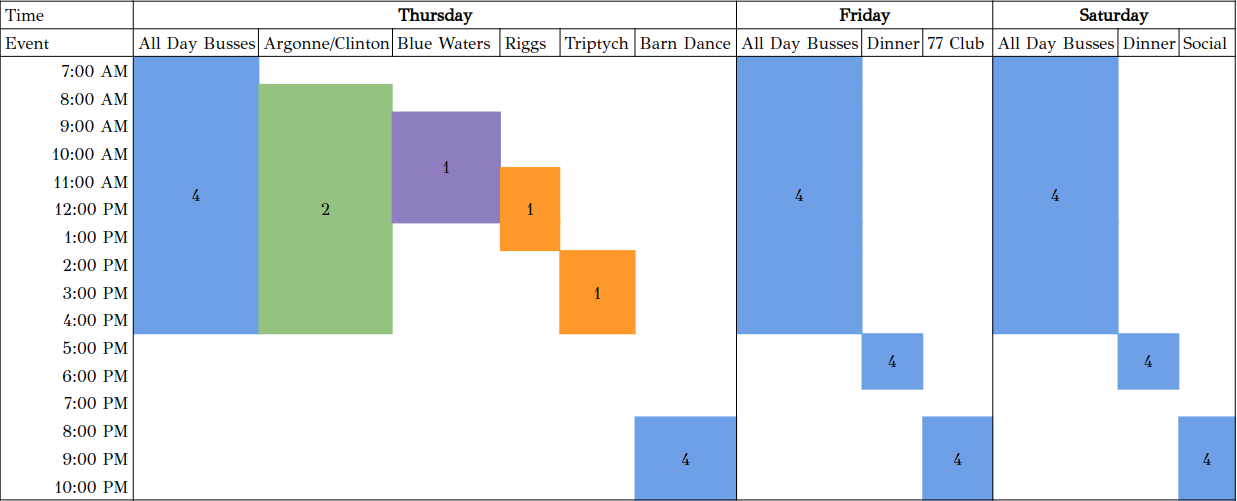
\includegraphics[scale=0.3]{transportation.png}
	\caption{Summary of Bus Transportation}
	\subcaption*{Same color refers to same set of busses.}
\end{figure}




\begin{table}[H]
\caption{Airfare to Chicago/Champaign}
\label{table:airfare}
   \begin{tabular}{lccc}
   	\hline\hline
    \textbf{School} & \textbf{Departure City} & \textbf{O'Hare (ORD)*} & \textbf{Willard (CMI)} \\
    \hline\hline
    University of California - Berkeley & San Francisco (SFO) & $\$$338 & $\$$436 \\
    University of California - Irvine&Orange County (SNA)&$\$$394&$\$$436\\
    Colorado School of Mines & Denver (DEN) & $\$$222 & $\$$328 \\
    Three Rivers Community College & Hartford (BDL) & $\$$468 & $\$$327 \\ 
    University of Florida & Gainesville (GNV)& $\$$377 & $\$$416 \\
    Georgia Institute of Technology & Atlanta (ATL)& $\$$199 & $\$$291 \\
    Southern Polytechnic State University & Atlanta (ATL) & $\$$199 & $\$$291 \\
    Idaho State University & Idaho Falls (IDA) & $\$$501 & NA \\
    Kansas State University & Manhattan (MHK) & $\$$336 & $\$$406 \\ 
    Louisiana State University & Baton Rouge (BTR) & $\$$380 & $\$$329 \\
    United States Naval Academy & Hanover (BWI) & $\$$210 & $\$$321 \\  
    University of Maryland & Hanover (BWI)&$\$$210 &$\$$321 \\ 
    Massachusetts Institute of Technology & Boston (BOS)&$\$$191 &$\$$325 \\ 
    University of Massachusetts - Lowell &Boston (BOS) &$\$$191 &$\$$325 \\
    University of Nevada - Las Vegas & Las Vegas (LAS)& $\$$262 &$\$$358 \\ 
    University of New Mexico &Albuquerque (ABQ) &$\$$439 &$\$$358 \\ 
    City College of New York &\$New York (JFK) &$\$$245 &$\$$325 \\
    Excelsior College & Albany (ALB) &$\$$444 &$\$$327 \\ 
    Rensselaer Polytechnic Institute & Albany (ALB)&$\$$444 &$\$$327 \\ 
    United States Military Academy at West Point&New Windsor (SWF)&$\$$273 &$\$$357 \\ 
    North Carolina State University &Morrisville (RDU) &$\$$180 &$\$$321 \\
    Oregon State University &Portland (PDX) &$\$$314 &$\$$436 \\ 
    Pennsylvania State University & Harrisburg (MDT)&$\$$397 & $\$$323 \\
    University of Pittsburgh &Pittsburgh (PIT) &$\$$282 &$\$$293 \\ 
    Clemson University&Greenville (GSP)&$\$$356&$\$$287\\
    South Carolina State University&Columbia (CAE)&$\$$407 &$\$$564 \\ 
    University of South Carolina&Columbia (CAE)&$\$$407&$\$$564\\
    Chattanooga State Comunity College&Chattanooga (CHA)&$\$$334&$\$$316\\
    University of Tennessee&Knoxville (TYS)&$\$$340&$\$$291\\
    Texas A\&M University&College Station (CLL)&$\$$367&$\$$243\\
    University of Texas - Arlington&Dallas (DFW)&$\$$197&$\$$303\\
    University of Texas - Austin&Austin (AUS)&$\$$298&$\$$358\\
    University of Texas - Permian Basin&Midland (MAF)&$\$$434&$\$$333\\
    Utah State University&Salt Lake City (SLC)&$\$$298&$\$$358\\
    University of Utah&Salt Lake City (SLC)&$\$$298&$\$$358\\
    Virginia Commonwealth University&Richmond (RIC)&$\$$279&$\$$321\\
    University of Washington&Seattle (SEA)&$\$$253&$\$$436\\
    \hline
    Average Lowest Cost for Air Travel**&$\$$293&&
    \end{tabular} 
\end{table}

\noindent\textbf{*}\textit{A \$61 round-trip bus ticket through Peoria Charter was added to the cost.}\\
\textbf{**}\textit{The average of the lowest price between O'Hare and Willard.}\\



\newpage
\section{Conference Program}

% Request review from Katy Huff
\subsection{Potential Speakers}

\subsubsection{Rita Baranwal, DOE Nuclear Energy}
\setlength\intextsep{0pt}
\begin{wrapfigure}{R}{0.25\textwidth}
	\begin{center}
		% \vspace{-\baselineskip}
		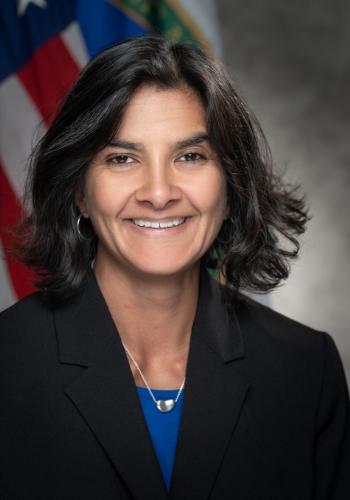
\includegraphics[height=13\baselineskip]{fmt-baranwal.jpg}
	\end{center}
\end{wrapfigure}
Dr. Rita Baranwal serves as the Assistant Secretary for the Office of Nuclear Energy in the U.S. Department of Energy (DOE).  Dr. Baranwal leads the office’s efforts to promote research and development (R$\&$D) on existing and advanced nuclear technologies that sustain the existing U.S. fleet of nuclear reactors, enable the deployment of advanced nuclear energy systems, and enhance the U.S.A.'s global commercial nuclear energy competitiveness. Prior to her current role, Dr. Baranwal directed the Gateway for Accelerated Innovation in Nuclear (GAIN) initiative at Idaho National Laboratory.  She was responsible for providing the nuclear industry and other stakeholders access to DOE's state-of-the-art R$\&$D expertise, capabilities, and infrastructure to achieve faster and cost-effective development, demonstration, and ultimate deployment of innovative nuclear energy technologies. Under her leadership, GAIN positively impacted over 120 companies. Baranwal is a clear choice of speaker to discuss the ways to improve nuclear legislation and how companies can rapidly develop new nuclear technology.\\

\clearpage
\subsubsection{Rachel Slaybaugh, UC Berkeley}
\setlength\intextsep{0pt}
\begin{wrapfigure}{l}{0.25\textwidth}
	\begin{center}
		% \vspace{-\baselineskip}
		
\includegraphics[height=13\baselineskip]{fmt-slaybaugh.jpg}
	\end{center}
\end{wrapfigure}
Prof. Slaybaugh's research is based in numerical methods for neutron transport with an emphasis on supercomputing. She applies these methods to reactor design, shielding, and nuclear security and nonproliferation. Slaybaugh was a key founder of the nuclear innovation bootcamp, which seeks to train students and professionals in skills essential to innovation in nuclear energy while executing team projects. Finally, Slaybaugh has served as a Program Director at ARPA-E, developing and running their first fission energy programs. Advanced Research Projects Agency-Energy (ARPA-E) invests in research for ways to generate, use, and store energy. These projects have the potential to radically improve economic prosperity in the U.S. and environmental wellbeing. Due to her endeavors in teaching and sharing nuclear innovation, we believe that Slaybaugh's goals are aligned with the goals of this conference and would make her an excellent addition to the program. Slaybaugh has much to offer the conference with her vision and leadership.\\


\subsubsection{William Magwood}
\setlength\intextsep{0pt}
\begin{wrapfigure}{R}{0.25\textwidth}
	\begin{center}
		% \vspace{-\baselineskip}
		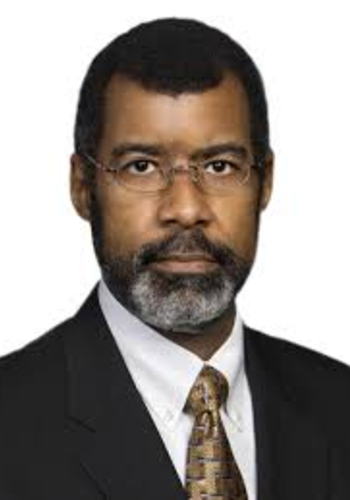
\includegraphics[height=13\baselineskip]{fmt-magwood.jpeg}
	\end{center}
\end{wrapfigure}
Mr. Magwood served seven years as the Director of Nuclear Energy with the U.S. Department of Energy (DOE), where he was the senior nuclear technology official in the United States Government. He oversaw the restoration of the Federal nuclear technology program and led the creation of ``Nuclear Power 2010,'' ``Generation IV,'' and other innovative initiatives—including successful efforts that helped reverse the decline in American nuclear technology education. Since joining the NRC, he has continued his advocacy for both U.S. science and technology education and strong international cooperation. He has also sought to assure transparency and improve the agency's openness to public participation. As an NRC Commissioner, Mr. Magwood has been a strong defender of the NRC's regulatory independence and adherence to the principle that regulations should be based firmly on scientific and technical facts. From his nomination as a Commissioner, Mr. Magwood has remained committed to his promise to carry out his responsibilities ``in a manner that earns the public's trust, and always doing the right thing even when the right thing isn't easy.''

\subsubsection{Phi Nguyen, Former Vice President and Director of Engineering at Intel}
\setlength\intextsep{0pt}
\begin{wrapfigure}{l}{0.25\textwidth}
	\begin{center}
		% \vspace{-\baselineskip}
		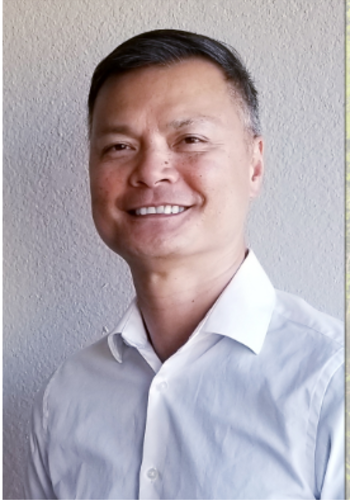
\includegraphics[height=13\baselineskip]{fmt-nguyen.png}
	\end{center}
\end{wrapfigure}
Phi Nguyen, is a UIUC alumni from the NPRE department and went on to a major leadership role at the Intel corporation. Smartphones, computers, and other technology that most Americans take for granted everyday would not be possible without innovations from companies like Intel. Plasma processing plays a significant role in the production of key components of these devices. As the former Director of Engineering at Intel, Phi Nguyen is the perfect person to talk about how this important research helps solve big problems. 
\clearpage

\subsubsection{Suzanne Hobbs Baker}
\setlength\intextsep{0pt}
\begin{wrapfigure}{R}{0.25\textwidth}
	\begin{center}
		% \vspace{-\baselineskip}
		
\includegraphics[height=13\baselineskip]{fmt-baker.jpeg}
	\end{center}
\end{wrapfigure}
Talking about nuclear energy, specifically with the general public, is one of Suzanne Hobbs Baker's key goals. Baker has a strong track record as a nuclear science communicator. In 2008 she founded a nonprofit organization aimed at reaching women, minorities, and young people with critical information about climate change and nuclear energy. She currently works as the creative director for Fast Path to Zero Initiatve at the University of Michigan and as a Nuclear security fellow with Third Way Energy. Baker's work in empowering minorities and students to solve the world climate crisis with nuclear energy, as well as her skill in creative science communication, ensures that Baker has a lot to offer the student conference. Celebrating the people behind the science is one of the key goals of this conference and an area in which Baker has a lot of experience.\\

% \newline
% \vspace{2cm}
% \newline
\subsubsection{Todd Allen, UW Madison}
\setlength\intextsep{0pt}
\begin{wrapfigure}{l}{0.25\textwidth}
	\begin{center}
		% \vspace{-\baselineskip}
		
\includegraphics[height=13\baselineskip]{fmt-allen.jpeg}
	\end{center}
\end{wrapfigure}
His first post-Ph.D. position was as a staff scientist at Argonne National Laboratory. While at Argonne, he joined the leadership team tasked with developing the Generation IV Roadmap, the document that framed the resurgence of the nuclear research programs early in the 21st Century.Following Argonne, he joined the faculty at the University of Wisconsin. While there, he split his time between establishing a premier material science program at the university and supporting the Idaho National Laboratory. At INL, he led the transition of the Advanced Test Reactor into a national user facility. He also ran a six-institution Energy Frontier Research Center focused on answering fundamental questions about heat transfer in nuclear fuel.
From 2013-2016, he helped lead the Idaho National Laboratory as the Deputy Laboratory Director for Science $\&$ Technology, including being an important contributor to the development of the Gateway for Accelerated Innovation in Nuclear (GAIN) initiative announced at the White House in November 2015. Since 2016 he has been a Visiting Senior Fellow with Clean Energy Program at Third Way, a Washington, DC based think tank. His role in formulating the roadmap for Generation IV reactors and his leadership indicate that he would make a great speaker at the conference.\\

% \clearpage
\subsubsection{Jim Conca, Forbes}
\setlength\intextsep{0pt}
\begin{wrapfigure}{R}{0.25\textwidth}
	\begin{center}
		% \vspace{-\baselineskip}
		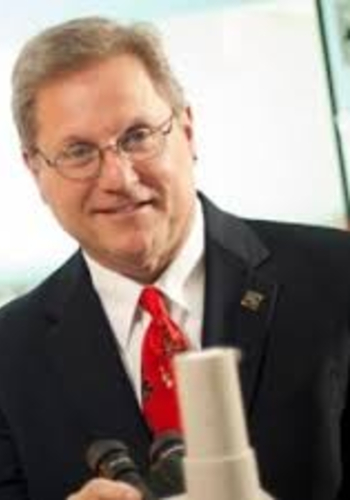
\includegraphics[height=13\baselineskip]{fmt-conca.jpeg}
	\end{center}
\end{wrapfigure}
Jim Conca has been a scientist in the field of the earth and environmental sciences for 33 years, specializing in geologic disposal of nuclear waste, energy-related research, planetary surface processes, radiobiology and shielding for space colonies, subsurface transport and environmental clean-up of heavy metals. He is a Trustee of the Herbert M. Parker Foundation, Adjunct at WSU, an Affiliate Scientist at LANL and consult on strategic planning for the DOE, EPA/State environmental agencies, and industry including companies that own nuclear, hydro, wind farms, large solar arrays, coal and gas plants. He also writes for Forbes magazine about nuclear issues, energy, and the environment. Conca has a strong vision for the future and is not shy about coming up with ideas to solve grand challenge problems. In addition to his experience and ambition, he is an excellent science communicator to scientists and non-scientists alike. Together, these factors make him an ideal speaker at the conference.

% \clearpage
\subsubsection{Ross Radel, CEO Phoenix, LLC}
\setlength\intextsep{0pt}
\begin{wrapfigure}{l}{0.25\textwidth}
	\begin{center}
		% \vspace{-\baselineskip}
		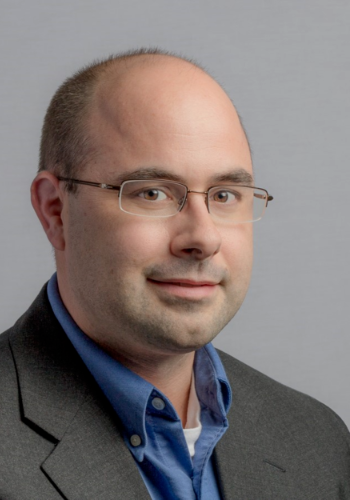
\includegraphics[height=13\baselineskip]{fmt-radel.png}
	\end{center}
\end{wrapfigure}
Ross is the CEO and a Board of Directors member of Phoenix. He holds a MS and a PhD in Nuclear Engineering from the University of Wisconsin-Madison. He previously worked as the Senior Member of the Technical Staff at Sandia National Laboratories. Ross has extensive experience with nuclear reactors and advanced power conversion systems that are directly applicable to Phoenix’s core technologies. His previous research at the University of Wisconsin focused on high-flux neutron generation for detecting clandestine material, specifically highly enriched uranium. The mission of Radel's company, Phoenix, is to transform nuclear technology to better our world. This mission statement reflects our mission in hosting the student conference well. We believe Dr. Radel would be a great speaker for the future of nuclear technology.\\


\subsubsection{Greg Piefer, CEO SHINE}
\setlength\intextsep{0pt}
\begin{wrapfigure}{R}{0.25\textwidth}
	\begin{center}
		% \vspace{-\baselineskip}
		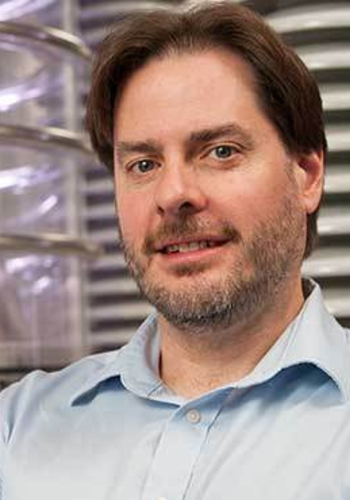
\includegraphics[height=13\baselineskip]{fmt-piefer.jpg}
	\end{center}
\end{wrapfigure}
Dr. Piefer is the founder and CEO of SHINE Medical Technologies. The mission of SHINE is to lead the world in safe, clean, and affordable production of medical tracers and treatment elements. He holds a PhD in nuclear engineering, and BS degrees in physics and electrical and computer engineering from the University of Wisconsin–Madison. Greg has received numerous awards and honors including the prestigious UW-Madison Early Career award, is the primary inventor on multiple patents and author or co-author of numerous publications, and serves on the boards of several profit and non-profit entities. His passion is the growth of technology companies that take scientific advancement to commercialization, providing the opportunity to serve and better humanity. Piefer's goals are perfectly attuned to the goals of this conference and he would be an excellent speaker on the powerful applications of radiological engineering.\\

\subsection{Saving the World Panel Series}
Technical and non-technical panels encourage interaction between students and professionals at the conference. Each panel is designed to address one or more of the stated goals for the conference. They also serve as a way for students and professionals to learn more about relevant issues, find inspiration for their next project, and feel encouraged for the future of the nuclear field.\\
 
$\Large\textbf{Technical Panels}$

\subsubsection{Critical Conversations: Microreactors}
Microreactors are a growing area of nuclear research and the first installations have been projected for some time in the mid 2020s. They are capable of generating 1-50 MWth, which can be used directly or converted to electricity. These relatively portable reactors are capable of powering remote areas and towns with little infrastructure. UIUC has stated that it aims to be carbon neutral by 2050. The University is exploring the possibility of constructing a microreactor on campus for research and power generation, a first of its kind, in pursuit of its decarbonization goals. This panel will discuss the benefits and applications for microreactors around the world and also talk specifically about the potential market for microreactors on universities. We have a several groups on campus researching, simulating, and modelling microreactors. Faculty leading these groups would be excellent speakers on this panel.


\subsubsection{Applications for Plasma Processing}
Plasma processing has become a staple in many fields of advanced manufacturing. Without plasma, modern conveniences such as smartphones and powerful computer technology would not be possible. In this panel, representatives from companies at the cutting-edge of plasma processing research will discuss how plasmas continue to revolutionize contemporary industry. Potential panelists include Brian Jurczyk, CEO of Starfire Industries, and Phi Nguyen, former Vice President and Director of Engineering at Intel Corp.

\subsubsection{Fusion: Materials for the Future}
Nuclear fusion has the potential to serve as the ultimate clean energy source, capable of supplying the world’s energy needs for millennia. Harnessing this immensely powerful energy resource requires further innovation in a variety of scientific disciplines. One of the largest remaining obstacles to fusion energy is the unprecedented strain placed on the materials from which fusion reactors are built. This panel will focus on the latest advancements in plasma facing components research and could feature panelists such as Professor David Ruzic, director of the UIUC Center for Plasma-Material Interactions, and Dr. Lauren Garrison, Weinberg Fellow at ORNL.

\subsubsection{Nuclear Policy and Legislation}
Nuclear energy is one of the most heavily regulated fields in the United States. This panel aims to enlighten attendees about how legislation is written and how non-scientist government officials might better understand the potential of nuclear energy. This panel will allow attendees to learn who is working in this area and develop a network of people devoted to issues of nuclear policy.
Rita Baranwal would be an excellent speaker on this panel because of her work for the DOE.

\subsubsection{Radiological Techonology for a Healthier and Safer Future}
From the production of medical isotopes to nuclear verification, radiological engineering will play an important role in the future of health, security, and more. This panel will illuminate some of those applications and show attendees what could be possible with radiological technology. Speakers may include Greg Piefer from SHINE and Ross Radel from Phoenix.\\

$\Large\textbf{Non-Technical Panels}$

\subsubsection{Science is People: Conducting Inclusive Research}
Research and technology that will help us solve the grand challenge problems of the world must also reflect the diverse needs of the people that live in it. Everyone comes to nuclear engineering from a variety of backgrounds, identities, abilities, and experiences. Saving the World One Atom at a Time means making atomic contributions. Finding ways to encourage and include even one more person in the endeavor of nuclear science is an important kind of atomic contribution. This panel works toward the goal of celebrating the people behind the science. It also serves to inspire students and 

\subsubsection{Talking To Non-Scientists}
It has been shown that when members of the general public are given more scientific evidence they are less likely to shift their beliefs. While this finding is surprising to members of the scientific community, people who value data and evidence, it can be difficult to find ways to effectively communicate your research to the public. Attendees will learn how other scientists effectively communicate their results. No longer discouraged by potential resistance from the public, students will steel their resolve for working on ambitious projects that can save the world. Suzanne Hobbs Baker would be a great choice for this panel, as well as members of The Story Collider; a non-profit organization devoted to helping scientists tell stories that 

\subsubsection{How to Host a Conference}
This panel is devoted to sharing the experience of this conference's planning committee with students from other schools that may want to host their own student conference. This panel is for students by students. We will discuss our process from writing a successful proposal to executing a successful conference. 


\subsection{Workshops}

\subsubsection{Scientific Storytelling}
Science is people. The Story Collider is a non-profit organization whose mission is to honor the people and stories behind the science and teach scientists to use these stories to their advantage. From their website:
\begin{quote}
	We know that storytelling is not typically taught during scientific training, and is sometimes explicitly discouraged. There are many reasons why. But like it or not, stories are how people understand the world, and they weave together fact and emotion. Compared to other forms of communication, these narratives can be more successful in:
	\begin{itemize}
		\item generating interest and engagement with a topic,
		\item improving comprehension, and
		\item influencing real-world beliefs, even among skeptical audiences.
	\end{itemize}
\end{quote}

\subsubsection{Building Your Network}
The AAAS conducts workshops that teach early career scientists and students how to develop a professional network that will benefit them in the future. They hold regular workshops about strategic networking, making new contacts, and getting the most out of a conference. We will invite them to conduct a workshop where attendees can come away with skills to maximize their experience at the ANS Student Conference.

\subsubsection{MOOSE Workshop}
The Multiphysics Object Oriented Simulation Environment is an open source framework for finite element modeling, developed and maintained by Idaho National Laboratory. MOOSE is a powerful framework that enables users to couple several different physics codes together under a single API. Many research groups at UIUC use this framework for simulating reactors and materials. The Idaho National Laboratory MOOSE team gives many workshops a year to train future user-developers of the framework. We will invite this team to give a half-day MOOSE workshop at the conference. The workshop will take place in NCSA room 1030.

\subsubsection{PyNE and PyRK Workshop}
Python for Nuclear Engineering (PyNE) and Python for Reactor Kinetics (PyRK) are two open source packages with computational tools for nuclear science and engineering. The PyNE toolkit provides both a Python and a C++ API for common computational pre- and post-processing tasks in nuclear engineering. PyRK offers point kinetics implementation for nuclear reactors. This workshop will provide a hands-on tutorial for attendees to begin using PyNE and make use of its capabilities for their curriculum and research work. The Advanced Reactors and Fuel Cycles (ARFC) research group at UIUC and its collaborators will provide instructors. This workshop, alpha-tested at the University of Wisconsin will be aimed at students who can provid their own laptops and have a desire to improve their nuclear computational skills. The workshop will be approximately two hours of instruction at NCSA room 1030.


\subsection{Technical Sessions}

Technical sessions are an integral part of every student conference. This is where students can share their research experiences, new ideas, exchange knowledge, and \textit{atomic contributions} to the big problems of the world. There are 6 technical sessions held concurrently each day. Each room will be equipped with a projectors, computers, podiums, and other necessary equipment. Each presenter is given 15 minutes to present and 5 minutes to answer questions from the audience. Presenters will be judged on significance, originality, and overall presentation (Podium Presentation Judging Form can be found in Appendix B). The divisions of the technical sessions include, but are not limited to
\begin{itemize}
	\item Accelerator Applications
	\item Aerospace Nuclear Science \& Technology
	\item Computational Medical Physics
	\item Decommissioning \& Environmental Sciences
	\item Education, Training \& Workforce Development
	\item Fuel Cycle \& Waste Management
	\item Fusion Energy
	\item Human Factors, Instrumentation \& Control
	\item Isotopes \& Radiation
	\item Materials Science \& Technology
	\item Mathematics \& Computation for Nuclear Engineering
	\item Next Generation Reactors \& Advanced Reactors
	\item Nuclear Criticality Safety
	\item Nuclear Energy Applied to Biology \& Medicine
	\item Nuclear Installations Safety
	\item Nuclear Nonproliferation
	\item Probabilistic Risk Analysis
	\item Operations \& Power
	\item Radiation Protection \& Shielding
	\item Reactor Physics
	\item Robotics \& Remote Systems
	\item Thermal Hydraulics
\end{itemize}
Practice rooms will be made available every day of the conference. We expect a total of 48 technical sessions each with 4-5 presenters. There will be an award for best graduate and best undergraduate presentation for each category.

\subsection{Poster Session}
There will be a poster session on Saturday in Illini Room C and the South Lounge. This offers nearly 1600 square feet of space and allows students an opportunity to share their research in an open environment. The poster session will be immediately adjacent to the career fair. This encourages students and professionals, that might otherwise go to one or neither, to attend both. There will be an award for best graduate and undergraduate poster.
\subsubsection{Highschool Poster Session}
We believe that attracting younger students to the field of nuclear engineering will help us grow the nuclear community. To that end we will invite high school students to present a poster on a topic of interest in the nuclear sciences. This will also add to the diversity of the conference.

\subsection{Career Fair}
The career will be held all day on Friday, from 8am to 5pm, and on Saturday from 8am to noon. It will be held in Illini Rooms A \& B, a large space that will be shared with the poster sessions on saturday to encourage students and professionals to attend both. Recruiters may mail bulkier items prior to their arrival in Champaign.\\ 

All companies that sponsor the conference will be given a table at the career fair. Location will be decided in order of sponsorship amount and when the agreement was made. Universities may freely request a table at the career fair, while space is available.\\

There will be rooms available at the Illini Union for companies to interview potential candidates. 

% =========================================================================================
% =========================================================================================
% =========================================================================================
% Technical and Non-Technical Tours
% =========================================================================================
% =========================================================================================
% =========================================================================================

\subsection{Tours}


\subsubsection{Technical Tours}
Out of the 61 commercially operating nuclear power plants and 99 nuclear reactors in the U.S., Illinois is home to six nuclear power stations and eleven active reactors. Being located in a state with numerous power plants, as well as being surrounded by locations of interest to a variety of nuclear-related disciplines, the touring opportunities at the University of Illinois mirror the diversity of UIUC’s Nuclear Plasma and Radiological Engineering program.\\

\clearpage
\setlength\intextsep{0pt}
\begin{wrapfigure}{R}{0.6\textwidth}
	\begin{center}
		% \vspace{-\baselineskip}
		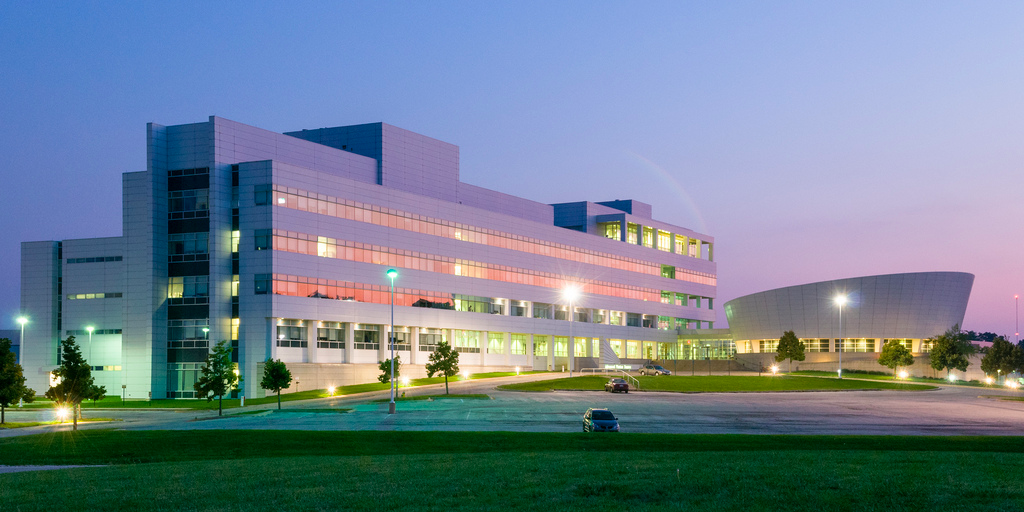
\includegraphics[height=5cm]{argonne.png}
	\end{center}
\end{wrapfigure}
\textbf{Argonne National Laboratory}\\
Located in Lemont, Illinois, Argonne works closely with universities, industry, and other national labs to help make an impact on the atomic, human, and global scale. With 14 research divisions, five national scientific user facilities, and hundreds of research partners, attendees of this tour will be exposed to the diverse areas of research in nuclear science. Argonne is two-and-a-half-hour drive away. Bus transportation will be provided. On the tour, students will be guided around the site’s scientific and engineering facilities.\\

\setlength\intextsep{0pt}
\begin{wrapfigure}{L}{0.45\textwidth}
	\begin{center}
		% \vspace{-\baselineskip}
		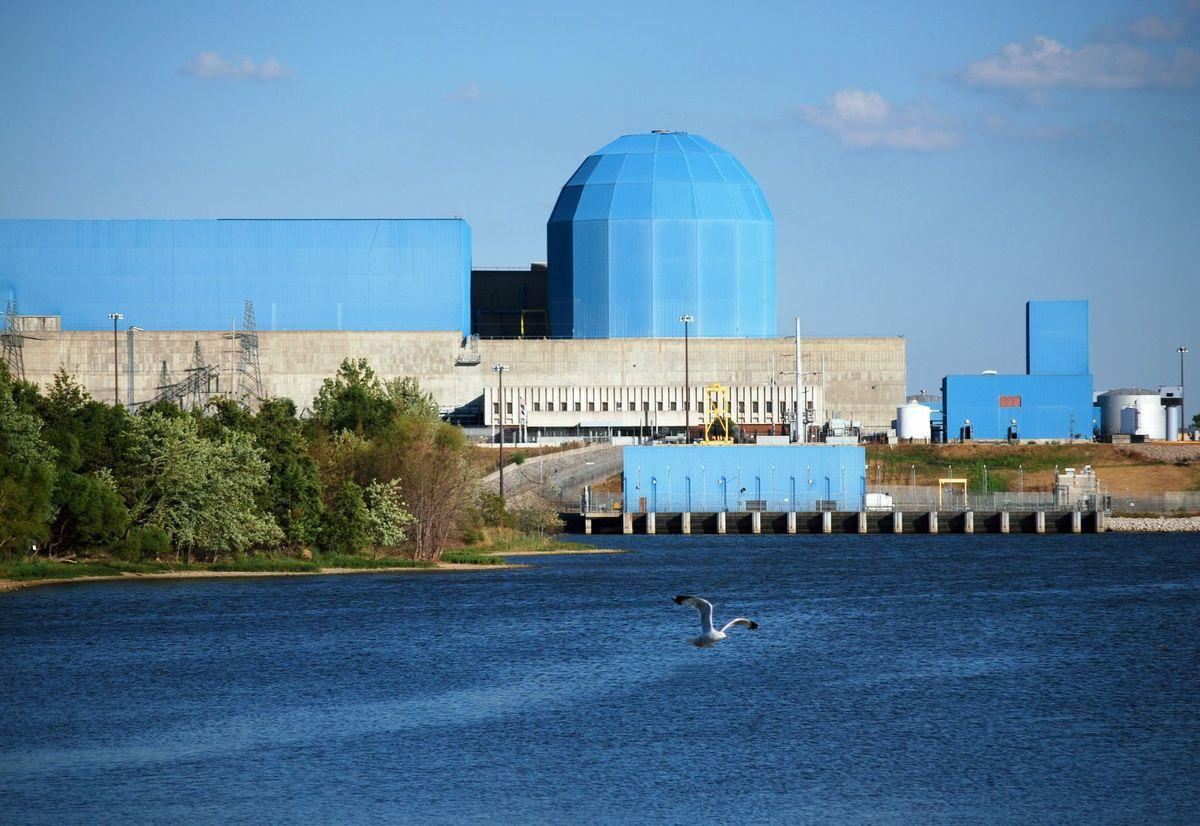
\includegraphics[height=5.5cm]{clintonpp.jpg}
	\end{center}
\end{wrapfigure}
\textbf{Clinton Power Station}\\
Located about 35 miles away from Champaign, the Clinton Power Station is an Exelon owned nuclear power plant that started operating at full power on September 15th, 1987. They currently serve over one million customers and operate 94.9$\%$ of the time. The tour will be held on Thursday morning and bus transportation will be provided. Attendees will be guided by a Clinton employee. The tour will include the control-room simulator that operator trainees use, and a chance to learn more about the site’s innovative safety, operation, and engineering practices.\\

\textbf{Starfire Industries LLC}\\
Starfire Industries is located at the south end of campus and works with federal organizations such as DARPA, Homeland Security, NASA, and others. They offer services in areas like neutron radiography, fabrication, and prototyping. Students will be able to get to the site by using the MTD busses that run continuously throughout the day and will be free to all conference attendees. Here, students will be able to learn more about Starfire products such as the IMPULSE pulsed power module, plasma sources, thin film systems, nGen neutron generators, neutron detectors, and the PICTORIS neutron radiography system. Starfire’s collaboration with government agencies and propensity for solving big problems related to plasma engineering make them a great place to learn about plasma processing applications.\\

\setlength\intextsep{0pt}
\begin{wrapfigure}{L}{0.48\textwidth}
	\begin{center}
		% \vspace{-\baselineskip}
		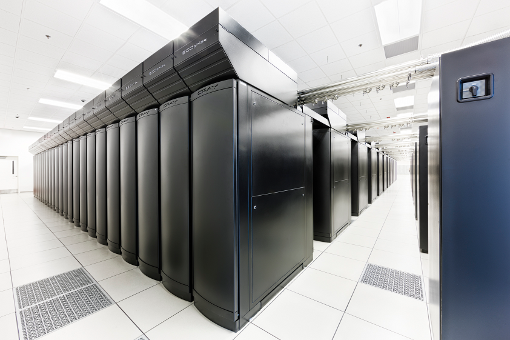
\includegraphics[height=5.5cm]{bw_front.png}
	\end{center}
\end{wrapfigure}
\textbf{National Center for Supercomputing Applications (NCSA)}\\
Also located on campus is NCSA, which houses Blue Waters, one of the most powerful supercomputers in the world. The NCSA is within walking distance from all conference hotels. During the tour, attendees will tour the machine room and witness some of the beautiful results it produces. Supercomputers like Blue Waters are important for solving computationally challenging problems and creating robust simulations for a variety of phenomena.\\

\subsubsection{Non-Technical Tours}



Brewery tours are staple social event and tour at the ANS Student Conference. Champaign-Urbana has several popular local breweries that give tours and tastings at their facilities. Due to this, we will be able to expand the number of attendees that can go on these tours over previous conferences. These will require sign up before the conference and we expect spots to fill up quickly.\\


\setlength\intextsep{0pt}
\begin{wrapfigure}{L}{0.3\textwidth}
	\begin{center}
		% \vspace{-\baselineskip}
		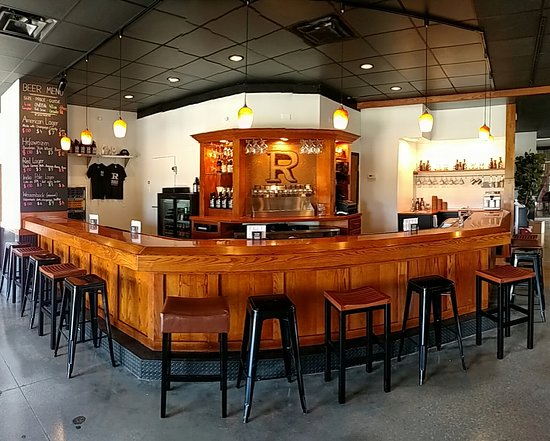
\includegraphics[width=0.28\textwidth]{riggs.jpg}
		\caption{Riggs Brewery}
	\end{center}
\end{wrapfigure}

\textbf{Riggs Brewery Tour}\\
For 21+ attendees, two tours of a local brewery will be included in our tours list Thursday afternoon from 3-5pm. Find out how Riggs makes their beer and taste test it along the way. Each tour will last approximately one hour and accommodates up to 20 people per tour. Riggs is located in east Urbana. Transportation to and from the brewery will be provided. \\ 
\setlength\intextsep{0pt}
\begin{wrapfigure}{R}{0.3\textwidth}
	\begin{center}
		% \vspace{-\baselineskip}
		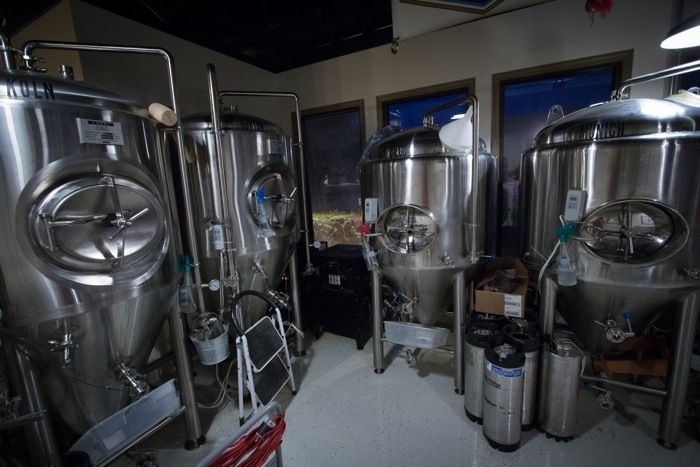
\includegraphics[width=0.28\textwidth]{triptych.jpeg}
		\caption{Triptych Brewery}
	\end{center}
\end{wrapfigure}
\newline
\vspace{1cm}
\newline


\textbf{Triptych Brewery Tour}\\
For 21+ attendees, Triptych offers two tours that run around 1.5 hours for roughly 30 people each that includes several beer tastings throughout. Tours will be from 2-5pm on Thursday afternoon. Triptych is located in Savoy, IL, just 15 minutes from campus. Transportation to and from the brewery will be provided.\\
% \newline
% \newline
\newline
\vspace{2cm}
\newline
% \newline
\textbf{University Tour}\\
Attendees will be able to take a tour of the UIUC campus. They will start at the Talbot Laboratory where the department of Nuclear Plasma and Radiological Engineering is located. Here, students will get to see the Virtual Education and Research Laboratory to see how virtual reality technology can be adapted and applied to educational methods. There are also many other historical artifacts on display for participants to see. Afterwards, students will be led to various noteworthy locations unique to UIUC.\\ 	


\subsection{Socials}

\subsubsection{Illini Union Rec Room Lockout}
The Illini Union Rec Room is located in the basement of the Union building. A Rec Room lockout gives ANS exclusive access to 14 bowling lanes, 12 billiard tables, and coin-operated arcade games following dinner at the Krannert Center for Performing Arts, only a short walk away through the University of Illinois main quad! This space can accompany up to 150 people, with extra tables outside of the Rec Room for socializing, playing board games, or having a late night snack or coffee with professionals or students from other universities.

% Illini Union Rec Room Picture
\begin{figure}[H]
	\centering
	\begin{subfigure}{0.5\textwidth}
		\centering
		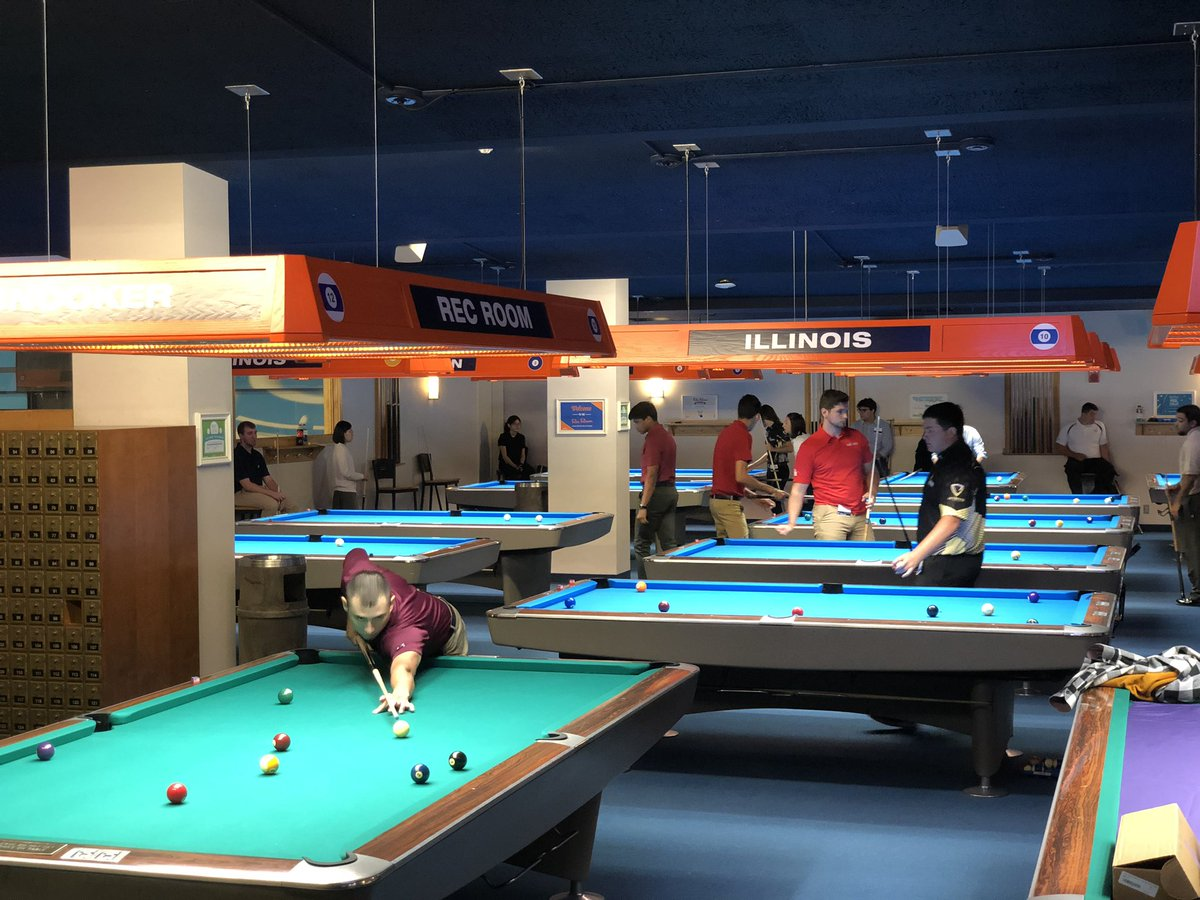
\includegraphics[width=0.9\linewidth]{union_recroom1.png}
	\end{subfigure}%
	\begin{subfigure}{0.5\textwidth}
		\centering
		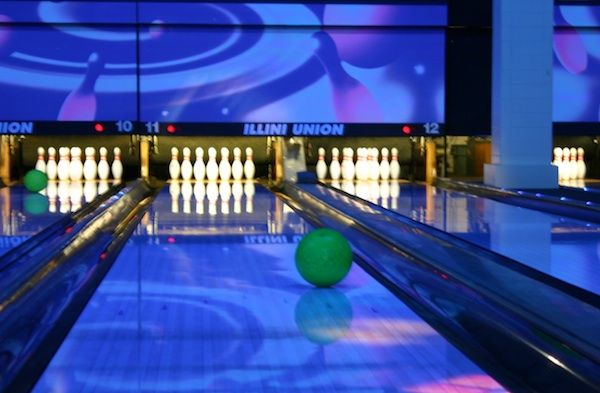
\includegraphics[width=0.9\linewidth]{union_recroom2.png}
	\end{subfigure}		
\end{figure} 

\subsubsection{77 Club at Memorial Stadium}
Memorial Stadium is not only home to the Fighting Illini football team, but also to exquisite event space overlooking Zuppke Field. The sixth level of Memorial Stadium is home of the magnificent 77 Club, which honors Illini great, the ``Galloping Ghost'' Red Grange. This 5,020 square foot space is located midfield and features an outdoor patio area overlooking the city of Champaign, for a combined total space of 9,740 square feet. This event will take place following dinner at I Hotel Conference Center, and is just a short and scenic walk away past the State Farm Center (formerly the historic Assembly Hall). Tables will be set up around a stage featuring live music and a dance floor and drinks will be served. This is the perfect event to incorporate a little bit of Illinois history with music, dancing, and socializing! 

% 77 Club Picture
\begin{figure}[H]
	\centering
	\begin{subfigure}{0.5\textwidth}
		\centering
		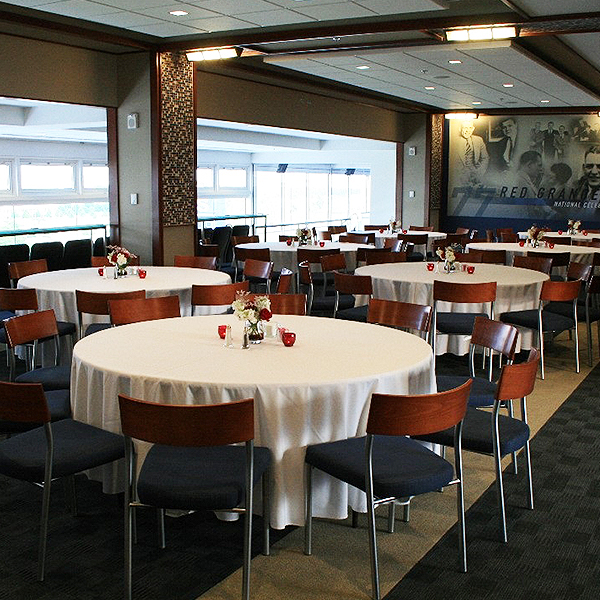
\includegraphics[width=0.7\linewidth]{77club1.png}
	\end{subfigure}%
	\begin{subfigure}{0.5\textwidth}
		\centering
		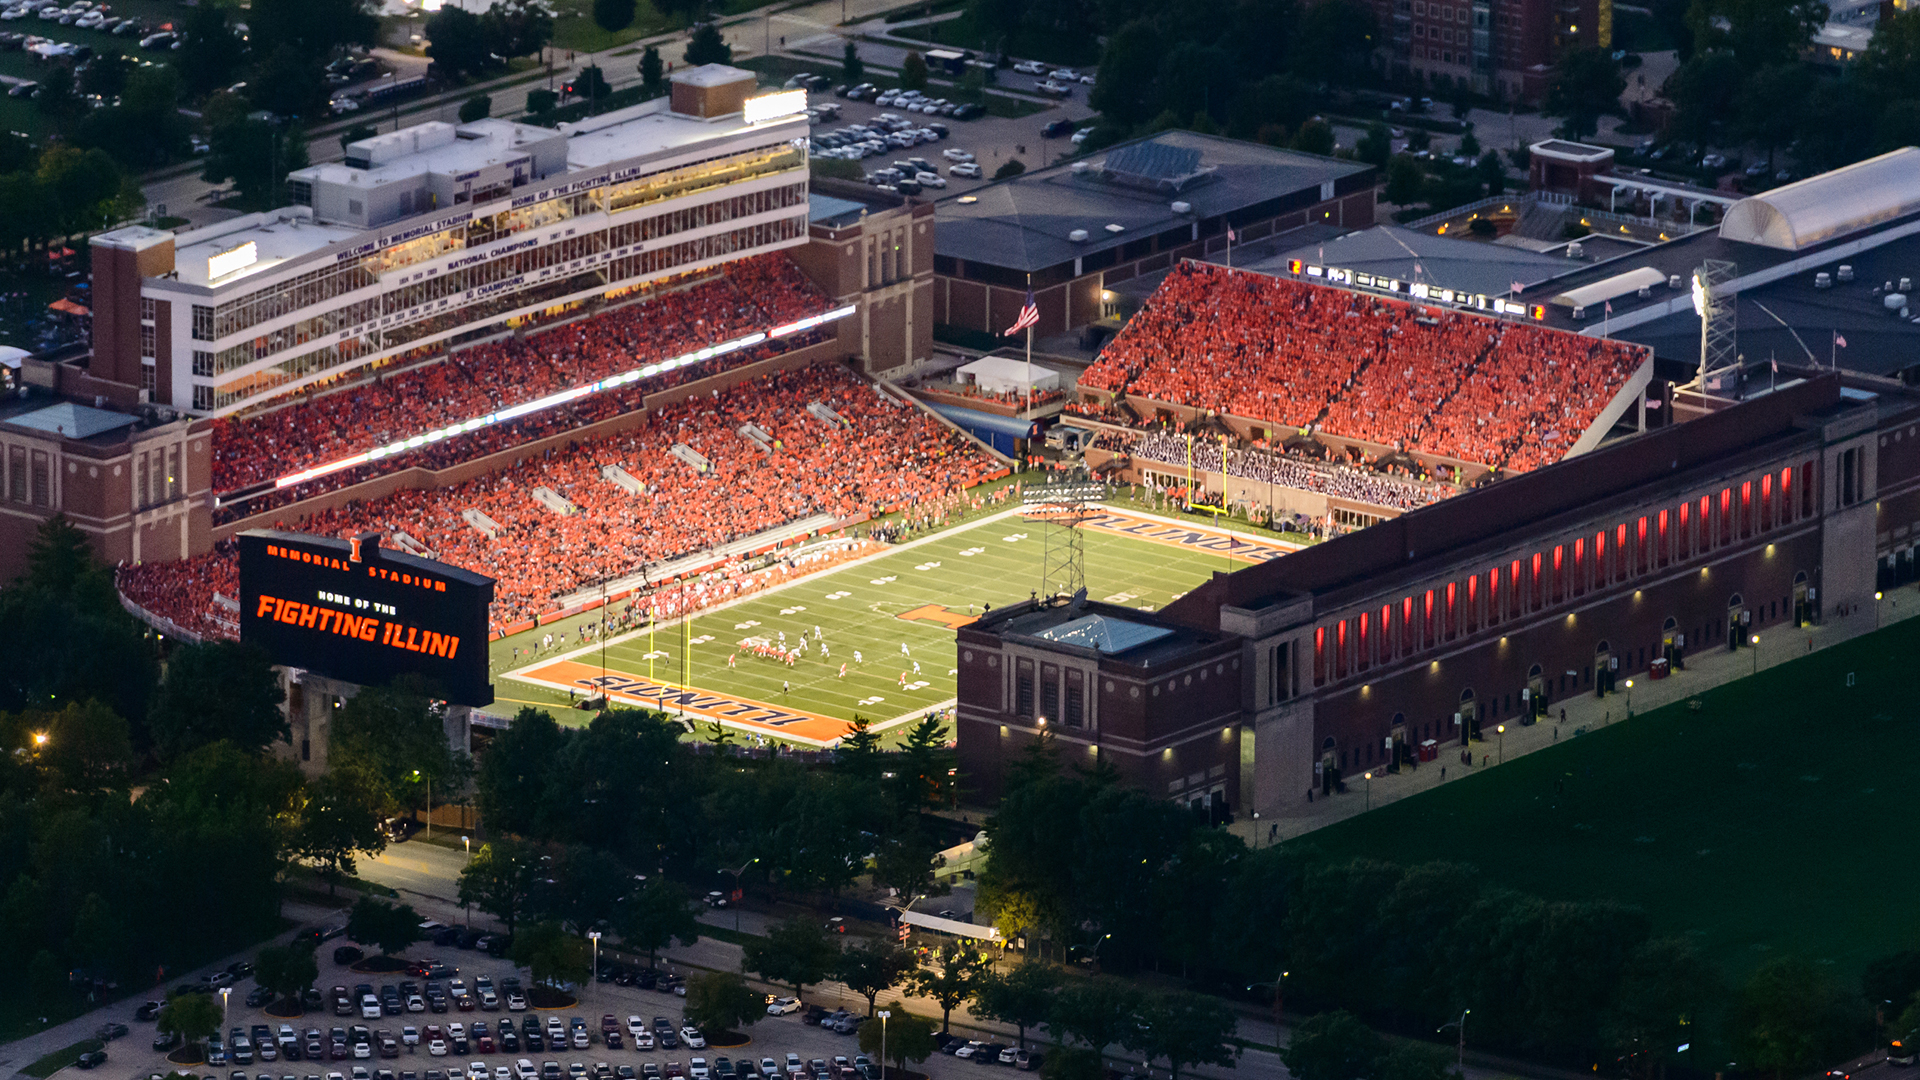
\includegraphics[width=0.9\linewidth]{77club2.png}
	\end{subfigure}		
\end{figure} 

\subsubsection{Pour Bros. Taproom in Downtown Champaign}
Welcome to Illinois' first pour-your-own taprooms. Pour Bros. Taproom is located in the heart of the historic downtown Champaign area and features 28 pour-your-own taps: beers, ciders, meads and wine\ldots all poured by you, one ounce at a time. Socialize over the vintage games Pour Bros has to offer: skeeball, bubble hockey, steel tip darts, DAGZ and more! If you are feeling more on the leisurely side, Pour Bros features live music in a spacious and comfortable seating area for you to get your networking on.

% Pour Bros Picture
\begin{figure}[H]
	\centering
	\begin{subfigure}{0.5\textwidth}
		\centering
		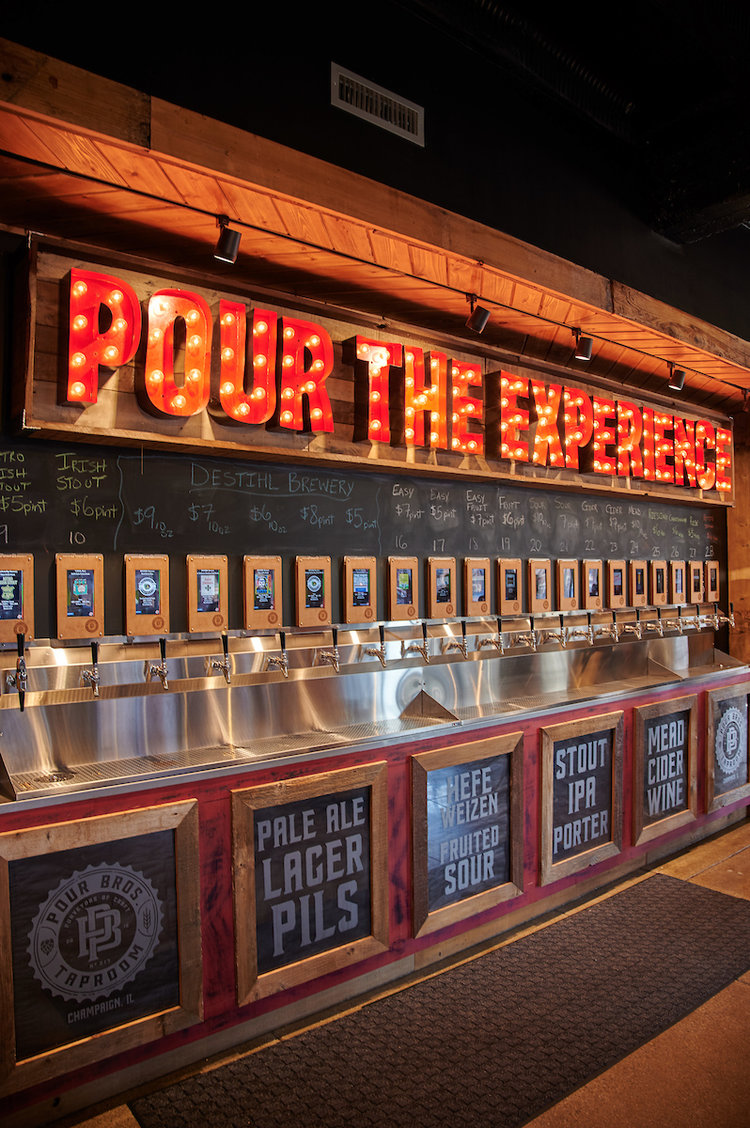
\includegraphics[width=0.5\linewidth]{pour_bros2.png}
	\end{subfigure}%
	\begin{subfigure}{0.5\textwidth}
		\centering
		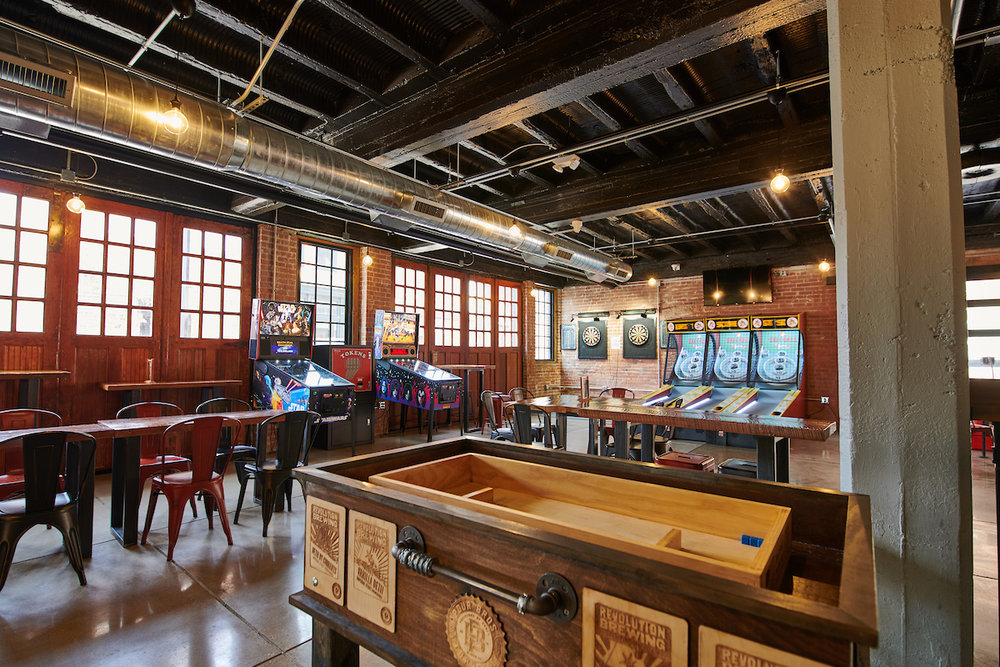
\includegraphics[width=0.9\linewidth]{pour_bros1.png}
	\end{subfigure}		
\end{figure} 

\subsubsection{Under 21 Social: University of Illinois Ice Arena}
For students under the drinking age that cannot attend the Pour Bros. Taproom social event, the University of Illinois Ice Arena is another option that is only a brief walking distance from the Union. It was built in 1931 and offers a unique option for skating get-togethers from broomball and hockey to group skating parties. The Ice Arena is a 55,000 square foot facility and is the only one in Champaign-Urbana. The dimensions of the rink are 192' by 115' with a 1,200 seat arena surrounding. There are four public locker rooms, four party areas, and two Zambonis in the facility. The Center Ice Cafe offers hot chocolate, coffee, smoothies, fountain drinks, and more to quench your thirst.  Snacks and concession items are also available.

% Ice Arena Picture
\begin{figure}[H]
	\centering
	\includegraphics[width=0.8\textwidth]{ice_arena.png}
\end{figure}


\newpage
\section{Conference Management}

The Conference Planning Committee is separated into three categories: Co-Chairs, Directors, Coordinators. The three co-chairs are responsible for setting up major milestones and ensuring that those milestones are met. Together they oversee all three subcommittees. They will serve as the primary contacts between subcommittee chairs and the faculty as well as professionals. The co-chairs have the final word on all conference decisions. They serve as the faces of the conference. In this proposal we have decided to add a novel Co-Chair position: Diversity Co-Chair. This addition reflects our goal of celebrating the people behind the science and make this conference experience accessible to as many people as possible. 
The Directors are in charge of specialized subcommittees and are responsible for making decisions in those areas. They must communicate with their subcommittees and with other directors to make sure there are no conflicting decisions. The coordinators work in an even more specialized area and help the directors by handling a single task.\\

% \vspace{1cm}

% ===============================================
% This is the hierarchy breakdown
% ===============================================
% \begin{center}
% 	\begin{tikzpicture}[
% 		chair/.style={rectangle, text centered, draw,fill=blue!20, execute at begin node={\begin{varwidth}{9em}},
%    		execute at end node={\end{varwidth}}},
%    		committee/.style={rectangle,draw,fill=green!40, text centered, execute at begin node={\begin{varwidth}{7em}},
%    		execute at end node={\end{varwidth}}},
%    		coordinator/.style={rectangle,draw,fill=red!30, text centered, execute at begin node={\begin{varwidth}{7em}},
%    		execute at end node={\end{varwidth}}},
% 		grandchild/.style={grow=down,xshift=1em,anchor=west,
% 		edge from parent path={(\tikzparentnode.south) |- (\tikzchildnode.west)}, execute at begin node={\begin{varwidth}{8em}},
%    		execute at end node={\end{varwidth}}},
% 		first/.style={level distance=12ex},
% 		second/.style={level distance=24ex},
% 		third/.style={level distance=36ex},
% 		level 1/.style={sibling distance=11em}]
% 	    % Parents
% 	    \coordinate
% 	      child[grow=left] {node[chair,anchor=east]{General Co-Chair \\ (Sam Dotson)}}
% 	      child[grow=right] {node[chair,anchor=west]{Technical Co-Chair\\ (Jeremy Mettler)}}
% 	      child[grow=down,level distance=3ex]
% 	    [edge from parent fork down]
% 	    % Children and grandchildren
% 	    child{node[committee] {Non-Technical Subcommittee}
% 	      child[grandchild,first] {node[chair]{Logistics Chair}}
% 	      child[grandchild,second] {node[coordinator]{Hotels and Transportation}}
% 	      child[grandchild,third] {node[coordinator] {Hospitality and Catering}}}
% 	    child {node[committee] {Communications Subcommittee}
% 	      child[grandchild, first] {node[chair] {Publications Chair}}
% 	      child[grandchild, second] {node[coordinator]{Media}}
% 	      child[grandchild, third] {node[coordinator] {Program}}}
% 	    child{node[committee] {Financial Subcommittee}
% 	      child[grandchild,first] {node[chair]{Financial Chair}}
% 	      child[grandchild,second] {node[coordinator]{Registration}}
% 	      child[grandchild,third] {node[coordinator]{Sponsorship}}}
% 	    child {node[committee]{Technical Subcommittee}
% 	      child[grandchild,first] {node[chair]{Sessions Chair}}
% 	      child[grandchild,second] {node[coordinator]{Workshops}}
% 	      child[grandchild,third] {node[coordinator]{Career Fair}}};
% 	\end{tikzpicture}
% \end{center}
\begin{center}
	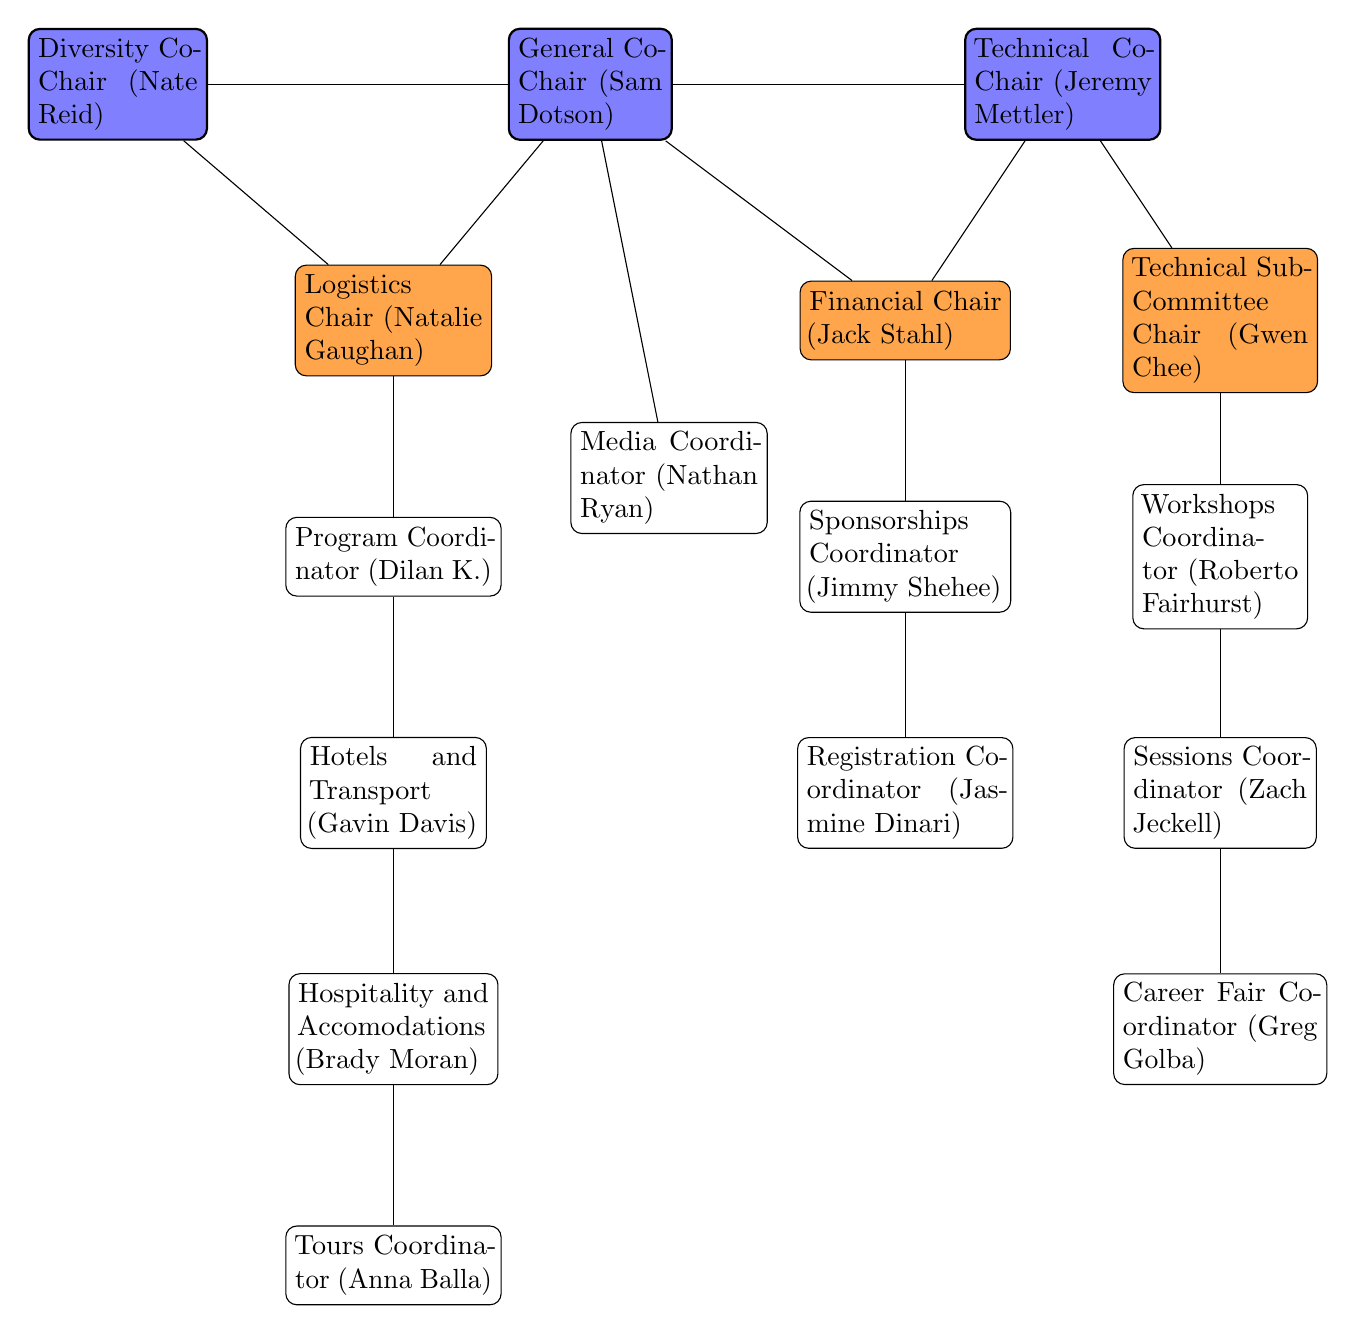
\begin{tikzpicture}
		\node (gen chair) [chair] {General Co-Chair (Sam Dotson)};
		\node (tech chair) [chair, right of = gen chair, xshift = 5cm] {Technical Co-Chair (Jeremy Mettler)};
		\node (div chair) [chair, left of = gen chair, xshift = -5cm] {Diversity Co-Chair (Nate Reid)};

		\node (log chair) [director, below of = gen chair, xshift = -2.5cm, yshift = -2cm] {Logistics Chair (Natalie Gaughan)};
		\node (med coord) [coordinator, below of = gen chair, xshift = 1cm, yshift = -4cm] {Media Coordinator (Nathan Ryan)};
		\node (prog coord) [coordinator, below of = log chair, yshift = -2cm] {Program Coordinator (Dilan K.)};
		\node (hat coord) [coordinator, below of = prog coord, yshift = -2cm] {Hotels and Transport (Gavin Davis)};
		\node (hoa coord) [coordinator, below of = hat coord, yshift = -2cm] {Hospitality and Accomodations (Brady Moran)};
		\node (tours coord) [coordinator, below of = hoa coord, yshift = -2cm] {Tours Coordinator (Anna Balla)};


		\node (tsc chair) [director, below of = tech chair, xshift = 2cm, yshift = -2cm] {Technical Sub-Committee Chair (Gwen Chee)};
		\node (work coord) [coordinator, below of = tsc chair, yshift = -2cm] {Workshops Coordinator (Roberto Fairhurst)};
		\node (sesh coord) [coordinator, below of = work coord, yshift = -2cm] {Sessions Coordinator (Zach Jeckell)};
		\node (cf coord) [coordinator, below of = sesh coord, yshift = -2cm] {Career Fair Coordinator (Greg Golba)};
		
		\node (fin chair) [director, below of = tech chair, xshift = -2cm, yshift = -2cm] {Financial Chair (Jack Stahl)};
		\node (spon coord) [coordinator, below of = fin chair, yshift = -2cm] {Sponsorships Coordinator (Jimmy Shehee)};
		\node (reg coord) [coordinator, below of = spon coord, yshift = -2cm] {Registration Coordinator (Jasmine Dinari)};

		\draw  (gen chair) -- (tech chair);
		\draw  (gen chair) -- (div chair);
		\draw  (gen chair) -- (log chair);
		\draw  (log chair) -- (prog coord);
		\draw  (prog coord) -- (hat coord);
		\draw  (hat coord) -- (hoa coord);
		\draw  (hoa coord) -- (tours coord);
		\draw  (gen chair) -- (med coord);
		\draw  (tech chair) -- (fin chair);
		\draw  (gen chair) -- (fin chair);
		\draw  (tech chair) -- (tsc chair);
		\draw  (fin chair) -- (spon coord);
		\draw  (spon coord) -- (reg coord);
		\draw  (tsc chair) -- (work coord);
		\draw  (work coord) -- (sesh coord);
		\draw  (sesh coord) -- (cf coord);
		\draw  (div chair) -- (log chair);

	\end{tikzpicture}
\end{center}

% ===============================================
% ===============================================
% ===============================================





\subsection{Position Responsibilities}

\begin{itemize}
	\item $\large\textbf{\textit{General Co-Chair}}$\\
	In addition to the responsibilities outlined above, the General Co-Chair oversees the
	Non-technical Subcommittee, the Media Coordinator, and the Financial Subcommittee. He works with the Technical Co-Chair in talking to sponsors, companies, and planning full committee meetings. 
	\item $\large\textbf{\textit{Technical Co-Chair}}$\\
	In addition to the responsibilities outlined above, the Technical Co-Chair primarily oversees the
	Technical Subcommittee. Works with the General Co-Chair to plan full committee meetings and completes any remaining tasks to ensure that milestones are met.
	\item $\large\textbf{\textit{Diversity Co-Chair}}$\\
	In addition to the responsibilities outlined above, the Diversity Co-Chair is responsible for making sure the conference is as inclusive, diverse, and accessible as possible. This includes: contacting minority serving institutions to encourage their students to attend the conference, ensuring socials and dinners are accessible, verifies that the final list of speakers has adequate representation, and more. We believe the example set by UIUC will make this role a staple of future conferences.

	\item $\textbf{Non-Technical Subcommittee}$\\
	The Non-Technical Subcommittee oversees, arranges, and executes all actions related to hospitality, transportation, special events, and non-technical workshops and panels. This committee keeps the theme of the conference in mind when organizing all events. They ensure that the conference runs smoothly.
	\begin{itemize}
		\item[$\circ$] $\textbf{Logistics Chair}$\\
		The Logistics Chair is in charge of planning all tours and non-technical workshops and panels. Organizes speakers during dinners. Recruits student volunteers to staff events and sessions during the conference.
		Also responsible for keeping track of the subcommittee and reporting to the Co-Chairs.
		\item[$\circ$] $\textbf{Hotels and Transportation Coordinator}$\\
		Coordinates with ANS National to negotiate room rates and room blocks for hotels. Reserves busses for the 
		necessary times and events. Works with the Hospitality and Catering Coordinator and the Logistics Chair.
		\item[$\circ$] $\textbf{Hospitality and Catering Coordinator}$\\
		Responsible for planning and organizing all catered meals for the conference. that includes contacting the catering services, reserving the venues where meals are held, and making sure the venues are staffed.
		\item[$\circ$]$\textbf{Tours Coordinator}$\\
		The tours coordinator organizes tours and works with the transportation coordinator to ensure that transportation is available during the conference for these tours.
		\item[$\circ$]$\textbf{Program Coordinator}$\\
		The program coordinator creates programs for the conference, sets the conference schedule to minimize overlap between events and increase student involvement. Communicates with other coordinators and subcommittees about the schedule of events. Designs and purchases T-shirts for attendees. Arranges gift bags for attendees. Works with sponsorship coordinator to create gift bags.
	\end{itemize}
	\item $\textbf{Financial Subcommittee}$\\
	The Financial Subcommittee oversees, arranges, and executes all actions related to banking, sponsorship, registration, reimbursement, budgeting, and monetary exchanges. This committee works closely with the General and Technical Co-Chairs.
	\begin{itemize}
		\item[$\circ$] $\textbf{Financial Chair}$\\
		Manages the ANS Planning Committee account with Busey Bank and ANS National. The account coordinator is also responsible for keeping track of receipts, setting a budget for the committee, keeps track of all transactions, 
		\item[$\circ$] $\textbf{Registration Coordinator }$
		Handles the registration for professional and student attendees. Communicates the number of attendees to the Program Coordinator. 
		\item[$\circ$] $\textbf{Sponsorship Coordinator}$\\
		Assists the Financial Co-Chair with matters involving sponsorship as well as working closely with the Registration and Account Coordinators and the General and Technical Co-Chairs. Works with the Program Coordinator on gift bag items and works with the Career Fair Coordinator.
	\end{itemize}
	\item $\textbf{Technical Subcommittee}$\\
	The Technical Subcommittee works with the Technical Co-Chair to process student abstracts and set up 
	technical workshops, panels and sessions. 
	\begin{itemize}
		\item[$\circ$] $\textbf{Technical Subcommittee Chair}$\\
		 Also responsible for ensuring that judges understand the judging criteria, and organizes the award ceremony.
		Keeps track of subcommittee progress and reports to the General and Technical Co-chairs.
		\item[$\circ$] $\textbf{Sessions Coordinator}$\\
		Responsible for organizing presentation, poster sessions, and technical
		panels. Makes sure that all rooms are properly set up with equipment to ensure smooth technical sessions.
		\item[$\circ$] $\textbf{Workshops Coordinator}$\\
		Organizes workshops locations, times, staffing, costs, supplies, student enrollment
		and any other tasks required to have successful workshops. Also assists the Sessions Chair when needed.
		\item[$\circ$] $\textbf{Career Fair Coordinator}$\\
		Oversees staffing and support for the career fair as well as working with the Sponsorship
		Coordinator to ensure a successful career fair. Also assists the Sessions Chair when needed.
	\end{itemize}
	\item $\textbf{Media Coordinator}$\\
		The Media Coordinator is reponsible for designing the conference website, constantly updating social media presence,
		and obtains information from other members of the planning committee for the website. 
\end{itemize}

\newpage
\subsection{Planning Committee Biographies}

\setlength\intextsep{0pt}
\begin{wrapfigure}{L}{0.35\textwidth}
	\begin{center}
		\vspace{-\baselineskip}
		\includegraphics[height=15\baselineskip]{dotsons2.jpg}
	\end{center}
\end{wrapfigure}
$\textbf{General Co-Chair - Sam Dotson}$\\
Sam graduated with a B.S. in Physics from UIUC in 2019. He attended his first ANS student conference in April 2019 and was so inspired by his experience that he decided to pursue graduate work in nuclear engineering rather than physics. Now he does research on machine learning applications and computational reactor physics with Dr. Kathryn Huff in the ARFC group. Hosting a student conference that will inspire others the way he was inspired is one of his top priorities this year. He has experience planning activities for student organizations such as Guidance for Physics Students (GPS) and has experience fundraising for the College of Lake County (CLC). He helped set a record amount of donations at the 2016 CLC Foundation Gala, where he was an invited speaker and volunteer. He will be attending the ANS National conference in November 2019, as well as the ANS Student Conference 2020 at North Carolina State University.\\

\setlength\intextsep{0pt}
\begin{wrapfigure}{R}{0.35\textwidth}
	\begin{center}
		\vspace{-\baselineskip}
		\includegraphics[height=15\baselineskip]{mettlerj.jpg}
	\end{center}
\end{wrapfigure}
$\textbf{Technical Co-Chair - Jeremy Mettler}$\\
Jeremy graduated with a B.S. in Nuclear, Plasma, and Radiological Engineering from UIUC in 2018, and is now attending as a 2nd-year graduate student studying plasma science under Dr. David Ruzic. He has been heavily involved in the UIUC student chapter of ANS since his freshman year, serving on the executive board for three years as External Vice President and President. Jeremy has attended the past five ANS Student Conferences, which serve as an inspiration for his involvement in this proposal process. He is dedicated to making sure that future generations of students are able to have the same amazing experiences through ANS as he had, especially at the ANS Student Conference. Outside of ANS, he has held a summer internship at Oak Ridge National Lab, and is currently focusing his research towards combined laser-plasma systems for materials processing.\\

\setlength\intextsep{0pt}
\begin{wrapfigure}{L}{0.35\textwidth}
	\begin{center}
		\vspace{-\baselineskip}
		\includegraphics[height=15\baselineskip]{ncreid2.jpg}
	\end{center}
\end{wrapfigure}
$\textbf{Diversity Co-Chair - Nathan Reid}$\\
Nate graduated with a B.S. in Nuclear, Plasma, and Radiological Engineering from UIUC in 2016. He is currently attending UIUC as a 4th-year Ph.D. student in the field of fusion and plasma science and engineering under the advisory of Prof. Jean Paul Allain. Nate is currently performing his thesis research at Oak Ridge National Laboratory, where he has spent the last three summers working on a multitude of projects in the nuclear structural materials group, with a focus on the technological assessment of plasma facing materials such as advanced tungsten alloys and composites under the mentorship of Dr. Lauren Garrison. The mechanisms of radiation-induced effects on tungsten are not well understood, and Nate's research provides the information necessary to prevent these effects from diminishing the ability of tungsten to shield the structural materials, pumping systems, and cooling pipes in future fusion reactors. These components are all vital to the success of fusion power generation. He believes that once we have a recipe for tungsten that is sustainable for a commercial fusion plant, fusion may be viable as an alternative energy source for our future's growing energy demands. 

Nate has attended four of the last five ANS Student Conferences and was a student paper competition finalist at the TOFE embedded topical of the 2018 ANS Winter Meeting, presenting his work on glow-discharge optical emission spectroscopy of tungsten neutron-transmutation elements. Nate is recognized by the ANS section at UIUC for his outstanding graduate service in the last year, and served as the Women in Nuclear UIUC chapter Vice President. He was part of the executive team that received the national student chapter excellence award at the 2019 Women in Nuclear national conference, of which he was awarded a student sponsorship to attend. Nate is ecstatic about working alongside his ANS student section as Diversity Co-Chair and setting goals to bring inclusion to the conference.\\

$\textbf{Financial Co-Chair}$\\
\setlength\intextsep{0pt}
\begin{wrapfigure}{R}{0.35\textwidth}
	\begin{center}
		\vspace{-\baselineskip}
		\includegraphics[scale=0.1]{stahlj.jpg}
	\end{center}
\end{wrapfigure}
$\textbf{Account Coordinator - Jack Stahl}$\\
\lipsum[1-1]

\setlength\intextsep{0pt}
\begin{wrapfigure}{L}{0.35\textwidth}
	\begin{center}
		\vspace{-\baselineskip}
		\includegraphics[height=15\baselineskip]{dinarij.jpg}
	\end{center}
\end{wrapfigure}
$\textbf{Registration Coordinator - Jasmine Dinari}$\\
Jasmine is a frehsman studying Nuclear, Plasma, and Radiological Engineering at UIUC, as well as minors in French and Physics. She is starting research with Dr. Andruczyk, who is currently at the head of the HIDRA project. Powering the world through nuclear is one of her main interests, and she later hopes to participate in nuclear fusion research. The ANS Student Conference is an  amazing opportunity to share her interests in nuclear science. She gained organizational and leadership experience through various extracurriculars in high school and currently serves as the Professional Development Chair for the UIUC student chapter of Women in Nuclear. She plans on attending the 2020 ANS Student Conference at NC State.



\setlength\intextsep{0pt}
\begin{wrapfigure}{R}{0.35\textwidth}
	\begin{center}
		\vspace{-\baselineskip}
		\includegraphics[height=15\baselineskip]{sheheej.jpg}
	\end{center}
\end{wrapfigure}
$\textbf{Sponsorship Coordinator - James Shehee}$\\
Jimmy is a junior undergraduate student in UIUC's Nuclear, Plasma, and Radiological Engineering department, with a concentration in power, safety, and the environment. Jimmy has been an active member of the University's ANS student chapter since his freshman year, has held the positions of Secretary and External Vice President, and was chosen to receive the chapter's Undergraduate Outstanding Service Award in the spring of 2019. Jimmy was first introduced to the nuclear industry through the Nuclear Science Merit Badge in Boy Scouts, and he is excited about any opportunity to create similar experiences for students and the public. Outside of ANS, Jimmy is also the President of the Illini Venturing Crew. In the summer of 2019, Jimmy interned at Exelon's Quad Cities Generating Station, and will be returning for another summer in 2020. He is excited to attend his first ANS Student Conference in March 2020 at North Carolina State University.

$\textbf{Technical Subcommittee}$\\
\setlength\intextsep{0pt}
\begin{wrapfigure}{L}{0.35\textwidth}
	\begin{center}
		\vspace{-\baselineskip}
		\includegraphics[height=15\baselineskip]{cheeg.jpg}
	\end{center}
\end{wrapfigure}
$\textbf{Technical Subcommittee Chair- Gwen Chee}$\\
Gwen is a third year graduate student studying fuel cycles for advanced reactor designs with Dr. Kathryn Huff in the ARFC group. Last summer she had an internship at Argonne National Laboratory where she worked on (...) .She also serves as the president of the UIUC chapter of Women In Nuclear (WiN). Under her leadership, WiN-UIUC was honored with the Best Student Chapter award at the WiN National Meeting in 2019. She has also been involved with ANS and attended the 2018 ANS Student Conference in Florida and will be attending the upcoming ANS Student Conference at NC State in 2020. 

\setlength\intextsep{0pt}
\begin{wrapfigure}{R}{0.35\textwidth}
	\begin{center}
		\vspace{-\baselineskip}
		\includegraphics[height=15\baselineskip]{fairhurstr.jpg}
	\end{center}
\end{wrapfigure}
$\textbf{Workshops Coordinator - Roberto Fairhurst}$\\
Roberto graduated with a B.S. in Nuclear Engineering from Instituto Balseiro (Argentina) April 2018. He is now a 2nd-year graduate student at UIUC. He does research on computational multi-physics solvers applied to advanced reactors as part of the Advanced Reactors and Fuel Cycle group under the supervision of Dr. Kathryn Huff. He got experience in the organization of conferences during the planning and development of a technical workshop (TWOFCS19) that took place at UIUC in June 2019. His motivation for hosting a student conference is his passion for Nuclear Energy and his desire to transmit this passion to other students. He believes hosting the student conference at UIUC will help the field grow and thrive. This is also an opportunity to meet other people working in the field, share life experiences, and develop a stronger network.


\setlength\intextsep{0pt}
\begin{wrapfigure}{R}{0.35\textwidth}
	\begin{center}
		\vspace{-\baselineskip}
		\includegraphics[height=15\baselineskip]{jeckellz.png}
	\end{center}
\end{wrapfigure}
$\textbf{Sessions Coordinator - Zachary Jeckell}$\\
Zachary graduated with a B.S. in Nuclear, Plasma, and Radiological Engineering from UIUC in 2018 and is now a second year graduate student studying plasma engineering under Dr. David Ruzic. He has presented his research at two previous student conferences  and realized that he wanted to help bring this prestigious event to the University of Illinois. He strongly believes that the group of students at UIUC are capable of such a feat and that the University would make an excellent location for the conference because of its stellar program and wonderful faculty. He plans to attend the next ANS student conference at NC State to present research on chemical vapor deposition using atmospheric pressure plasma. 
\clearpage
\setlength\intextsep{0pt}
\begin{wrapfigure}{R}{0.35\textwidth}
	\begin{center}
		\vspace{-\baselineskip}
		\includegraphics[height=15\baselineskip]{golbag.jpg}
	\end{center}
\end{wrapfigure}
$\textbf{Career Fair Coordinator - Grzegorz Golba}$\\
Grzegorz Golba is a sophomore pursuing a B.S. in Nuclear Engineering with a physics minor in the plasma and fusion science concentration. He is now studying material interactions with plasma under Dr. Daniel Andruczyk. Grzegorz attended the 2019 ANS Student Conference in Virginia, reaffirmed his desire to study of nuclear science. He seeks new opportunities to engage with the nuclear science community and is excited for the possibilities of hosting a student conference at UIUC. 
\newline
\vspace{3cm}
\newline
$\textbf{Non-Technical Subcommittee}$
\setlength\intextsep{0pt}
\begin{wrapfigure}{R}{0.35\textwidth}
	\begin{center}
		\vspace{-\baselineskip}
		\includegraphics[height=15\baselineskip]{gaughann.JPG}
	\end{center}
\end{wrapfigure}

$\textbf{Logistics Chair - Natalie Gaughan}$\\
Natalie earned her B.S. in Nuclear Engineering from the University of Wisconsin-Madison in 2017. She has completed two summer internships at Argonne National Laboratory where she worked with various neutronics codes. Natalie then spent a year in Vienna as an intern at the International Atomic Energy Agency, where she helped organize and evaluate nuclear data for medical isotope production. She is now a graduate student at UIUC intending to research radiological science and nuclear medicine. As an undergraduate, Natalie attended two ANS student conferences which played a huge role in obtaining internships and inspired her decision to attend graduate school. Natalie knows firsthand how the ANS student conferences can be influential in students’ education and career development, and would love to help younger students experience the same benefits. She will also be attending the upcoming ANS student conference in 2020 at NC State.

\setlength\intextsep{0pt}
\begin{wrapfigure}{L}{0.35\textwidth}
	\begin{center}
		\vspace{-\baselineskip}
		\includegraphics[height=15\baselineskip]{kdilan.jpg}
	\end{center}
\end{wrapfigure}
$\textbf{Program Coordinator - Dilan Kurukulasuriya}$\\
Dilan Kurukulasuriay is a sophomore pursuing a B.S. in Nuclear, Plasma, and Radiological Engineering, along with a minor in Physics and Mathematics. He has been active in ANS at UIUC since the start of his freshman year, and he currently serves as the Outreach Chair on the Executive Board. Dilan has worked at the Center for Plasma-Material Interactions lab since the start of his freshman year on HIDRA, and he stayed on campus over the summer to continue to do so. Dilan attended the 2019 ANS Student Conference and it was the highlight of his freshman year of college. He is interested in fusion science research, specifically the materials interaction aspect. He also plans on attending the upcoming student conference at NC State in 2020.


\setlength\intextsep{0pt}
\begin{wrapfigure}{L}{0.35\textwidth}
	\begin{center}
		\vspace{-\baselineskip}
		\includegraphics[height=15\baselineskip]{davisg.jpg}
	\end{center}
\end{wrapfigure}
$\textbf{Hotels and Transportation Coordinator - Gavin Davis}$\\
Gavin is currently pursuing a B.S. in Nuclear, Plasma, and Radiological Engineering from UIUC and plans to graduate in 2022. He has been involved with the ANS-UIUC since his freshman year and has dedicated his time to outreach events and increasing public awareness of nuclear science and nuclear energy. He has accomplished this through events such as UIUC's Engineering Open House. It was an event he enjoyed as a kid and hopes to help other children develop an interest in nuclear sciences. He also returns to his high school to talk about his experience at UIUC. He looks forward to learning more about nuclear fission technology and to make advancements in nuclear science and in the nuclear energy sector as a whole. He looks forward to attending the student conference at NC State in 2020.

\setlength\intextsep{0pt}
\begin{wrapfigure}{R}{0.35\textwidth}
	\begin{center}
		\vspace{-\baselineskip}
		\includegraphics[height=15\baselineskip]{moranb.jpg}
	\end{center}
\end{wrapfigure}
$\textbf{Hospitality and Catering Coordinator - Brady Moran}$\\
Brady a freshman in the Nuclear, Plasma, and Radiological Engineering program in the Plasma concentration. He is looking forward to putting his time and efforts toward ANS events throughout his years at UIUC. Last year, Brady planned a large tasting event, the Taste of Sauk Valley, which boasted 550 attendees, $\$$15,000 in revenue, and required him to coordinate 12 restaurants and various subcommittees. He is confident that this experience will help him make the Student Conference a great success. He will be attending the 2020 conference at NC State.




\setlength\intextsep{0pt}
\begin{wrapfigure}{L}{0.35\textwidth}
	\begin{center}
		\vspace{-\baselineskip}
		\includegraphics[height=15\baselineskip]{ballaa.jpg}
	\end{center}
\end{wrapfigure}
$\textbf{Tours Coordinator - Anna Balla}$\\
Anna is a junior in NPRE with a planned concentration in the power, safety, and the environment. She became interested in nuclear engineering after taking a general education class with an NPRE professor and learning about how effective nuclear power is at reducing carbon emissions. Anna is a teaching assistant for two classes in the NPRE department and is also very involved with the Women in Nuclear chapter at Illinois. In her spare time, she enjoys going to concerts, playing volleyball, and wishing she knew how to juggle.

\setlength\intextsep{0pt}
\begin{wrapfigure}{R}{0.35\textwidth}
	\begin{center}
		\vspace{-\baselineskip}
		\includegraphics[width=0.3\textwidth]{ryann.jpg}
	\end{center}
\end{wrapfigure}
$\textbf{Media Coordinator - Nathan Ryan}$\\
Nathan is pursuing a B.S. in Physics from UIUC. He graduated in the top five of his high school class, while holding down a part time managerial position and running a research project at Argonne National Laboratory concurrent with his Sophomore through Senior years of Secondary Education. His first experience with Nuclear Physics was at the National Superconducting Cyclotron Laboratory where he worked with grad students on rare Cadmium isotopes. He has experience with building appealing website pages, as well as social media communications. He believes that an online presence for this event will supplement the success of an already great set of programs and individuals involved. He is excited to attend the upcoming ANS Student Conference at NC State in 2020.


\subsection{Conflict Resolution}

Committee members should hold professionalism at the forefront of their composure in order to avoid and resolve issues amicably without the involvement of higher powers. As such, members are encouraged to settle conflicts without invoking this protocol. If an issue arises that immediately presents itself as overwhelming, the scope of the issue exceeds an individual’s ability to handle it, or the issue imposes certain implications that jeopardizes the mission of the planning committee, members should not hesitate to refer to this section. In the event of a conflict between members of the planning committee, a document for decision-making and
conflict resolution has been drafted and approved by the general committee. All General Committee members
are expected to abide by the resolution. Key points of the resolution are as follows:
\begin{enumerate}
	\item Subcommittees are encouraged to resolve conflicts internally and as democratically as possible. If an independent resolution cannot be reached, the Co-Chairs should be involved. The Co-Chairs have the final word on all decisions. If the Co-Chairs are unable to agree on a solution, the faculty advisor will be involved.
	\item Conflicts between individual committee members are to be resolved outside of the committee. Should such a conflict jeopradize the mission of the conference the Co-Chairs will be involved. 
	\item Any cases of misconduct or negligence will be handled appropriately by the Co-Chairs.
	\item For extreme cases of misconduct or negligence, separate steps for the removal and replacement of a
	member are outlined for general members, Subcommittee Chairs, and Co-Chairs. These include
	a discussion with the offending member, consultation of the Faculty Advisor, and a hearing with the
	General Committee to decide if removal is necessary.
\end{enumerate}

\subsection{Staffing Requirements}
Staffing for room breakdowns and setups, registration, socials, workshops, tours, etc.  will be supplied by either UIUC ANS members or students of the NPRE department. While it is likely that members of our student chapter will voluntarily fill all the staffing requirements of conference hosted events. If not, we will rely on other student organizations for support including, but not limited to: ACDIS and WIE. Participating in conference events on a staff level is a beneficial experience for any undergraduate who wants to become more familiar with ANS or support their ANS Chapter. Throughout the conference, interacting with registering students, driving groups to tour a scientific facility, and turning rooms for technical sessions provide plentiful opportunities for volunteers to interact with myriad members on a number of levels. Thus, it will be an overall positive experience for the volunteers. Quantitative needs are outlined in Appendix G.

% ===============================================
% Milestones
% ===============================================
\subsection{Milestones}

\begin{center}
\begin{longtable}{c |  c  c}
\hline\hline
Deadline & Task & Responsibility\\
\hline\hline

&November&\\
\hline\hline
& Announcement of 2021 Conference & \\
& Update milestones with lessons learned &\\
& Notify department of selection & Co-Chairs\\
& Confirm Conference Committee & Co-Chairs\\
& Finalize Conference Date & Co-Chairs\\
& Confirm Conference Reservations & Non-Technical\\
& Contact ANS National for support with hotel negotiations& Co-Chairs and Non-Technical\\
& Set up banking through Busey Bank and ANS National& Financial\\
\hline\hline
&December&\\
\hline\hline
&Finalize Facilities Reservations& Non-Technical\\
&Finalize Logo Design& Communications\\
&Begin Designing Website and Social Media& Communications\\
\hline\hline
&$\textbf{2020}$&\\
\hline\hline
&January&\\
\hline\hline
& Finalize meeting schedule& Co-Chairs\\
&&\\
\hline\hline
&February&\\
\hline\hline
& Launch social media plan& Communications\\
& Finalize list of potential speakers& Non-Technical\\
& Finalize technical topics& Technical\\
\hline\hline
&March&\\
\hline\hline
& Contact Speakers and Presenters& Non-Technical and Technical\\
\hline\hline
&April&\\
\hline\hline
& Attend Student Conference at NC State& All\\
& Request lessons learned from NC State& Co-Chairs\\
& Create sponsor letters and contact & General Co-Chair\\
& Prepare tour opportunities& Non-Technical\\
\hline\hline
&May&\\
\hline\hline
& Confirm tours and costs& Non-Technical\\
& Submit Progress Report to SSC& \\
& Create a Call for Papers & Technical and Communications\\
\hline\hline
&June&\\
\hline\hline
& Send Delegates to National Conference& Co-Chairs, All\\
\hline\hline
&July&\\
\hline\hline
& Confirm with all speakers and presenters& \\
& Report on sponsorship& Financial\\
& Reassess budget& Financial\\
\hline\hline
&August&\\
\hline\hline
& Update with sponsors& Financial\\
& Submit second progress to SSC& Co-Chairs\\
\hline\hline
&September&\\
\hline\hline
& Updates on conference deadlines& Financial\\
& Order gift bags& Non-Technical\\
\hline\hline
&October&\\
\hline\hline
& Confirm hotel blocks and contracts& Non-Technical\\
& Registration Opens& Financial\\
& Create and test online paper submission& Technical\\
\hline\hline
&November&\\
\hline\hline
& Attend Winter Conference 2020& Co-Chairs, All\\
& Finalize marketing material& Communications\\
& Report from winter conference & Co-Chairs\\
\hline\hline
&December&\\
\hline\hline
& Update website & Communications \\
& Third progress report to SSC& Co-Chairs\\
& Send out call for papers& Communications\\
\hline\hline
&$\textbf{2021}$&\\
\hline\hline
&January&\\
\hline\hline
& Confirm all judges, panelists, and speakers& Technical\\
& First paper deadline -- send to reviewers & Technical\\
& Recruit student volunteers& All\\
& Finalize tours& Non-Technical\\
& Finalize conference transportation& Non-Technical\\
\hline\hline
&February&\\
\hline\hline
& Finalize program& Communications\\
& Order gift bag items & Financial and Non-Technical\\
& Final Paper Deadline& Technical\\
& Finalize App& Communications\\
& Finalize budget& Financial\\
& Extended Paper Deadline& \\
\hline\hline
&March&\\
\hline\hline
& Print Programs& Communications\\
& Finalize Awards& Technical\\
& Finalize Staff Schedule& Non-Technical\\
& Prepare gift bags, print tags, and banners& Non-Technical\\
& Final progress report to SSC& Co-Chairs\\
\hline\hline
&April&\\
\hline\hline
& Host ANS Student Conference 2021 & \\
& Return seed money& Financial\\
& Process Student Reimbursements& Financial\\
& Finalize financial report& Financial\\
& Submit conference report& Co-Chairs\\
\hline\hline
\end{longtable}
\end{center}
\newpage
\section{Website and Social Media}
\subsection{Website}
Shortly after the host is announced, ANS-UIUC will purchase a domain name and create a website in conjunction with ANS National. The website will be hosted using GitHub pages, a free hosting service for static websites. Since there is no cost, the website can be hosted indefinitely. This webhost was selected because several members of the chapter possess knowledge and experience in using it for serving collaborative, Jekyll-based, and static HTML websites. The domain name can be purchased for as little as one dollar for the first year, and a little less than $\$20$ to maintain annually. If we need to cut costs or decide that a domain name ending in ".github.io" is fine we can drop the purchased domain name. The website will include important dates, costs, calendars, schedules, maps, emergency contact information, as well as a direct link to the paper submission site for the conference. The mobile web app will store downloaded maps, emergency contact information, and calendars for offline use while providing access to all features of the website as well.

\subsection{Social Media} 

\newpage
\section{Budget}



% =======================================================================================
% =======================================================================================
% =======================================================================================
% =======================================================================================
% Revenue Section
% =======================================================================================
% =======================================================================================
% =======================================================================================
% =======================================================================================

\subsection{Revenue}
We have compared the predicted and actual revenues from previous reports and used these to estimate our expected revenue. To maintain reasonable accuracy in the budget, we were financially conservative in our estimates to account for fluctuating economy and attendance numbers. Should our bid be selected, these conservative estimates will result in a smoother planning and execution process. We have also accounted an estimated number of waived professional registration based on previous conferences. This  correlates to the number of waived fees given in our expected tier sponsorship figures and also factors in discounts to speakers, panelists, and workshop instructors. \\

\begin{table}[H]
\centering
\caption*{\textbf{Attendance}}
\begin{tabular}{|c|c|c|c|}
\hline
    \textbf{Item} & \textbf{Quantity} & \textbf{Cost} & \textbf{Subtotal}	\\ 
\hline
	Student			&	443	&	\$40	&	\$17,720						\\
	Professional	&	127	& 	\$250	&	\$31,750						\\
	Waived			&	60	& 	-\$250	&	-\$15,000						\\
\hline
	\multicolumn{3}{|r|}{\textbf{Attendance Total:}}	&	\$34,470		\\
\hline
\end{tabular}
\end{table}

\vspace{10mm}

\begin{table}[H]
\centering
\caption*{\textbf{Sponsors}}
\begin{tabular}{|c|c|c|c|}
\hline
    \textbf{Package} & \textbf{Quantity} & \textbf{Cost} & \textbf{Subtotal}	\\ 
\hline
	World Savior	&	1	&	\$30,000	&	\$30,000						\\
	National Hero	&	3	& 	\$15,000	&	\$45,000						\\
	Local Prodigy	&	5	& 	\$10,000	&	\$50,000						\\
	Lifesaver		&	6	& 	\$5,000		&	\$30,000						\\
	Exhibitor+		&	3	& 	\$3,500		&	\$10,500						\\
	Exhibitor		&	5	& 	\$2,500		&	\$12,500						\\
	Good Samaritan	&	10	& 	\$1,500		&	\$15,000						\\
	Contributor		&	8	& 	\$1,000		&	\$8,000							\\
\hline
	\multicolumn{3}{|r|}{\textbf{Sponsors Total:}}	&	\$201,000				\\
\hline
\end{tabular}
\end{table}

\vspace{10mm}

\begin{table}[H]
\centering
\begin{tabular}{|c|}
\hline
    \textbf{Total Revenue: \$235,470}\\ 
\hline
\end{tabular}
\end{table}

% =======================================================================================
% =======================================================================================
% =======================================================================================
% =======================================================================================
% Expenses Section
% =======================================================================================
% =======================================================================================
% =======================================================================================
% =======================================================================================

\subsection{Expenses}
A conservative breakdown of conference expenses is outlined in Table \ref{table:budget} on page \pageref{table:budget}. All rooms hosted in the Union are provided to registered student organizations (such as ANS-UIUC) free of charge. This allows us to save significantly on event space. Meals catered through the University catering service reflect a 6.25\% sales tax in the total cost which is not represented in the unit cost. Gratuity is neglected because it is forbidden under the catering service’s policies, allowing us to save 20\% gratuity on meals. 
Under our most conservative estimates for budget and revenue, the spending margin is found to be 4.13\%. While this margin is tight, we feel this is justified as several costs in the expenses, such as reimbursements, are left significantly inflated as compared with previous years. Adopting previous years’ estimates of \$60,000 for travel reimbursements leaves a spending margin of 21.6\%, matching that of the most austere contingency plans provided in previous years. 
Assuming maximum expenses and an attendance of 450 students, the total cost per student is estimated at \$501.63. This number also includes the travel reimbursement, which was intentionally set to be considerably more generous than previous years to make the budget more conservative. Neglecting the cost of travel reimbursements, the average cost per student falls to \$276.63, at or below that estimated for previous years. In Appendix \ref{appendix:quotes} on page \pageref{appendix:quotes} there are quotes from Peria Charter and the Union to give some sense of costs.

% \hspace{-1.1cm}
\begin{table}[H]
    \caption{Budget Expenses}
    \label{table:budget}
    \makebox[\linewidth]{
        \begin{tabular}{|clcrccccr|}
    
        \hline
         & \multicolumn{1}{c}{\textbf{Item}} & \multicolumn{1}{c}{\textbf{Priority}} & \multicolumn{1}{c}{\textbf{Cost Per Unit}} & \multicolumn{1}{c}{\textbf{Thursday}} & \multicolumn{1}{c}{\textbf{Friday}} & \multicolumn{1}{c}{\textbf{Saturday}} & \multicolumn{1}{c}{\textbf{General}} & \multicolumn{1}{c}{\textbf{Total Cost}}\\     \hline\hline
         \multirow{10}{*}{\STAB{\rotatebox[origin=c]{90}{\textbf{Facilities}}}}
         & Technical Session AV      & I                         & $\$$ 13.80                & 1                         & 6                        & 6                         & -                         & $\$$179.40               \\
         & Technical Session Rooms   & I                         & $\$$ 0.00                 & -                         &  -                       &  -                        &  1                        & $\$$0.00                 \\
         & Panel AV                  & I                         & $\$$ 17.80                & -                         &   2                      &   2                       &   -                       & $\$$71.20                \\ 
         & Panel Rooms               & I                         & $\$$ 0.00                 & -                         &    -                     &    -                      &    1                      & $\$$0.00                 \\
         & Workshop AV               & I                         & $\$$ 17.80                & 2                         &     -                    &     -                     &     -                     & $\$$35.60                \\
         & Workshop Rooms            & I                         & $\$$ 0.00                 &  -                        &      -                   &      -                    &      1                    & $\$$0.00                 \\ 
         & Dinner Room (Ihotel)      & I                         & $\$$ 4,000.00             &   -                       &       -                  &       1                   &       -                   & $\$$4,000.00             \\
         & Dinner AV (Ihotel)        & I                         & $\$$ 0.00                 &    -                      &        -                 &        1                  &        -                  & $\$$0.00                 \\
         & Dinner Room (Garden Hotel)& I                         & $\$$ 4,000.00             &     1                     &         1                &         -                 &         -                 & $\$$8,000.00             \\ 
         & Dinner AV (Garden Hotel)  & I                         & $\$$ 0.00                 &      1                    &          1               &          -                &          -                & $\$$0.00                 \\ \hline
         &                           &                           &                           &                           &\multicolumn{3}{r}{Facilities Subtotal:}     & $\$$12,286.20            \\ \hline\hline
         \multirow{5}{*}{\STAB{\rotatebox[origin=c]{90}{\textbf{Transport}}}}
         & Shuttles From Hotel       & I                         & $\$$ 1,000.00             & 4                         & 4                        & 4                         & -                         & $\$$12,000.00            \\
         & Ihotel Dinner             & I                         & $\$$ 875.00               & -                         &  -                       &  4                        &  -                        & $\$$3,500.00             \\
         & Brewery/Starfire Tours    & II                        & $\$$ 875.00               & 1                         &   -                      &   -                       &   -                       & $\$$875.00               \\ 
         & Clinton Tour              & II                        & $\$$ 875.00               & 1                         &    -                     &    -                      &    -                      & $\$$875.00               \\
         & Argonne Tour              & II                        & $\$$ 875.00               & 1                         &     -                    &     -                     &     -                     & $\$$875.00               \\ \hline
         &                           &                           &                           &                           &\multicolumn{3}{r}{Transport Subtotal:}      & $\$$18,125.00            \\ \hline\hline
         \multirow{5}{*}{\STAB{\rotatebox[origin=c]{90}{\textbf{Food}}}}
         & Coffee/Tea                & III                       & $\$$ 1.95                 & -                         & 600                      & 600                       & -                         & $\$$2,486.25             \\
         & Garden Hotel Dinners*     & II                        & $\$$ 36.50                & 600                       & 600                      &  -                        &  -                        & $\$$46,537.50            \\
         & Ihotel Dinner             & II                        & $\$$ 27.50                & -                         &   -                      &   600                     &   -                       & $\$$17,531.25            \\ 
         & Dinner Cash Bars          & III                       & $\$$ 336.00               & 1                         &    1                     &    1                      &    -                      & $\$$1,071.00             \\
         & SSC Lunches               & II                        & $\$$ 16.50                & -                         &     -                    &     150                   &     -                     & $\$$2,629.69             \\ \hline
         &                           &                           &                           &                           &\multicolumn{3}{r}{Food Subtotal:}           & $\$$70,255.69            \\ \hline\hline
         \multirow{5}{*}{\STAB{\rotatebox[origin=c]{90}{\textbf{Socials}}}}
         & Ice Skating               & III                       & $\$$ 240.00               & 2                         & -                        & -                         & -                         & $\$$480.00               \\
         & Illini Rec Room           & III                       & $\$$ 490.00               &  -                        & 2                        &  -                        &  -                        & $\$$982.00               \\
         & Memorial Stadium Club 77  & III                       & $\$$ 2,000.00             & -                         &   -                      &   1                       &   -                       & $\$$2,000.00             \\ 
         & Club 77 Tab               & IV                        & $\$$ 3,000.00             & -                         &    -                     &    1                      &    -                      & $\$$3,000.00             \\
         & Guido's Tab               & IV                        & $\$$ 3,000.00             & -                         &     1                    &     -                     &     -                     & $\$$3,000.00             \\ \hline
         &                           &                           &                           &                           &\multicolumn{3}{r}{Socials Subtotal:}        & $\$$9,462.00             \\ \hline\hline
         \multirow{7}{*}{\STAB{\rotatebox[origin=c]{90}{\textbf{Miscellaneous}}}}
         & Conference Programs       & I                         & $\$$ 2,133.90             & -                         & -                        & -                         & 1                         & $\$$2,133.90             \\
         & Lanyards                  & I                         & $\$$ 2.54                 &  -                        & -                        &  -                        &  600                      & $\$$1,524.00             \\
         & Award Certificates        & III                       & $\$$ 2.50                 & -                         &   -                      &   50                      &   -                       & $\$$125.00               \\ 
         & Poster Session Prizes     & III                       & $\$$ 100.00               & -                         &    -                     &    3                      &    -                      & $\$$300.00               \\
         & Swag                      & IV                        & $\$$ 10,000.00            & -                         &     -                    &     -                     &     1                     & $\$$10,000.00            \\ 
         & Brewery Tour              & IV                        & $\$$ 5.00                 & 45                        &     -                    &     -                     &     -                     & $\$$275.00               \\
         & Travel Reimbursements     & I                         & $\$$ 225.00               &  -                        &     -                    &                           &  450                      & $\$$101,250.00           \\ \hline
         &                           &                           &                           &                           &\multicolumn{3}{r}{Miscellaneous Subtotal:}                                       & $\$$126,857.90           \\ \hline\hline
         &                           &                           &                           &                           &                          &                           &                           &                          \\
         &                           &                           &                           &                           &\multicolumn{3}{r}{Grand Total:}                                                  & $\$$225,734.79           \\
         &                           &                           &                           &                           &                          &                           &                           &                          \\ \hline
    \end{tabular}}
\end{table}

\subsection{Financial Contingency}


\begin{table}
    \caption{Budget Cuts}
    \label{table:cuts}
    \centering
    \makebox[0.65\linewidth]{\begin{tabular}{lrrr}
      \hline\hline
      \multicolumn{1}{l}{Level of Cuts Made} & \multicolumn{1}{c}{Amount Saved} & \multicolumn{1}{c}{Grand Total} & \multicolumn{1}{c}{\% of Max Revenue} \\ \hline\hline 
      Priority IV Cuts Made & $\$$9,346.00 & $\$$216,388.79 & 8.10\% \\
      III and IV Cuts Made & $\$$22,987.25 &$\$$198,747.54 & 16.44\% \\
      II, III, and IV Cuts Made & $\$$49,053.19 & $\$$176,681.60 & 24.97\% \\
      \hline
    \end{tabular}}
\end{table}

The budget is structured with priority levels outlining the order of cuts, should they be necessary. Priority I expenses are not subject to cuts under any circumstances as they are considered necessities for hosting the conference. Cuts will be made first to reduce most priority IV expenses by half, preserving events while still saving money. Priority III cuts mean eliminating all priority IV expenses and either elimination of, or reduction of the duration of social events by half. Priority II cuts entail complete elimination of social event expenses, along with elimination of tour expenses and reduction of dinner costs through cheaper buffet options and desserts. The expenditure savings from these cuts are outlined in Table \ref{table:cuts}. While this contingency plan does not consider cuts to the reimbursement funds, this could be reconsidered if necessary, since reimbursements were set aside at a level nearly double that of previous conferences. 

\subsection{Sponsorship and Fundraising}
The sponsorship breakdown for our conference pulls from averages of sponsorship packages in the last several conferences, with for main tiers that tie into the conference theme for the largest representation in the conference and visibility in the career fair, socials, sessions, technical, and meals as well as in conference shirts and attendee bags. Using two tiers for an exhibitor package allows for a platform for DOE national laboratories to participate, with the higher tier having logo representation on shirts as well as the opportunity to sponsor a coffee break or lunch \& learn session. Lastly, two packages are left to benefactors who are recognized in the conference program and represent the anticipated support from ANS divisions or local industry or University of Illinois contributors (or some generous contributions from out-of-state companies!). 

% \vspace{1cm}

\begin{figure}[H]
	\centering
	\includegraphics[width=0.85\textwidth]{sponsors1.png}	
\end{figure} 

\begin{figure}[H]
	\centering
	\includegraphics[width=0.85\textwidth]{sponsors2.png}	
\end{figure} 

\subsection{Banking}

In order to properly handle all of the conference expenses, two accounts will be used. One account will be with the national ANS headquarters, and the second will be a local checking account through Busey Bank. Our student section currently holds a checking account with Busey Bank and has developed a working relationship with them. Similar to previous conferences, the national ANS account will be the primary account due to their previous experience in handling conference funds and their 501(c)(3) tax exemption status. Although an account with the national ANS organization is currently not maintained by the UIUC local chapter, should this bid be selected, the opening of an account would happen almost immediately. An established local checking account with Busey Bank allows for convenience when using them as a secondary account. The student section account has been maintained for a number of years, allowing for adequate knowledge of Busey’s policies and a stable relationship to be established with the local branch. A new account would be opened, such that the student chapter funds and the conference funds are completely separate and require different oversight. This account will be used for small expenses that can occur during the conference. Although the ANS-managed account could be used for such purposes, the presence of a local branch allows for more flexibility if a purchase becomes time sensitive. Should the additional Busey Bank account be unobtainable, an account would be established with Chase instead. If ANS National desires to manage all funds, accommodations will be made to consolidate the funds.

\subsubsection{Financial Oversight}
Financial integrity must be maintained when providing a conference of this size. To do so, diligent oversight will be practiced for all transactions related to the conference. Expense requests will be required for all transactions. These requests must carefully outline the reason for the purchase and the total cost. If the purchase is reoccuring, automation will be required at the time of request. These requests will require the approval of both conference chairs in addition to the financial director. Only the conference chairs and the financial director will have authority, assuming the previously mentioned permission, to complete transactions on the Busey Bank account. To ensure transparency, the financial director will update a public record containing all transactions. 

\subsection{Cost of Attendance and Student Reimbursement}
The cost of attending the student conference, per student, varies among schools and is highly dependent on distance from UIUC and the preferred mode of travel. We will assume that minimizing cost is a priority for schools, thus number of persons per hotel room is assumed to be double the number of beds. The University of Illinois is a 2.5 hour drive from one of the largest airports in the world, O'Hare International Airport. There is also a small airport located just 20 minutes outside of campus. While some students may wish to make use of the convenience of the local airport, in general the most economic method of arriving in Champaign is by first flying to O’Hare and then busing. The average cost of this trip comes out to be \$293 as shown in Table  \ref{table:airfare}. Adding this to the registration and lodging costs (see Table \ref{table:hotels}) for four nights (as students often arrive Wednesday evening) and assuming four students per room, the total cost of attendance for each student comes out to an average of \$447. The travel reimbursement is meant to help mitigate some or most of the costs for students coming to this conference to encourage future attendance at other conferences.

% Jeremy's budget plan

\subsection{Student Travel Reimbursement Procedure}
The procedure for student travel reimbursement will require each section send via email all acquired expenses in their travels and lodging for this conference. Each chapter will be required to send us:
\begin{enumerate}
    \item The number of students that attended.
    \item The number of hotel rooms reserved.
    \item The location of the hotel rooms.
    \item Modes of transportation
    \item Parking costs (excluding airport reserved parking).
    \item Receipts for all purchases will be required for all submitted purchases.
\end{enumerate}
A form will be emailed to each of the chapter presidents for their section to fill out and attach the appropriate receipts. We will require that the form along with the necessary receipts be submitted via email to the Finance Director in one PDF, two weeks after the Sunday following the conference. The Finance Chair will review all of the submitted documents for any corrections that need to be made. Any section that needs to make corrections to their reimbursement form will be emailed the following Tuesday. The reimbursement form must be re-submitted to us by that Friday. Once all the sections have their forms submitted to us we will turn in our master list to ANS National for reimbursement distributions. Checks will be mailed to each of the chapter presidents or a selected representative for the chapter.
\newpage
\section{Liability}
In the process of hosting a conference, especially a student conference, great care must be placed in assuring the protection of all involved parties, particularly ANS National and the hosting university,  should a concern for liability arise. The following sections outline such cases.



\subsection{Hotels}
The Illini Union and the Garden Hotel in Urbana (soon to be the Radisson) are not responsible for lost, stolen, or damaged items. Damages to their premise will be charged to those responsible. These terms are to be agreed upon contractually on a guest by guest basis as rooms become occupied. Hotels are covered through their own insurance policies. A map of the campus hotel locations is available in Appendix E: Campus Map of Locations on page \pageref{appendix:map}.



\subsection{Transportation}

\subsubsection{Peoria Charter}
Peoria Charter is registered with the United Motorcoach Association, International Motorcoach Group, US Department of Transportation, the cities of Champaign-Urbana, and is fully insured in the State of Illinois. They also hold a certificate of registration from the University of Illinois board. Peoria Charter assumes responsibility for the safety of their passengers.

\subsubsection{UIUC Carpool}
While using UIUC rental shuttles, employees of the University with valid driver’s license will be drivers. The State of Illinois Self-Insured Motor Vehicle Liability Plan provides liability coverage to full-time, part-time, and student employees or student trustees operating a University motor vehicle in the course of their employment and in accordance with State of Illinois and University policies and procedures. The State of Illinois may accept liability to others harmed by a University employee's negligence, but occupants of University motor vehicles are not provided any medical payments. Any personal property belonging to drivers and/or occupants is the responsibility of those individuals. Neither the University nor the State of Illinois provides any insurance coverage for personal property.

\subsubsection{CU-MTD}
Though CU-MTD is the recommended mode of transportation while on campus, they are not affiliated with the conference. They are, however, liable for the safety of their passengers.

\subsection{Dining}
University Catering and the Garden Hotel in Urbana (soon to be the Radisson) assume all liability regarding foodborne illness derived from their respective events.

\subsection{Bank Account and Expenses}
ANS claims liability for unpaid expenses with primary banking orchestrated through ANS National. All receipts will be managed by the Financial Chair It is thus imperative to save expenditure receipts and review all contracts involving the exchange of money carefully as to avoid unexpected expenses. 

\subsection{Release of Information}
Since personal information - such as credit card numbers, addresses, and contact information - is necessarily gathered during registration, it is imperative that any and all leaks be avoided. ANS claims liability for leaks of secure information. Such information provided by attendees to secondary services do not fall under the liability of the conference.

\subsection{Disabilities}
UIUC is proudly a fully ADA compliant university. As such, all events hosted on campus will be compliant with ADA regulations. There can be no guarantee regarding the compliance of off-campus establishments.

\subsection{Alcohol}
During conference hosted or sponsored events at which alcohol is being served, only those at or above the age of 21 years who can produce a valid ID will be served. Establishments licensed to serve alcohol are liable for ensuring the age of their customers. Catering services reserve the right to deny service to those who cannot produce a valid form of ID regarding the sale of alcohol. Special care will be taken at events serving alcohol to ensure safe consumption and avoid cases of illness due to over-consumption, and to ensure individuals deemed too drunk will no longer be served and can return to their rooms safely.
Patrons of Champaign-Urbana bars must be 19 years old to enter. It is the responsibility of those establishments to verify the age of their customers before serving alcohol. ANS does not assume liability for underage consumption of alcohol.


\newpage
% Appendices
\appendix
\section{Appendix: Conflict Calendar}

\begin{figure}[H]
	\centering
	\textbf{March 2021}\par\medskip
	\includegraphics[width=\textwidth, height=9cm]{march-conflict.png}
	\caption{Potential Date Conflicts in March 2021}
\end{figure}

\vspace{1cm}

\begin{figure}[H]
	\centering
	\textbf{April 2021}\par\medskip
	\includegraphics[width=\textwidth, height=9cm]{april-conflict.png}
	\caption{Potential Date Conflicts in April 2021}
	\subcaption{Two primary (Date 1) conference dates are provided to avoid conflict with the annual UIUC Mom's Weekend}
\end{figure}
\section{Appendix: Judging Forms}

\begin{figure}[H]
	\centering
	\includegraphics[width=\textwidth]{presentation-form.png}
\end{figure}
\newpage
\begin{figure}[H]
	\centering
	\includegraphics[width=\textwidth]{poster-form.png}
\end{figure}
\section{Appendix: Graphical Schedule}
\label{appendix:schedule}
\begin{figure}[H]
	\Large\textbf{Thursday}
	\centering
	\includegraphics[width=1.0\textwidth]{Thursday_Schedule.PNG}
	\caption{Thursday schedule of planned events.}
\end{figure}
\begin{figure}[H]
	\Large\textbf{Friday}
	\centering
	\includegraphics[width=1.0\textwidth]{Friday_Schedule.PNG}
	\caption{Friday schedule of planned events.}
\end{figure}
\begin{figure}[H]
	\Large\textbf{Saturday}
	\centering
	\includegraphics[width=1.0\textwidth]{Saturday_Schedule.PNG}
	\caption{Saturday schedule of planned events.}
\end{figure}

\newpage
\begin{landscape}
	\centering
	{\includegraphics[width=0.75\paperheight, height=0.5\paperwidth]{Facilities_Final.PNG}}
	\captionof{figure}{Full Schedule and Room Breakdown}
\end{landscape}
\section{Appendix: Building Layout}

\begin{figure}[H]
	\centering
	\textbf{Rooms and Capacities: Illini Union} \par\medskip
	\includegraphics[width=\textwidth]{union-capacities.jpg}
\end{figure}

\newpage
{\centering\textbf{Floor Plans by Level: Illini Union} \par\medskip}
\begin{figure}[H]
	\centering
	\includegraphics[width=0.75\textwidth]{unionlvl1.jpg}
	\caption{First Floor}
\end{figure}

\begin{figure}[H]
	\centering
	\begin{subfigure}{0.5\textwidth}
		\centering
		\includegraphics[width=0.9\linewidth]{unionlvl2.jpg}
		\subcaption{Second Floor - North Side}
	\end{subfigure}%
	\begin{subfigure}{0.5\textwidth}
		\centering
		\includegraphics[width=0.9\linewidth]{unionlvl2s.jpg}
		\subcaption{Second Floor - South Side}
	\end{subfigure}
	\begin{subfigure}{0.5\textwidth}
		\centering
		\includegraphics[width=0.9\linewidth]{unionlvl3.jpg}
		\subcaption{Third Floor}
	\end{subfigure}%
	\begin{subfigure}{0.5\textwidth}
		\centering
		\includegraphics[width=0.9\linewidth]{unionlvl4.jpg}
		\subcaption{Fourth Floor}
	\end{subfigure}		
\end{figure}
\section{Appendix: Campus Map of Locations}

\begin{minipage}{0.5\textwidth}
		\includegraphics[width=\textwidth]{contingencymap.png}
\end{minipage}
\begin{minipage}{0.5\textwidth}

		\includegraphics[width=\textwidth]{legend1.png}
		\vspace{0.5cm}
		\hspace{0.26cm}
		\includegraphics[width=\textwidth]{legend2.png}
		\vspace{1cm}
		\hspace{2.25cm}
		\large\textbf{Left: Points of Interest}
\end{minipage}




\begin{figure}[H]
	\centering
	\includegraphics[width=\textwidth]{bus-route22.png}
	\caption{The 22 Illini Bus Route}
\end{figure}
\section{Appendix: Staffing Requirements}
\label{appendix:staff}

\begin{table}[H]
	\caption{Staffing Requirements by Day}
	\label{table:staff}
	\centering
	\begin{tabular}{ccc}
	\hline\hline
	\textbf{Event} & \textbf{Description} & \textbf{Volunteers} \\
	\hline\hline
	& \textbf{Thursday} & \\
	\hline
	Registration & 3/shift, 5 2-hr shifts & 15\\
	Student HQ & 2/shift, 5 2-hr shifts & 10\\
	Professional's Lounge & 1/shift, 5 2-hr shifts & 5\\
	Workshops & 1/workshop for technical assistance & 4\\
	Bussed Tours & 1/tour for logistic assistance & 4\\
	Campus Tours & 4 tour groups, 2 per group & 8\\
	Dinner & 4 all purpose & 4\\
	Social & 2 all purpose & 2\\
	Career Fair Setup & 2 to assist recruiters & 2 \\
	\hline	
	& Total & 54\\
	\hline
	& \textbf{Friday} & \\
	\hline
	Registration & 2/shift, 5 2-hr shifts & 10\\
	Student HQ & 2/shift, 5 2-hr shifts & 10\\
	Professional's Lounge & 1/shift, 5 2-hr shifts & 5\\
	Technical Sessions & Session MCs & 24\\
	Panels & 1/panel for technical assistance & 4\\
	Dinner & 4 all purpose & 4\\
	Social & 2 all purpose & 2\\
	\hline
	& Total & 59\\
	\hline
	& \textbf{Saturday} & \\
	\hline
	Registration & 2/shift, 5 2-hr shifts & 10\\
	Student HQ & 2/shift, 5 2-hr shifts & 10\\
	Professional's Lounge & 1/shift, 5 2-hr shifts & 5\\
	Technical Sessions & Session MCs & 24\\
	Panels & 1/panel for technical assistance & 4\\
 	Poster Session & 2 all purpose & 2\\
	Dinner & 4 all purpose & 4\\
	Social & 2 all purpose & 2\\
	\hline
	 & Total & 61\\
	\hline
	\end{tabular}
\end{table}
\section{Appendix: Letters of Support}
\section{Appendix: Student and Faculty Support}

\end{document}